\documentclass[a4paper, twoside, 12pt]{book}
\usepackage[T1]{fontenc} 
\usepackage[utf8]{inputenc}   
\usepackage[english]{babel} 
%\usepackage[a4paper, hmarginratio=3:2]{geometry} 
\usepackage[a4paper, inner=3.5cm, textwidth=15cm, top=2.5cm, textheight=24cm]{geometry} 
\usepackage{pdfpages} % pokud nemáte formulář "Zadání bak./dipl. práce" naskenovaný jako PDF, tak ZAKOMENTUJTE
\usepackage[hidelinks]{hyperref} % v PDF budou klikací odkazy ("hidelinks" je nebude rámovat)
%inner=3.5cm,  
%\usepackage[ a4paper, textwidth=15cm, top=2.5cm, textheight=24cm, top=10mm, bottom=10mm, left=10mm, right=10mm]{geometry}
\usepackage{graphicx} 
\usepackage{epsfig} 
\usepackage{float} 
\usepackage{caption} 
\usepackage{tabularx} 
\usepackage{listings}  
\usepackage{amsmath}
\usepackage{cite}
\usepackage{url}
\usepackage[nameinlink,capitalize]{cleveref}
\usepackage{placeins}
\usepackage{amsfonts}
% Shows line numbers
\usepackage{lineno}
%\linenumbers
\usepackage{xcolor}

\definecolor{codegreen}{rgb}{0,0.6,0}
\definecolor{codegray}{rgb}{0.5,0.5,0.5}
\definecolor{codepurple}{rgb}{0.58,0,0.82}
\definecolor{backcolour}{rgb}{0.95,0.95,0.92}

\lstdefinestyle{mystyle}{
    backgroundcolor=\color{backcolour},   
    commentstyle=\color{codegreen},
    keywordstyle=\color{magenta},
    numberstyle=\tiny\color{codegray},
    stringstyle=\color{codepurple},
    basicstyle=\ttfamily\footnotesize,
    breakatwhitespace=false,         
    breaklines=true,                 
    captionpos=b,                    
    keepspaces=true,                 
    numbers=left,                    
    numbersep=5pt,                  
    showspaces=false,                
    showstringspaces=false,
    showtabs=false,                  
    tabsize=2
    texcl=<true|false>
    mathescape=<true|false>
}



%\frenchspacing % za~větou bude mezislovní mezera (v anglických textech je mezera za~větou delší)
\widowpenalty=10000 % "síla" zákazu vdov (= jeden řádek ze~začátku odstavce na~konci stránky)
\clubpenalty=10000 % "síla" zákazu sirotků (= jeden řádek/slovo z konce odstavce samostatně na~začátku stránky)
\brokenpenalty=10000 % "síla" zákazu zlomu stránky za~řádkem, který má na~konci rozdělené slovo

\usepackage{parskip}
%\usepackage{indentfirst}
\pagenumbering{arabic} % číslování stránek arabskými číslicemi
\pagestyle{plain}      % stránky číslované do~le uprostřed

\newcommand{\ti}{\textit} % zkrácený příkaz pro kurzívu
\newcommand{\tb}{\textbf} % zkrácený příkaz pro tučné písmo

\newcommand{\Pom}{I$\!$P} 
\newcommand{\DPE}{DI$\!$PE} 


\begin{document}

\renewcommand{\tablename}{Tab.}
\renewcommand{\figurename}{Fig.}
\renewcommand{\figurename}{Fig.}
\frontmatter
%%%%%%%%%%%% TITULNÍ STRANA EN  %%%%%%%%%%%%
%% Hlavička %%
\newcommand{\cvut}{ČESKÉ VYSOKÉ UČENÍ TECHNICKÉ
V~PRAZE}
\newcommand{\cvuten}{CZECH TECHNICAL UNIVERSITY \newline IN
PRAGUE}
\newcommand{\fjfi}{Fakulta jaderná a fyzikálně inženýrská}
\newcommand{\fjfien}{Faculty of Nuclear Sciences and Physical
Engineering}
\newcommand{\kf}{Katedra Fyziky} 
\newcommand{\kfen}{Department of Physics}
\newcommand{\program}{Aplikace přírodních věd} 
\newcommand{\obor}{Jaderná a částicová fyzika} 

\newcommand{\druh}{Bakalářská práce} % nebo "Diplomová práce"
\newcommand{\druhen}{Bachelor thesis} % nebo "Diplomová práce"
\newcommand{\woman}{} 

\newcommand{\logoCVUT}{
\includegraphics{figures/symbol_cvut_konturova_verze_cb.pdf}}

% přesně podle formuláře "Zadání bak./dipl. práce" VYPLŇTE:
\newcommand{\nazevcz}{Procesy s výměnou pomeronu na experimentu STAR}    % český název práce (přesně podle zadání!)
\newcommand{\nazeven}{Pomeron exchange processes at the STAR experiment}          % anglický název práce (přesně podle zadání!)
\newcommand{\autor}{Michal Vranovský}   % vyplňte své jméno a příjmení (s akademickým titulem, máte-li jej)
\newcommand{\vedouci}{doc. Mgr. Jaroslav Bielčík, Ph.D.} % vyplňte jméno a příjmení vedoucího práce, včetně titulů, např.: do~c. Ing. Ivo Malý, Ph.D.
\newcommand{\pracovisteVed}{\kf, \fjfi, České vysoké učení technické v Praze} % ZMĚŇTE, pokud vedoucí Vaší práce není z KSI
\newcommand{\konzultant}{Ing. Tomáš Truhlář} % POKUD MÁTE určeného konzultanta, NAPIŠTE jeho jméno a příjmení
\newcommand{\pracovisteKonz}{\kf, \fjfi, České vysoké učení technické v Praze} % POKUD MÁTE konzultanta, NAPIŠTE jeho pracoviště

% podle skutečnosti VYPLŇTE:
\newcommand{\rok}{2023}  % rok odevzdání práce (jen rok odevzdání, nikoli celý akademický rok!)
\newcommand{\kde}{Praze} % studenti z Děčína ZMĚNÍ na: "Děčíně" (doplní se k "prohlášení")

\newcommand{\klicova}{Pomeron, Glueball, RHIC, STAR}   % zde NAPIŠTE česky max. 5 klíčových slov
\newcommand{\keyword}{Pomeron, Glueball, RHIC, STAR}       % zde NAPIŠTE anglicky max. 5 klíčových slov (přeložte z češtiny)
\newcommand{\abstrCZ}{Tématem této práce je studium procesů s výměnou \Pom omeronu, zvláště pak Dvojitá \Pom omeronová výměna. Úspěšný popis tohoto procesu by mohl znamenat krok k porozumění vázaných gluonových stavů, takzvaných glueballs. Data k analýze pocházejí z proton-protonových srážek při energii $\sqrt{s} = 510$ GeV naměřené na experimentu STAR, který se nachází na RHIC urychlovači v Brookhavenské národní laboratoři. Práce se zaměřuje na rekonstrukci neutrálních částic $K^0_S$ and $\Lambda^0$, které jsou vytvořeny v procesu $p+p \longrightarrow p+ K^0_S +p$ a $p + p \longrightarrow p + \Lambda^0 + p$. Tyto částice se rozpadají na páry $\pi^+ \pi^-$ a $p \pi^-$. Velmi důležité pro tuto analýzu je systém detektorů Římskych nádob, které jsou schopny rekonstruovat dráhy dopředně rozptýlených protonů, díky čemu jsme schopni měřit exkluzivní procesy.}  % zde NAPIŠTE abstrakt v češtině (cca 7 vět, min. 80 slov)

\newcommand{\abstrEN}{The topic of this thesis is the study \Pom omeron exchange processes, especially the Double \Pom omeron Exchange. A successful description of this process could mean a step towards the understanding of bound gluon states, glueballs. The analyzed data come from proton-proton collisions at $\sqrt{s} = 510$ GeV at the experiment STAR placed at the Relativistic Heavy Ion Collider located in Brookhaven National Laboratory. The focus is on the reconstruction of neutral particles, primarily $K^0_S$ and $\Lambda^0$, involved in process $p+p \longrightarrow p+ K^0_S +p$ and $p+p \longrightarrow p+ \Lambda^0 +p$. These  particles decay to pairs $\pi^+ \pi^-$ and $p \pi^-$ respectively. Key for this analysis is the Roman Pot system of detectors, which are able to reconstruct the tracks of forward scattered protons and therefore allow for study of exclusive processes. }
%\newcommand{\prohlaseni}{ Prehlasujem, že som svoju bakalársku prácu vypracoval\woman{} samostatne a použil\woman{} iba podklady (literatúru, projekty, SW atď.) uvedenú v priloženom zozname. \\ \\ Nemám závažný dôvod proti použitiu tohto školského diela v zmysle § 60 Zákona č.
%121/2000 Sb., o~autorskom práve, o právach súviciacich s~právom autorským a o~zmene niektorých zákonov(autorský zákon).}
\newcommand{\prohlaseni}{ Prohlašuji, že jsem svou bakalárskou práci vypracoval\woman{} samostatně a použil\woman{} jsem pouze podklady (literaturu, projekty, SW atd.) uvedenou v~přiloženém seznamu. \\ \\ Nemám závažný důvod proti užití tohoto školního díla ve~smyslu § 60 Zákona č.
121/2000 Sb., o~právu autorském, o~právech souvisejících s~právem autorským a
o~změně některých zákonů (autorský zákon).} 

\newcommand{\podekovani}{I would like to thank my supervisor \vedouci  ~for his guidance, his patience and valuable advice. I would also like to thank my consultant \konzultant ~for his constructive comments, help with analysis and guidance. At last, I would like to express my gratitude to my family and friends, who supported me throughout this journey.}


\thispagestyle{empty}

\begin{center}
    {\LARGE
        \cvuten\par
        \fjfien\par
        \kfen
    }
    \vspace{10mm}

   \vspace{10mm} \logoCVUT \vspace{15mm} 

   {\Large \tb{\druhen}}
   \vspace{15mm}

   {\huge \tb{\nazeven}\par}
  
   \vfill
   {\large
    \begin{tabular}{ll}
    Author: & \autor\\
    Supervisor: & \vedouci\\
    Consultant: & \konzultant \\
    Year: & \rok
    \end{tabular}
   }
\end{center}

\clearpage{\pagestyle{empty}\cleardoublepage} % prázdná stránka za~tou "titulní", bez čísla

%%%%%%%%%%%% TITULNÍ STRANA CZ %%%%%%%%%%%%
\newpage 
\thispagestyle{empty}

\begin{center}
    {\LARGE
        \cvut\par
        \fjfi
    }
    \vspace{10mm}

    \begin{tabular}{c}
        \tb{\kf} \\[3pt]   
        %\tb{Studijní program: \obor}\\
    \end{tabular}

   \vspace{10mm} \logoCVUT \vspace{15mm} 

   {\huge \tb{\nazevcz}\par}
   
   \vspace{15mm}
   {\Large \MakeUppercase{\druh}}

   \vfill
   {\large
    \begin{tabular}{ll}
    Vypracoval: & \autor\\
    Vedouci práce: & \vedouci\\
    Konzultant: & \konzultant \\
    Rok: & \rok
    \end{tabular}
   }
\end{center}
\clearpage{\pagestyle{empty}\cleardoublepage} % prázdná stránka za~tou "titulní", bez čísla

%%%%%%%%%%%% ZADÁNÍ PRÁCE %%%%%%%%%%%%

\newpage  
\thispagestyle{empty} 

% --- varianta A: zadání naskenované jako 2stránkové PDF:
\includepdf[pages={1,2}]{figures/zadani.pdf} % NAHRAĎTE správným souborem!
%
%% --- varianta B: zadání naskenované jako jednotlivé stránky:
%\includepdf[pages={1}]{zadani.pdf} % 1. strana zadání v PDF
%\newpage 
%\thispagestyle{empty} 
%\%

%\includepdf[pages={2}]{zadani.pdf} % 1. strana zadání v PDF
%\newpage 
%\thispagestyle{empty} 
%\

%\includepdf[pages={1}]{zadani2.pdf} % 2. strana zadání v PDF
%
%% --- varianta C: zadání naskenované jako 2 samostatné obrázky:
%% 1. strana zadání
%\begin{center}
%     \includegraphics[width=1\textwidth]{zadani1.jpg}
%\end{center}
%% 2. strana zadání
%\newpage  % SEM NESAHEJTE!
%\thispagestyle{empty} % SEM NESAHEJTE!
%\begin{center}
%     \includegraphics[width=1\textwidth]{zadani2.jpg}
%\end{center}


%%%%%%%%%%%% Prohlášení  %%%%%%%%%%%%
\newpage 



\includepdf[pages={1}]{figures/prohlaseni.pdf} % NAHRAĎTE správným souborem!



%\thispagestyle{empty}  

%~ 
%\vfill % prázdné místo. SEM NESAHEJTE!

%\noindent \tb{Prohlášení} 

%\vspace{1em} % vertikální mezera. SEM NESAHEJTE!
%\prohlaseni

%\vspace{2em}  
%\hspace{-0.5em}\begin{tabularx}{\textwidth}{X c}  
%V~\kde\ dne .................... &........................................ \\   
%    & \autor
%\end{tabularx}  

%\newpage 
%\thispagestyle{empty} 
%\

%%%%%%%%%%%% Poděkování  %%%%%%%%%%%%
\newpage
\thispagestyle{empty}

~
\vfill % prázdné místo

\noindent \tb{Acknowledgments}

\vspace{1em} % vertikální mezera
\podekovani
\begin{flushright}
\autor
\end{flushright}  % <------- tady končí stránka s poděkováním

\newpage 
\thispagestyle{empty} 
\


%%%%%%%%%%%% ABSTRAKT  %%%%%%%%%%%% 
\newpage   
\thispagestyle{empty}   

% příprava:    (na následujících 8 řádků NESAHEJTE!)
\newbox\odstavecbox
\newlength\vyskaodstavce
\newcommand\odstavec[2]{%
    \setbox\odstavecbox=\hbox{%
         \parbox[t]{#1}{#2\vrule width 0pt depth 4pt}}%
    \global\vyskaodstavce=\dp\odstavecbox
    \box\odstavecbox}
\newcommand{\delka}{118mm -2\tabcolsep} % šířka textů ve~2. sloupci tabulky

\hspace*{-0.33cm}
\begin{tabular}{p{3.1cm} l}
   {\em Název práce:} & \odstavec{\delka}{\bf\nazevcz} \\[1em]
  {\em Autor:} & \autor \\[1em]
  {\em Studijní program:} & \obor \\[1em]
  
  %{\em Obor:} & \obor \\
  {\em Druh práce:} & \druh \\[1em]
  {\em Vedoucí práce:} & \odstavec{\delka}{\vedouci,  \pracovisteVed} \\
  {\em Konzultant:} & \odstavec{\delka}{\konzultant,  \pracovisteKonz}\\ [1em] 
\end{tabular}  

{\em Abstrakt:} ~ \abstrCZ   \\[1em]
\hspace*{-0.33cm}
\begin{tabular}{p{3.1cm} l}
  {\em Klíčové slova:} & \odstavec{\delka}{\klicova} \\[1em]
\end{tabular} 

\hspace*{-0.33cm}
\begin{tabular}{p{3.1cm} l}
  {\em Title:} & \odstavec{\delka}{\bf \nazeven} \\[1em]  
  
  {\em Author:} & \autor \\[1em]
\end{tabular}  
{\em Abstract:} ~ \abstrEN   \\[1em]
\hspace*{-0.33cm}
\begin{tabular}{p{3.1cm} l}
  {\em Key words:} & \odstavec{\delka}{\keyword} 
\end{tabular}  % Title page and etc.

%%%%%%%%%%%% Obsah práce ... je generován AUTOMATICKY %%%%%%%%%%%%
\newpage
\thispagestyle{empty} 
\parskip=0pt
\tableofcontents 
\parskip=7pt
\newpage
\thispagestyle{empty} 
\listoffigures
\newpage
\thispagestyle{empty} 
\listoftables
\newpage
\thispagestyle{empty} 

\parindent= 10mm
\mainmatter

 

%\addcontentsline{toc}{chapter}{Introduction} % Introduction

Nature has been and most probably will always be a great conundrum for many that dare try to uncover it's secrets. One of these mysteries is the strong nuclear force. It is one of four fundamental interactions on which the modern physics is built. It might be the most important one for it holds all nuclei and therefore all matter together. 
\newline
Strong interaction has been and will be further studied at the experiment STAR placed at an interaction point of the Relativistic Heavy Ion Collider. It is part of Brookhaven National Laboratory located on Long Island outside of the New York City. Experiment STAR consists of state of the art detectors and calorimeters created to measure particles with cutting edge efficiency and accuracy. Detectors that are crucial for this analysis are the Roman Pots which reconstruct the tracks of forward scattered protons.The focus of this thesis is on diffractive process $p+p \longrightarrow p + X + p$. $X$ represents centrally produced neutral particle $K^0_S$ or $\Lambda^0$ which decays to a hadron pair $\pi^+ \pi^-$ or $p \pi^-$. Antiparticle $\overline{\Lambda}^0$ is also part of the analysis\footnote{Technically, part of $K^0_S$ analysis are it's antiparticles, but because of the decay product, we are not able to differ between them.}. These particles are created through the exchange of two \Pom omerons, a process called the Double \Pom omeron Exchange. A \Pom omeron is part of Regge theory which describes diffractive events very well. The goal for the last several decades has been to describe diffractive events with a broader and more perspective theory called Quantum Chromodynamics. 
\newline
First chapter serves the role of introduction to the area of physics. It involves the categorization of scatterings, kinematic variables that are convenient for description of processes at particle level. This chapter also contains the portrayal of the idea of particle diffraction and Regge theory. At the end of the chapter is a description of the measured process and recent results in this scope of physics. Chapter 2, \autoref{STAR} discusses the collider RHIC, experiment STAR, all the detectors necessary for this thesis and the future of collider physics at Brookhaven National Laboratory. Next chapter begins with explanation of all the conditions imposed on all the measured events part of which is the identification of particles. Lastly, results are displayed and discussed. 
\newpage
\chapter{Diffractive processes}
%\addcontentsline{toc}{chapter}{} 
\label{theoretics}

Diffractive dissociation has been studied for more than 50 years and therefore quite extensive theoretical theories have been created to achieve the goal of a successful description that corresponds with experimental results. The goal of this chapter is to introduce collisions, scatterings of particles and handy variables. Following will be a brief introduction to particle diffraction and in this part of particle physics, the quite successful Regge theory. At the end of the chapter, the process that is analyzed in \autoref{analysis} will be discussed, as well as the results from different experiments on the topic.

\section{Soft and hard processes}
Particle physics divides collisions into soft and hard collisions. Hard collisions are defined by two different energy scales of incident particles, often accompanied by relatively high momentum transfer\footnote{Momentum transfer is a quantity used in high energy physics. It is defined as the difference between the Lorentz vector of four-momentum of a particle before and after an interaction with another particle.} ($\geq$ $1$ GeV/c). Quantum chromodynamics (QCD), the theory of strong interactions, is very successful at describing hard collisions. On the other hand, typical for soft collisions are similar energy scales and, therefore, small momentum transfer. For soft interactions, QCD is not entirely accurate. Much more precise way to describe these processes is the Regge theory, which is more of a phenomenology\cite{Barone}. The goal for the last several decades has been to somehow incorporate, or be able to describe soft processes with QCD. Diffraction, as the main topic discussed in this thesis, belongs mainly to soft interactions. 
\section{Scattering}
Particle scatterings are distinguished based on their outcome. In this section, I will specify the interacting particles to be protons, but the same rules apply to all particle scatterings. Elastic and inelastic scattering. Elastic scattering is defined by the outcome,
\begin{equation}
\centering
p + p \longrightarrow p^{'} + p^{'}
\label{t1}
\end{equation}
when both incident particles are the same particles (without being excited) after the collision. Inelastic scattering (\autoref{t2}, \autoref{t3}) occurs when one or both of the incident particles are destroyed, creating a shower of partons that then hadronize. This is much more common for higher energy collisions. Elastic scatterings are much more easily measured.
\begin{equation}
\centering
p + p \longrightarrow p^{'} + X
\label{t2}
\end{equation}
\begin{equation}
\centering
p + p \longrightarrow X + Y
\label{t3}
\end{equation}
Particle physics separates collisions on one more condition: the properties of the detector. Some detectors are not capable of measuring all particles that take part in a collision. Such processes are called semi-inclusive or inclusive processes. Exclusive processes are, on the other hand, those when it is possible to measure all outcome particles, and therefore the physicist has all possible information about the product particles. In \autoref{analysis}, the focus will be on processes,
\begin{equation}
\centering
p + p \longrightarrow p^{'} + X + p^{'}
\label{t26}
\end{equation}
when 2 protons collide with transverse momentum being almost 0. Particle $X$ represents neutral particles, the scope of this thesis, which are reconstructed from hadron pairs. The processes then divide into 2 categories: resonance and continuum production. Resonance production happens when a neutral particle is created that then decays mostly to a hadron pair. Continuum production is the immediate creation of a hadron pair with total electric charge being 0. In either case, only the the decay pair is measured by the detector. More in \autoref{Pomeronprocess}. 



\section{Kinematic variables and quantities}
First, the simplest problem of 2 colliding particles is described. Because of the high energies and velocities of particles, every collision is characterized by the 4-momentum vector, which has to be conserved after the collision. Particle physics uses the Cartesian coordinate system, where $z$ is regarded as the direction of incident particles. Directions $x$ and $y$ are known together as the transverse plane. We are then able to introduce the Mandelstam invariants $s,$ $t$, and $u$, which are defined as,
\begin{equation}
\centering
s = (p_1 + p_2)^2 c^2 = (p_3 + p_4)^2 c^2
\label{t4}
\end{equation}
\begin{equation}
\centering
t = (p_1 - p_3)^2 c^2 = (p_2 - p_4)^2 c^2
\label{t5}
\end{equation}
\begin{equation}
\centering
u = (p_1 - p_4)^2 c^2 = (p_2 - p_3)^2 c^2
\label{t6}
\end{equation}
where $p_1$, $p_2$ are the 4-momentum vectors of incident particles and $p_3$, $p_4$ are 4-momentum vectors of outcome particles. Graphical representation of variables $s,~t,~u$ can be seen in \autoref{tf33}. As mentioned before, the 4-momentum vectors are Lorentz invariants in the Minkowski spacetime and, because of the conservation of energy and momentum, are equal for laboratory and center of mass coordinate systems. Variable $s$ denotes energy before and after the collision. Variable $t$ can be understood as particle 1 colliding with an antiparticle (particle with opposite direction of momentum and all additive quantum numbers with opposite sign) to particle 3. Variable $u$, which is not used very often, is analogous to $t$. Only the colliding particles are 1 and antiparticle to 4. Variables $s$, $t$ and $u$ satisfy the following equation.
\begin{equation}
\centering
s + t + u = \sum_{i=1}^4 m_i^2c^4
\label{t7}
\end{equation}
Variables $m_i$ are the respected masses of particles. This means that only 2 of the 3 variables are independent. Most of the time $s$ and $t$ are used. The different variables can also be understood as interactions through 3 different channels illustrated in \autoref{tf33}.
\FloatBarrier
\begin{figure}[ht]
    \centering
    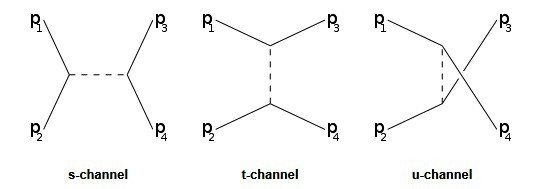
\includegraphics[width=1\textwidth]{figures/stu.jpg}
    \caption[Particle interactions through $s$, $t$, and $u$ channels]{Respective $s$, $t$ and $u$ channels for proton interactions.}
    \label{tf33}
\end{figure}
\FloatBarrier
Another two variables which are very important in particle physics are rapidity and pseudorapidity. Rapidity is defined as
\begin{equation}
\centering
y=\frac{1}{2}ln\left(\frac{E + p_zc}{E - p_zc}\right)
\label{t10}
\end{equation}
where $E$ stands for energy of a particle and $p_z$ momentum along the $z$ axis. Rapidity is also regarded as "velocity in the longitudinal direction" in high energy physics because  rapidity reduces to velocity in the non-relativistic limit. Rapidity is not a Lorentz invariant but it does hold a large role in detector physics. Pseudorapidity, $\eta$, is defined as the following,
\begin{equation}
\centering
\eta = -ln\left(tan~\frac{\theta}{2}\right)
\label{t11}
\end{equation}
where $\theta$ is the angle between the direction of an outcome particle and the $z$ axis. Pseudorapidity does have an advantage over rapidity- it is represented only by 1 independent variable, while rapidity needs energy and momentum to be defined. For high energy collisions, when it is possible to neglect the mass of particles, rapidity, and pseudorapidity coincide. Pseudorapidity ranges from 0 to infinity. Small angles of $\theta$ characterize diffraction therefore, the values for pseudorapidity of scattered protons are very big. 
\newline
The last and most important quantity of particle physics is cross-section $\frac{\mathrm{d}\sigma}{\mathrm{d} \Omega}$. The differential cross section is the probability per unit solid angle that an incident particle is scattered into the solid angle $\mathrm{d}\Omega$ \cite{Krane}. For easier computation, some assumptions have to be made. The densities of incident particles and target particles are considered to be small enough that they interact only once with each other, and that the energy that binds the target particles to their place is negligible compared to the energy of the incident particles. It is recognized as $\sigma$, but much more often, it is used in differential form as $\frac{\mathrm{d} \sigma}{\mathrm{d} x}$, where $x$ is a kinematic variable.
\begin{equation}
\centering
R_{int} = L \frac{\mathrm{d} \sigma}{\mathrm{d} \Omega}(\theta, \varphi)
\label{t25}
\end{equation}
\autoref{t25}, is a typical equation for the interaction rate $R_{int}$ of particles colliding in a collider. $L$ is luminosity, and it represents the properties of the collider, but not the particles themselves. Luminosity can be quite difficult to measure accurately. Therefore, it is one of the biggest sources of errors in collider physics. $\frac{\mathrm{d} \sigma}{\mathrm{d} \Omega}(\theta, \varphi)$ is the differential cross-section depending on the scattering angle. 

\FloatBarrier
\begin{figure}[ht]
    \centering
    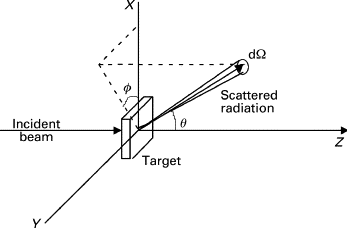
\includegraphics{figures/cs.png}
    \caption[Diagram of a scattering of a particle]{Diagram of a scattering of a particle into the solid angle $\mathrm{d}\Omega$. Taken from Ref.~\cite{cs}.}
    \label{tf32}
\end{figure}

\section{Particle diffraction}
The name diffraction comes from the analogy with optical diffraction, which is a phenomenon that occurs when a plane electromagnetic wave moves through a hole in a screen. The wave behind the screen lands on a detector plane, where intensity is measured. The Huygens-Fresnel principle states that every point in the hole in 
the screen becomes a unique source of a spherical electromagnetic wave, and what one can see on the detector is the interference of these sources of light. The analogy between particle and optic diffraction is the collision or interaction of 2 objects with similar wavelengths\footnote{Thanks to de Broglie hypothesis, it is possible to look at quantum particles as waves.}. The wave description is used because diffractive interaction is an ultra peripheral process. Particle diffraction has several definitions. The first definition was formulated by Good and Walker~\cite{GoodWalker} in 1960:
\newline
\newline
\textit{A reaction in which no quantum numbers are exchanged between the colliding particles is, at high energies, a diffractive reaction.}
\newline
\newline
In other words, diffraction has to satisfy 2 conditions- no quantum numbers\footnote{Quantum numbers understood as electrical charge, orbital angular momentum, spin, parity...} can be exchanged, and the collision must be at high energies. It is quite a straight-forward definition yet not entirely practical.  That is why an equivalent and more practical definition was formulated in lectures at Stanford University by Bjorken~\cite{Bjorken} in 1994.
\newline
\newline
\textit{A diffractive process occurs if and only if there is a large rapidity gap in the produced particle phase space, which is not exponentially suppressed.}
\newline
\newline
It translates to a simple condition that between forward and backward scattered protons and the hadron pair have to exist clear gaps in rapidity. Large rapidity gap is not exclusive for diffractive events, but all other events are exponentially suppressed. The number of diffractive events is somewhat constant with different energy of collision. In the next part, I will reproduce the calculation of the Large rapidity gap, as it is described in Ref.~\cite{Barone}. Even though it is almost an identical recreation, it is crucial for this thesis and the topic of diffraction. The computation and the following physical results are noted using natural units\footnote{Computation with natural units assumes the universal constants such as $\hbar$ or $c$ to be equal to 1.}.
\newline
Let us consider a high energy semi-inclusive collision where $p_1$, $p_2$ are 4-momentum vectors of colliding particles and $p_3$ represents the 4-momentum of an unaltered particle after the collision. For simplicity, the masses of the 3 particles are all the same and equal to $m$. 
\begin{equation}
\centering
p_1 = (E_1,0,0,p_z)
\label{t13}
\end{equation}
\begin{equation}
\centering
p_2 = (E_2,0,0,-p_z)
\label{t14}
\end{equation}
\begin{equation}
\centering
p_3 = (E_3,p_x^{'}, p^{'}_y ,p_z^{'})
\label{t15}
\end{equation}
As mentioned before, because of cylindrical symmetry, transverse momentum is used $p^{'}_T = \sqrt{p_x^{'2} + p_y^{'2}}$. Because the transverse momentum before the collision is 0, this condition has to be the same also after the collision, and therefore the sum $p_T$ of all product particles must equal to 0. In high energy approximation, the following equations are achieved,
\begin{equation}
\centering
\left|p^{'}\right| \approx \frac{s - M^2}{2\sqrt{s}}
\label{t17}
\end{equation}
\begin{equation}
\centering
\left|E_3\right| \approx \frac{s - M^2}{2\sqrt{s}}
\label{t18}
\end{equation}
where $M$ corresponds to the mass of a system of particles $X$, which is not measured. $s$ is above mentioned Mandelstam variable. Because a diffractive process is considered, transverse momentum will be significantly smaller than momentum along $z$ axis, therefore $\left|\vec{p}_z^{~'} \right| \simeq \left| \vec{p}^{~'} \right|$. It is possible to establish a variable called transverse mass,
\begin{equation}
\centering
m^{'}_{T} = \sqrt{m^2 + p^{'2}_{T}}
\label{t24}
\end{equation}
which is invariant under Lorentz transformation. Once again, if the mass of particles is approximated to be insignificant, the rapidity takes the form of the following equation.
\begin{equation}
\centering
y \approx ln \frac{2p_z}{m_{T}}
\label{t16}
\end{equation}
If all the aforementioned relations are combined, the rapidity of the 3. particle can be obtained.
\begin{equation}
\centering
y_3 \approx ln \frac{\sqrt{s}}{m^{'}_{T}}
\label{t19}
\end{equation}
The maximum value for this quantity corresponds to transverse momentum $p_{T}=0$.
\begin{equation}
\centering
y_{3max} \approx ln \frac{\sqrt{s}}{m}
\label{t20}
\end{equation}
The average and maximum value of the rapidity of system $X$ can be easily obtained.
\begin{equation}
\centering
\left<y_X\right> \approx -ln \frac{\sqrt{s}}{M}
\label{t21}
\end{equation}
\begin{equation}
\centering
\left|y_{X}\right|_{max} \approx ln \frac{\sqrt{s}}{m}
\label{t22}
\end{equation}
From these relations the rapidity gap between particle 3 and edge of the distribution of $X$ system takes the form of \autoref{t23}.
\begin{equation}
\centering
\Delta y \approx ln \frac{s}{M^2}
\label{t23}
\end{equation}
Because the mass of particles is neglected, pseudorapidity takes the same exact form.
\FloatBarrier
\begin{figure}[ht]
\centering
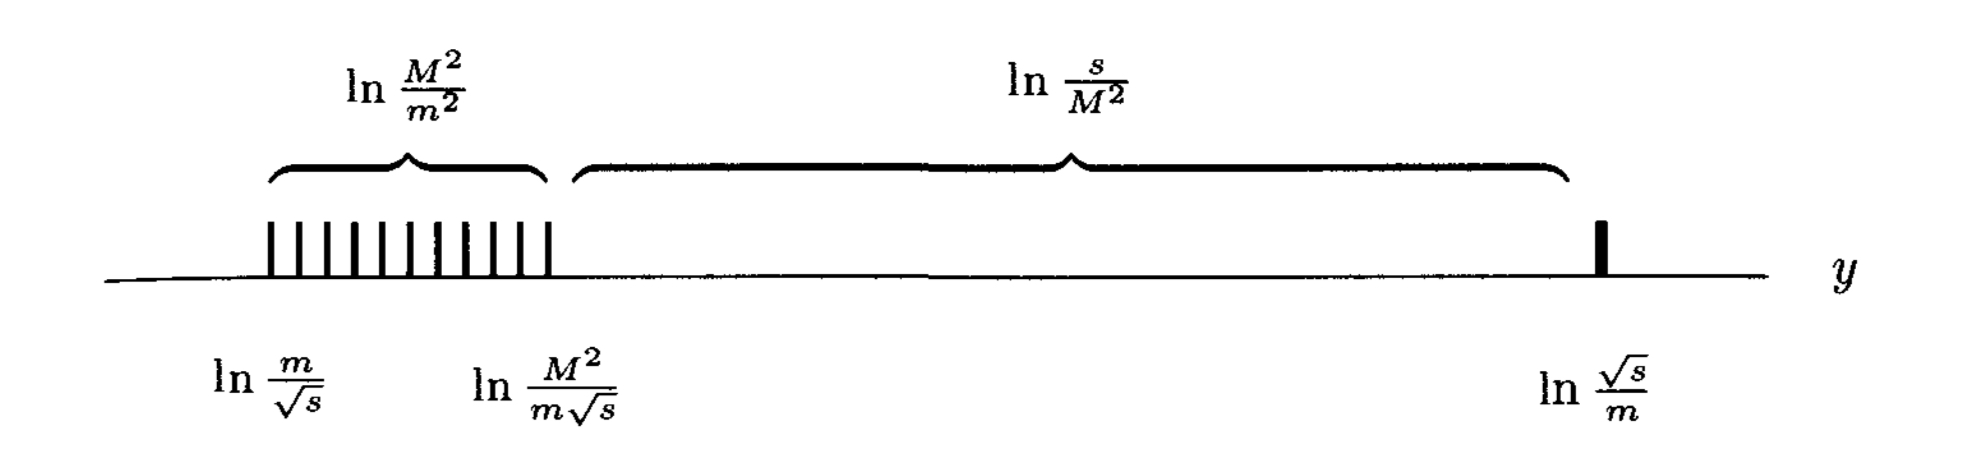
\includegraphics[width=1\textwidth]{figures/rapiditygap.jpg}
\label{tf1}
\caption[Large rapidity gap]{Graphical representation of rapidity gap between the unaltered particle 3, which is on the right side, and the system of particles $X$, which is on the left side. Taken from Ref.~\cite{Barone}.}
\end{figure}
\FloatBarrier


\section{Introduction to Regge theory}
One of the main ideas of Quantum mechanics is the fact that some variables are discrete. In other words, energy or angular momentum are not a continuous spectrum but can occupy only certain permitted values. These values depend later on the type of system and it's properties. Regge~\cite{Regge}, with his theory, went beyond that. He discusses the idea of extending the angular momentum range not only to all real values but also to complex values. Regge explained his idea on the scattering of a quantum particle on potential. He introduced complex angular momentum which depends on the energy of the collision. Such an approach leads to the distribution of energy which is known as Breit-Wigner energy distribution\footnote{Breit-Wigner distribution is a consequence of Heisenberg uncertainty principle. Incorporating a complex variable in quantified values results in the distribution of the quantity, and therefore, the uncertainty of the exact value. More in Ref.~\cite{Breit1936}}. Even though the theory is called after Tullio Regge, great contributions came from Geoffrey Chew and Steven Frautschi, who established a connection between Regge's extension of angular momenta and actual particles. Regge began the thought process by proposing that mesons and baryons are only bound states. Later Chew and Frautschi advanced the idea by stating that none of the bound states were elementary particles. They also followed up on Regge's trajectories idea by dividing known particles into several groups or families with similar quantum numbers which were based on their dependence of angular momentum on their squared masses. These families are represented in the so-called Chew Frautschi plot~\cite{ChewFrautschi} and can be seen in \autoref{tf4}.  
\newline
The full understanding of Regge theory is far beyond the scope of this thesis, but to introduce \Pom omeron physics it is necessary to understand what does reggeon\footnote{Reggeons are to be understood as something in Regge theory, that is exchanged between 2 particles that collide.} exchange mean. For the purpose of this thesis, high energy collisions with relatively low energy transfer will be considered an the spin of the scattered particle will be neglected. The partial wave expansion of the scattering amplitude $A(s,t)$ can be written as,
\begin{equation}
    \centering
    A(s,t)=16\pi \sum_{l=0}^{\infty}(2l + 1)A_l(s)P_l(cos~\theta_s)
    \label{t27}
\end{equation}
where $P_l(cos~\theta_s)$ is the Legendre polynomial of the appropriate wave amplitude. For fixed energy of collision, $s$, it is possible to reduce the dependence from energy transfer $t$ to only the scattering angle $\theta_s$. Consequently, it is possible to rewrite the dependence $A(s,t) \rightarrow A(s,t(s, cos~\theta_s))$. If equal mass of both incident particles is considered the following equation holds significance.
\begin{equation}
    \centering
    cos~\theta_s = 1 + \frac{2s}{t - 4m^2}
    \label{t28}
\end{equation}
In the limit of $s \rightarrow \infty$, the right-hand side grows quickly and Legendre polynomials are proportional to $s^l$. The partial wave amplitude then reduces to,
\begin{equation}
    \centering
    A_l(s,t) \sim f(t) s^{I}
    \label{t29}
\end{equation}
where $I$ is the spin of the exchanged particle for the certain partial amplitude. Optical theorem states $\sigma_{tot} \sim s^{I - 1}$, where $\sigma_{tot}$ is the total cross section. If all resonance exchanges are summed together and Regge's mathematical representation is used, it is possible to rewrite the partial wave amplitudes to be the following.
\begin{equation}
    \centering
    A(l,t) = A_l(t), {\color{white} \longrightarrow} l = 0, 1, 2...
    \label{t30}
\end{equation}
\begin{equation}
    \centering
    l=\alpha(t)
    \label{t31}
\end{equation}
Complex functions $\alpha(t)$ create poles in the complex $l$ plane. The sum of all the partial wave amplitudes gives the resulting scattering amplitude along with the total cross section shape~\cite{PomeronPhysics}. For \DPE~between 2 protons, the shape is shown in \autoref{tf5}. The total cross section is rising, which was first stated by Gribov and is well described in Ref.~\cite{gribov2003}.
\FloatBarrier
\begin{figure}[ht]
    \centering
    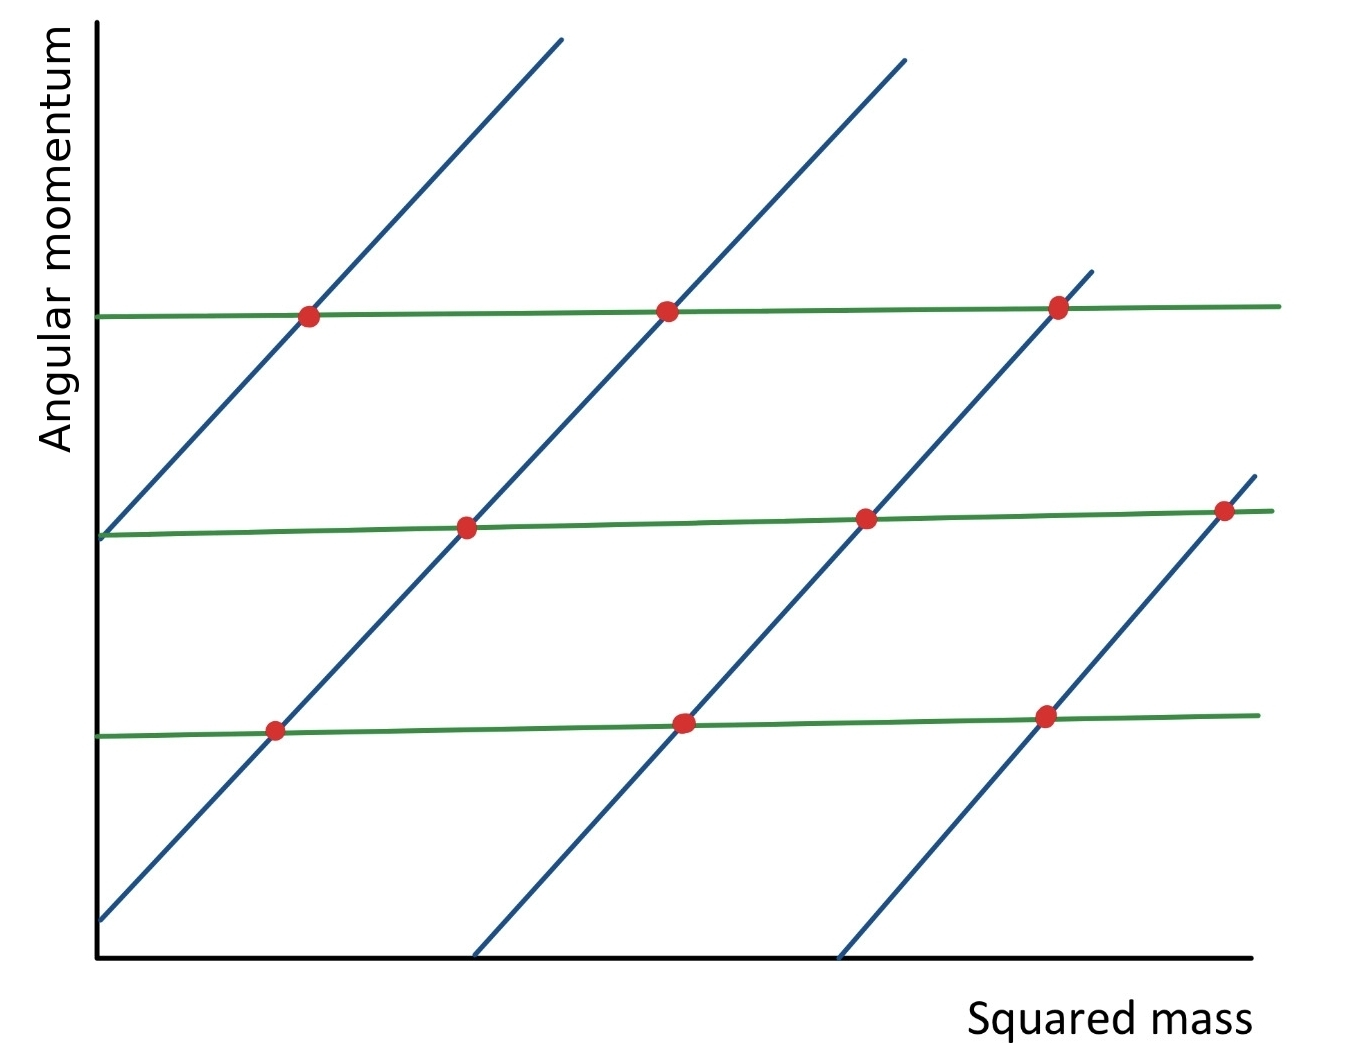
\includegraphics[width=0.7\textwidth]{figures/CFplot.jpg}
    \caption[Chew-Frautschi plot]{The Chew Frautschi plot of angular momentum dependence on squared mass. Blue lines represent Regge trajectories and red intercepts represent the bound states of particles. }
    \label{tf4}
\end{figure}
\FloatBarrier
\section{Pomeron process}
\label{Pomeronprocess}
\Pom omeron is a Regge trajectory, typical for diffractive events. It takes the name after the soviet physicist, Pomeranchuk, who has contributed to particle physics in many ways including the Pomeranchuk theorem which states that under some conditions the total cross sections of a particle and a corresponding antiparticle scattering on the same target becomes asymptotically same~\cite{PomeronPhysics}.
\newline
In this thesis, proton proton diffractive events at the center of mass energy $\sqrt{s} = 510$ GeV are studied, which are very well described with the so-called Double \Pom omeron exchange (\DPE). Another process, which creates a different system of particles, is called photoproduction and is described with the exchange of one \Pom omeron and one virtual photon. As mentioned before, the measured process is \autoref{t26}. The detector then detects hadron pairs which are mostly $\pi^+ \pi^-$, sometimes $K^+ K^-$ or $p \overline{p}$. Some processes may include a combination of these particles. On the other hand, particle $J/\psi$ decays to an electron-positron pair.
\FloatBarrier
\begin{figure}[ht]
    \centering
    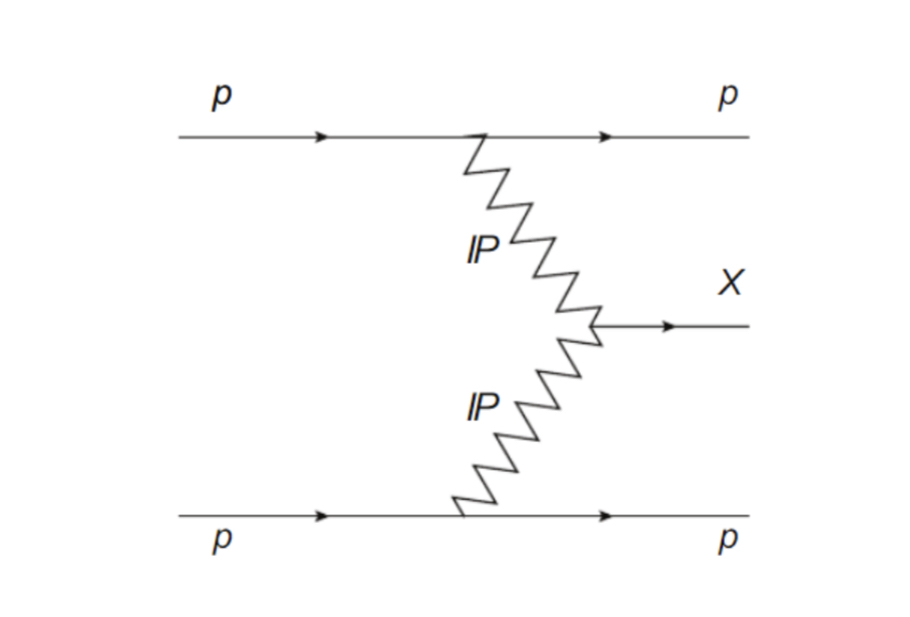
\includegraphics[width=0.7\textwidth]{figures/pomeronprocess.jpg}
    \caption[Double \Pom omeron exchange]{Double \Pom omeron  process between 2 protons with the result of the creation of another particle. The crisscross line represents the exchange of a \Pom omeron. Feynman diagram taken from Ref.~\cite{Guryn2016}.}
    \label{tf3}
\end{figure}
\FloatBarrier
Even though Regge theory has been developed for quite some time, the physical meaning of \Pom omeron is still quite unclear. The quantum numbers of \Pom omeron are the same as the quantum numbers of vacuum, isospin 0, and even charge parity, which does not correspond to any known particle. From experimental results, the \Pom omeron trajectory is expected to be a linear dependence on momentum transfer $t$~\cite{Albrow_2010}.
\begin{equation}
    \centering
    \alpha_{\mathbb{P}}(t) \sim \alpha_{\mathbb{P}}(0) + \alpha_{\mathbb{P}}^{'} = 1.08 + (0.25~\mathrm{GeV}^{-2})t
    \label{t32}
\end{equation}
Quantum chromodynamics describes the process (in the first approximation) as the exchange of 2 gluons. QCD predicts the existence of so-called glueballs, which are objects made up by 2 gluons or more. Glueballs have not yet been observed, but the studying the topic of \DPE~ will bring physicists closer to it's understanding and possibly even future confirmation, which would strongly support Quantum Chromodynamics. 

\section{Recent results}
\label{recent}
First of all, it is necessary to mention, that the measurement of $K^{0}_s$ (upon which will be the focus of this thesis) in diffractive proton-proton collisions at energies $\sqrt{s}=510$ GeV has never been done before. There have been similar measurements at experiment STAR and at different colliders and detectors. Even though there have been attempts to measure proton-proton collisions and \DPE~in the 1960s and 1970s, the first collider that was able to collide hadrons was the collider Intersecting Storage Rings (ISR). Previous experiments did not acquire enough energy to create 2 Large rapidity gaps~\cite{Albrow_2017}. Intersecting Storage Rings brought the first data of \DPE.
\FloatBarrier
\begin{figure}[ht]
    \centering
    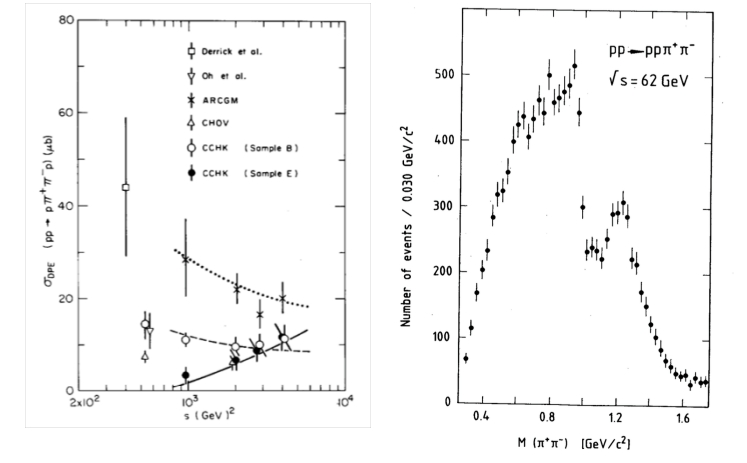
\includegraphics[width=0.9\textwidth]{figures/ISR.jpg}
    \caption[Cross section of pp collisions from ISR]{Left: Graph shows the dependence of cross section of \DPE~on ISR energies of collisions with respective fits of Regge trajectories. Right: Graph shows the central exclusive production of $\pi^{+}\pi^{-}$ production rate on invariant mass. Taken from Ref.~\cite{Albrow_2017}.}
    \label{tf6}
\end{figure}
\FloatBarrier
\FloatBarrier
\begin{figure}[ht]
    \centering
    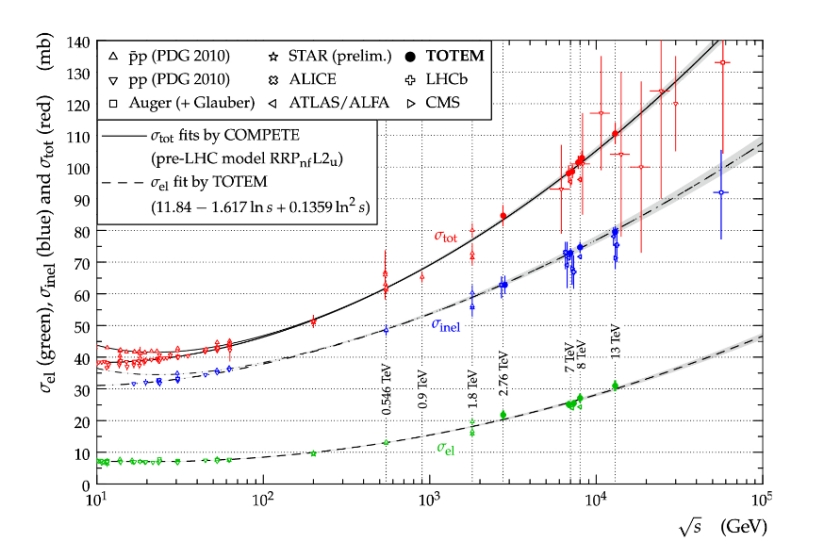
\includegraphics[width=0.9\textwidth]{figures/cspp.jpg}
    \caption[Cross section of pp and p$\overline{p}$ from different experiments]{Graph of cross section dependence on energy of proton-proton or proton-antiproton collisions measured at experiments STAR, ALICE, ATLAS, TOTEM, LHCb, CMS and AUGER. Green represents data from elastic collisions, blue is inelastic and red is total cross section. Taken from Ref.~\cite{zyla}.}
    \label{tf5}
\end{figure}
\FloatBarrier
The measurements of proton-proton collisions have gone a long way since the times of ISR. Such processes have been measured at all the significant experiments at different energies \autoref{tf5}. Most of the measurements are semi-exclusive: the outgoing protons are not tagged or measured. The only experiment, that is able to perform analysis on exclusive processes is the experiment STAR at RHIC, and it is thanks to subdetectors called Roman Pots. The latest article from the STAR collaboration on \DPE~is Ref.~\cite{Rafal20}, \textit{Measurement of the central exclusive production of charged particle pairs in proton-proton collisions at $\sqrt{s} = 200$ GeV with the STAR detector at RHIC}. The author discusses mainly the continuous creation of hadron pairs $\pi^+ \pi^-$, $K^+ K^-$, and $p\overline{p}$ and analyzes the cross section dependence on different variables such as the invariant mass of the created pair. 
\FloatBarrier
\begin{figure}[ht]
    \centering
    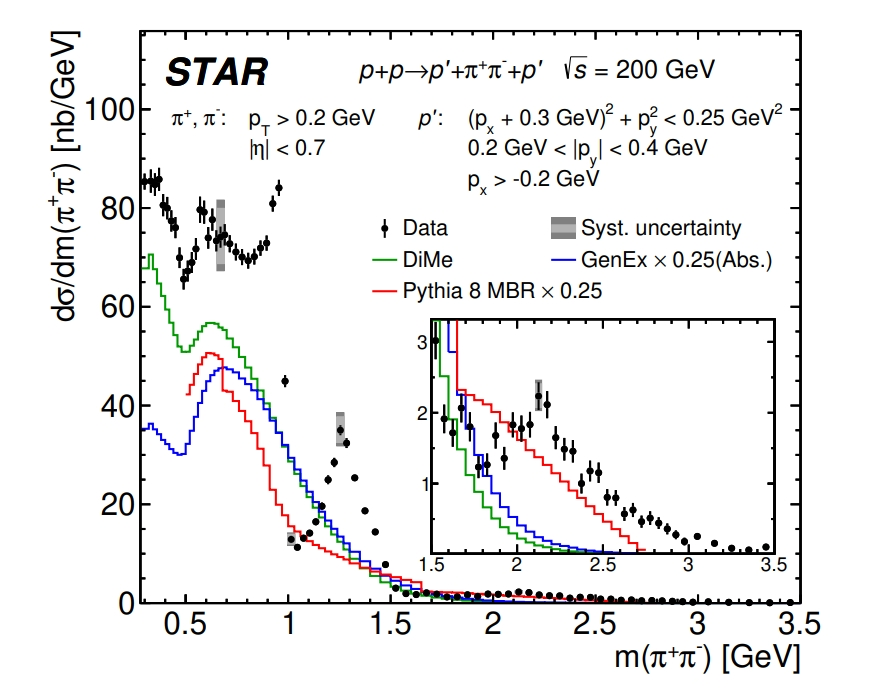
\includegraphics[width=1\textwidth]{figures/rafalpi.jpg}
    \caption[Cross section dependence on invariant mass for $\pi^+ \pi^-$ pairs at STAR]{Graph of cross section dependence on invariant mass of $\pi^+ \pi^-$ pair with 3 Monte Carlo simulations based on different phenomenological models. Taken from Ref.~\cite{Rafal20}.}
    \label{tf7}
\end{figure}
\FloatBarrier
For pion pair invariant mass, resonances $f_0$(980) and $f_2$(1270) were observed and expected to be the products of \Pom omeron- \Pom omeron fusion\footnote{\Pom omeron- \Pom omeron fusion is the continuous production equivalent to \DPE~in resonant production.}. Resonance $f_0$(980) can be seen in the graph at 0.98 GeV as a slight increase after which is a very steep drop. Resonance $f_2$(1270) follows after and can be seen at 1.27 GeV. Similar structures are seen in an independent study \cite{Truhlar}. 
\newline
According to Minkowski and Ochs, a very wide light scalar glueball might be located between 0.4 and 1.7 GeV. They call it the Red Dragon~\cite{Truhlar}. The same peaks can be seen in \autoref{tf6}. The author also noticed a resonance at around $\sim 2.2$ GeV which was not described by the Monte Carlo models. The simulations only predict continuous production and not the resonances.
\newline
Resonances $f_2$(1270) and $f^{'}_2$(1520) for kaons were measured, corresponding to previous measurements at lower energies. These resonances are also expected to be involving the \Pom omeron- \Pom omeron fusion. The statistics for $p\overline{p}$ were quite insignificant with large uncertainties, but there seems to be no significant resonances as in $\pi^+ \pi^-$ distribution.
\FloatBarrier
\begin{figure}[ht]
    \centering
    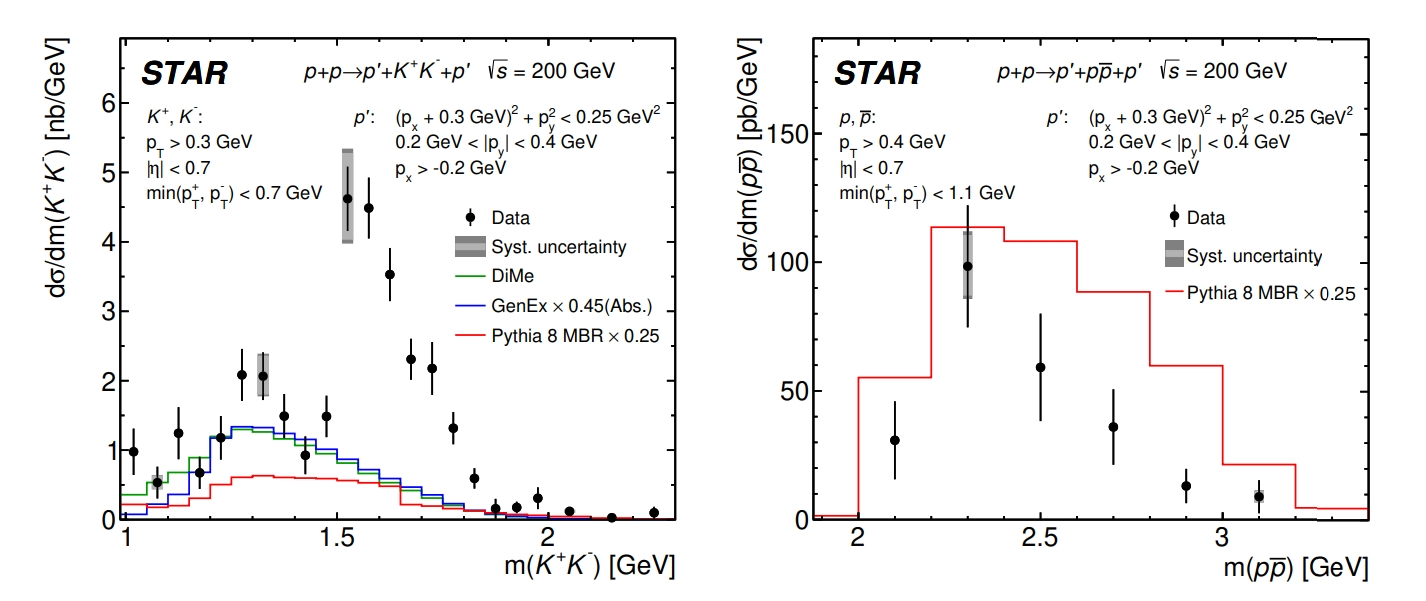
\includegraphics[width=1\textwidth]{figures/raphalkp.jpg}
    \caption[Graphs of cross section dependence on invariant mass of $K^+ K^-$ and $p \overline{p}$ pairs at STAR]{Graphs of cross sections dependence on invariant mass of $K^+K^-$ on the left and $p \overline{p}$ pairs on the right. Taken from Ref.~\cite{Rafal20}.}
    \label{tf8}
\end{figure}
\FloatBarrier
\begin{figure}[ht]
    \centering
    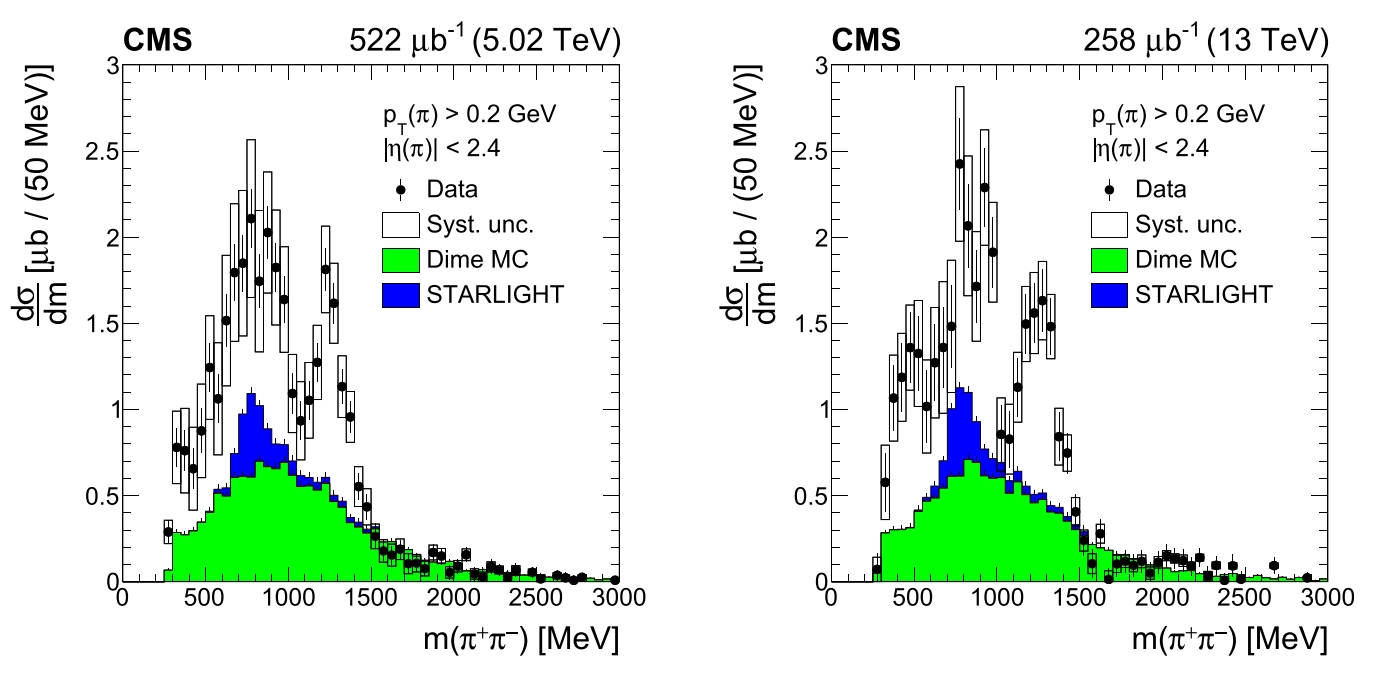
\includegraphics[width=1\textwidth]{figures/CMS.jpg}
    \caption[Cross section dependence on invariant mass of $\pi^+ \pi^-$ pairs at CMS]{Graphs of cross section dependence on invariant mass of created pion pair at $\sqrt{s}=5.02$ and $13$ TeV at CMS. Taken from Ref.~\cite{Sirunyan_2020}.}
    \label{tf8}
\end{figure}
\FloatBarrier
Another interesting measurement~\cite{Sirunyan_2020} was done at the CMS experiment at the Large hadron collider in CERN at energies $\sqrt{s} = 5.02$ and $13$ TeV. 4 resonant channels were extracted. The resonances are $f_0$(500), $\rho^0$(770), $f_0$(980) and $f_2$(1270). The latter 2 correspond previously mentioned resonances. Results for calculated cross sections of resonances are listed in table below.
\FloatBarrier
\begin{table}[ht]
    \centering
    \begin{tabular}{c|c|c}
        \
               & $\sqrt{s}$=5.02 TeV & $\sqrt{s}$=13 TeV \\ \hline
    $f_0$(500) & 2.8 $\pm$ 1.4(stat) $\pm$ 2.2(sys) & 2.2 $\pm$ 0.8(stat) $\pm$ 1.3(sys) \\
    $\rho^0$(770) & 4.7 $\pm$ 0.9(stat) $\pm$ 1.3(sys) & 4.3 $\pm$ 1.3(stat) $\pm$ 1.5(sys) \\
    $f_0$(980) & 0.5 $\pm$ 0.1(stat) $\pm$ 0.1(sys) & 1.1 $\pm$ 0.4(stat) $\pm$ 0.3(sys) \\
    $f_2$(1270) & 3.6 $\pm$ 0.6(stat) $\pm$ 0.7(sys) & 4.2 $\pm$ 0.9(stat) $\pm$ 0.8(sys) 
    \end{tabular}
    \caption[Results of measured cross sections for 4 resonant channels at CMS]{Table of total cross sections of observed resonances in pion production based on the energy of collisions. Data taken from experiment CMS~\cite{Sirunyan_2020}.}
    \label{tt1}
\end{table}
\FloatBarrier
 % Theoretical introduction
\newpage
\chapter{The STAR detector and RHIC collider}
\label{detector}
The relativistic heavy ion collider (RHIC) is located at Brookhaven National Laboratory (BNL) on Long Island, in the state of New York. The facilities were rebuilt after the end of World War II from a U.S. Army camp into the scientific and technological laboratory it is now. It is one of several national laboratories under the United States Department of Energy administration. 
\newline
Brookhaven National Laboratory has a long history with particle physics. The first accelerator at BNL was the Cosmotron which operated between the years of 1952 and 1966. Brookhaven was and still is home of many accelerators such as the Alternating Gradient Synchrotron, National Synchrotron Light Source I or the newest National Synchrotron Light Source II. The above mentioned RHIC began operating in 2000 and is discussed thoroughly in \autoref{RHIC}. Until the Large Hadron Collider began operation in 2010, RHIC was the highest energy collider in the world. Relativistic Heavy Ion Collider will be running until 2025, when it will be replaced by the Electron Ion Collider. The future of particle physics at BNL is discussed in \autoref{EIC}.

\section{RHIC}
\label{RHIC}
The Relativistic Heavy Ion Collider has been operating since 2000, but the work and planning has begun long before. The idea was proposed 16 years earlier~\cite{RHIChis}. RHIC is capable of accelerating protons for proton-proton collisions up to energies of 510 GeV. In nuclei nuclei collisions, the maximum energy is 200 GeV per nucleon. Generally, gold nuclei are used for collisions, but nuclei of elements such as copper, deuterium, Helium or many others have been used. The circumference of the collider is 3834 m \cite{Dehmelt}.

The largest detector at RHIC was the PHENIX detector. The name stands for Pioneering High Energy Nuclear Interaction eXperiment. The development began in 1991 and the goal of the experiment was to measure the Quark-Gluon Plasma\footnote{The Quark-Gluon Plasma is a state of matter created right after the collision of 2 nuclei, when the bonds between elementary particles quarks and gluons are overcome and for a brief moment, they are capable of moving freely. Some theories state that QGP was the only state of matter for a brief moment right after the big bang.} (QGP) and extreme states of matter. Another goal of the experiment was to measure where does the proton gets spin from \cite{PHENIX}.  PHENIX, at \autoref{df1}, is located at 8 o'clock of the RHIC circle. Data taking was done between the years of 2000 and 2016. After a couple of years of inactivity, a new project was born- sPHENIX. This updated version of PHENIX will begin operation in the year of 2023 and will continue until the end of RHIC in 2025. 

\FloatBarrier
\begin{figure}[ht]
    \centering
    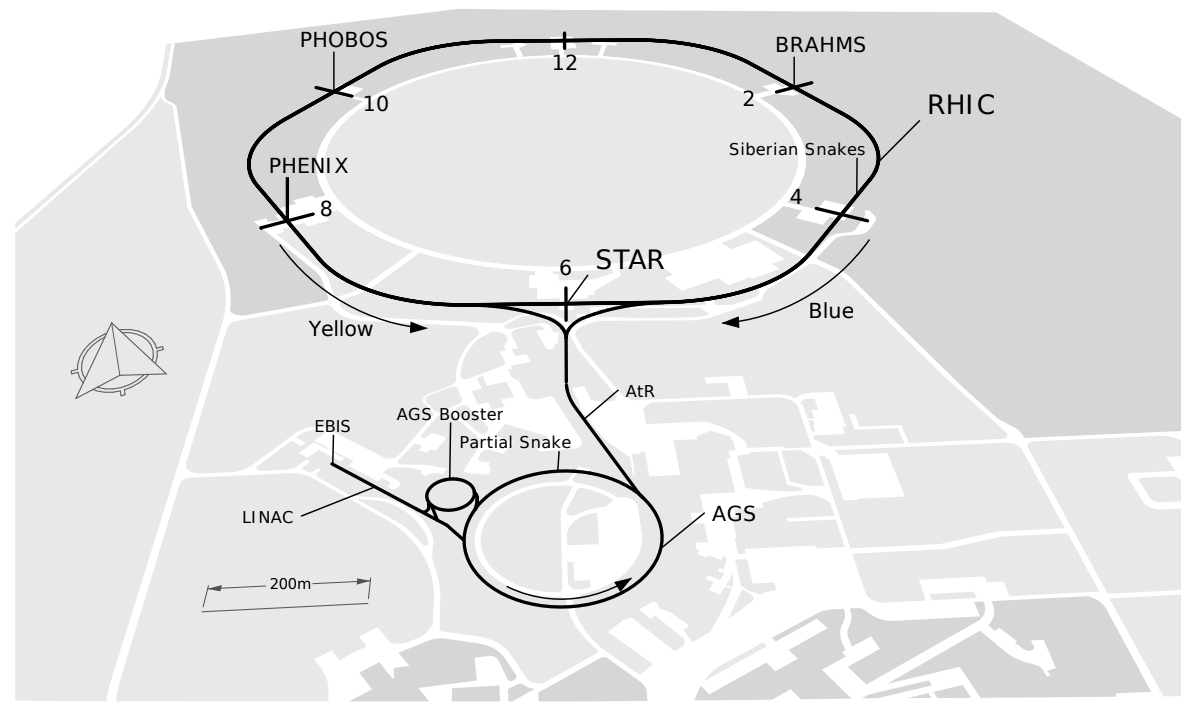
\includegraphics[width=0.9\textwidth]{figures/rhic.jpg}
    \caption[The Relativistic Heavy Ion Collider]{A sketch of the Relativistic Heavy Ion Collider with it's accelerators EBIS, Linac, AGS Booster, AGS and detectors PHENIX, PHOBOS, BRAHMS and STAR. Taken from \cite{STARgraphicsrep}. }
    \label{df1}
\end{figure}
\FloatBarrier

Next in line were PHOBOS and BRAHMS experiments. Their operating times were shorter compared to the other 2 experiments. Data taking began in 2000 and ended in 2005 at PHOBOS and 2006 at BRAHMS. PHOBOS was designed to study a large number of Au-Au collisions and create a big picture description of all sorts of events that happen during a collision. It was capable of measuring the total number of produced particles created in 1 event thanks to many silicon detectors surrounding the point of collision \cite{PHOBOS}. Even though BRAHMS was installed for the first beams in 2000, fully operational was only in 2001. The goal of the detector was to accurately identify particles with the largest possible rapidity range. The results from experiments done at BRAHMS were meant to be complimentary to measurements done at the other 3 experiments at RHIC \cite{BRAHMSadamczyk}. 
\newline
The last detector at the Relativistic Heavy Ion Collider is the STAR detector. It is located near the place at the collider, where accelerated particles enter the collider. STAR detector is the longest operating detector at RHIC. It has been operating since the beginning in 2000 and is planned to work until 2025. The entire detector consists of many subdetectors and systems, which are closely described in \autoref{STAR}. 

Particles that collide in RHIC, go through several accelerators where they gain the desired energy for collision. This is called the pre-injectory system. The source for ion beams is the Electron Beam Ion Source. It creates ion beams which are sped up by 2 small linear accelerators, that carry the beams to the Booster Synchrotron~\cite{RHIC}. For proton collisions, protons are accelerated in the Linear accelerator (Linac) which brings them to Booster. The Booster Synchrotron is able to accelerate beams of particles from 200 MeV up to around 1.2 GeV and holds the role of pre-accelerator for the Alternating Gradient Synchrotron (AGS). AGS is capable of accelerating ions from around 37 $\%$ to 99.7 $\%$ speed of light in vacuum. The synchrotron relies highly on focusing the beam of particles which increases efficiency and reduces costs of operation. The focusing is done by alternating the gradient of the magnetic field~\cite{Adams}. Accelerated ions from AGS move through AGS-to-RHIC line. At the end of the beam line is a magnet, which curves the trajectories of ions and particles either to clockwise which is the "blue" beam line, or counter clockwise direction which is the yellow beam line. Once the beams are in RHIC, they get the final acceleration kick up from radio waves, which brings the speed of ions very close to the speed of light and are ready to be collided. Particles that have been collided inside the Relativistic Heavy Ion Collider are protons, deuterons, nuclei of gold, aluminium, hydrogen, copper, zirkonium and ruthenium. 

\section{STAR detector}
\label{STAR}
The name STAR comes from the abbreviation Solenoidal Tracker At RHIC. The detector itself has gone a long way since it has been installed in 2000. Almost all parts of the detector have been upgraded or somehow improved since 2000 and several detectors have been added. This chapter discusses primarily the current STAR detector's condition, but due to lack of reliable sources, some aspects of the detector discussed in this chapter  might not be entirely up to date. 
\newline
Data for this thesis were measured in 2017, a couple years before a quite large upgrade of several detectors. The upgrade was called BES II\cite{BESII}. It focused on expanding the range of acceptance and the increasing the measuring capabilities of the forward region. Subdetectors Time Projection Chamber (TPC), Time Of Flight detector (TOF), Roman Pot system (RP), Beam Beam Counters (BBC) and Zero Degree Calorimeters (ZDC) will be discussed and some of the others will be mentioned.

\FloatBarrier
\begin{figure}[ht]
    \centering
    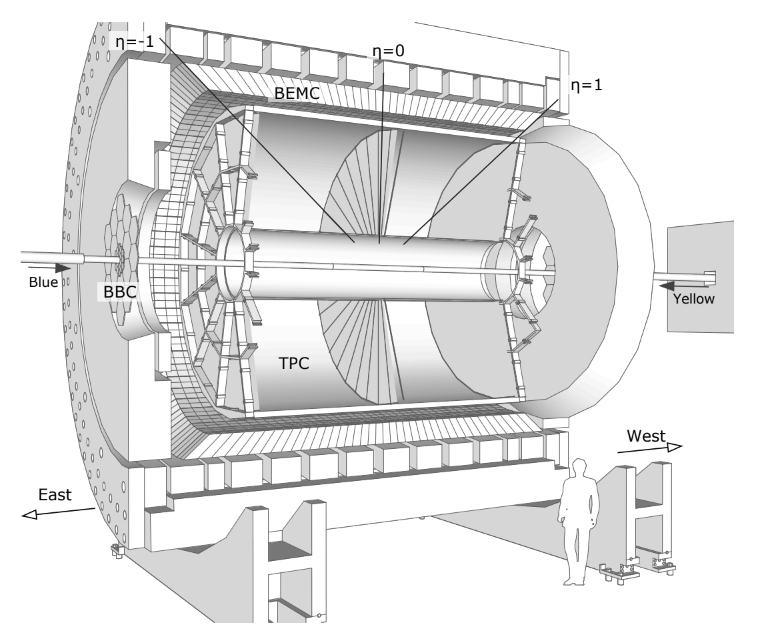
\includegraphics[width=0.65\textwidth]{figures/dete.jpg}
    \caption[Schematic view of the Solenoidal Tracker At Rhic]{A scheme of the STAR detector with names of some subdetectors. Time Projection Chamber in the middle, closest to the interaction point, around it the Barrel Electromagnetic Calorimeter. Beam Beam counters are located in the forward and backward location along the beam pipes Blue and Yellow. Taken from Ref.~\cite{dete}.}
    \label{df4}
\end{figure}
\FloatBarrier


\subsection{Time Projection Chamber}
\label{tpc}
Time Projection Chamber is located at the center of the structure. It is a cylindrical volume that surrounds the interaction point. It is 4 m wide in diameter and 4.2 m long. TPC is a ionization detector, which uses electric and magnetic field for trajectory reconstruction as well as for computing the energy loss of particles. Energy loss is extracted from the measured ionization of gas inside the chamber (90 $\%$ Argon, 10 $\%$ Methane) when electrons drift toward the anode on the sides of the cylinder. The anode is divided into several sectors. The number of sectors that detect signal from electrons then defines how well a track of a particle can be reconstructed and how precise is the energy loss computation. It is regarded in \autoref{analysis} as number of hits in TPC. The velocity of electrons defines the readout time of the detector. Ions drift toward the middle of the detector- central membrane. The drift of charged particles is caused by an electric field which is created by 3 different sources: inner field cage, outer field cage and the aforementioned central membrane\cite{STAR}. Electric field in the chamber is uniform and approximately equal to 135 V/cm \cite{TPC}. Magnetic field's operation value inside TPC is 0.5 T and is created by massive magnetic coils around the detector. The latest upgrade of TPC was BES II. The upgrade involved improving the inner TPC (iTPC) sectors for better understanding of QCD phase diagram. The improvement involved increasing the pseudorapidity by 50 $\%$ up to $|\eta|<1.5$ range, increasing the energy loss and momentum resolutions \cite{TPCupgrade}. This pseudorapidity range of detection is conditioned by a minimum value of particle's transverse momentum (150 MeV). The pad resolution was approximated between 213 and 950 $\mu$m, depending on which part of the pad the particle hits\cite{STAR} (pads are located on the cathodes and are used for reading out signal). TPC was constructed for heavy nuclei collisions which produce quite a lot of particles and fragments, therefore, it has multiplicity rate of more than 3000 tracks per event \cite{TPC}.

\FloatBarrier
\begin{figure}
    \centering
    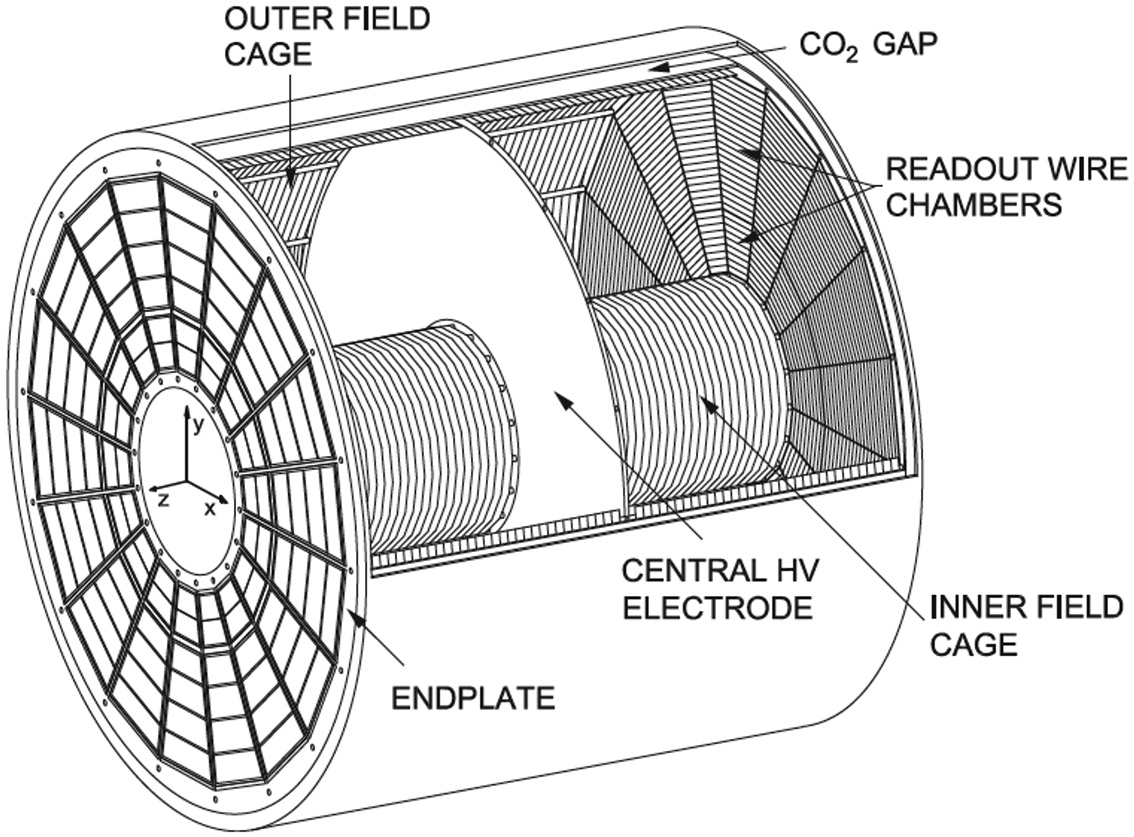
\includegraphics[width=0.8\textwidth]{figures/TPC.png}
    \caption[Schematic view of the Time Projection Chamber]{Scheme of a TPC. Sectors at the endplate detect electrons that are created by ionization of atoms. Taken from Ref.~\cite{sauli_2014}.}
    \label{df11}
\end{figure}
\FloatBarrier

\subsection{Time of Flight detector}
The TOF detector, as can be deduced from the name, measures the time of flight of particles which is then used for particle identification (PID). It is a fast detector with quick readout time which also is used as a trigger. TOF consists of 2 subsystems: the pseudo Vertex Position Detector (pVPD) and the Time of Flight patch (TOFp). pVPDs are located close the the beam line on each side of of the detector and work as a starting point in time for measurement. The TOFp is located around the TPC (exact locations can be seen in \autoref{df5}) and serves as a stopping mechanism for measuring time. pVPDs are plastic scintillators as well as the stop detector, TOFp, which consists of 120 trays. Each tray consists of 32 Multi-gap Resistive Plate Chambers (MRPCs) \cite{MRPC}. The principle of such detectors is that a traversing particle ionizes gas inside and the ejected electrons create electron avalanches (due to electric field) which create signal at the anode \cite{raphalthesis}. The time resolution is 60-100 ps. Part of the BES II upgrade done in 2019, was the expansion of $\eta$ range. The project stemmed from the collaboration of CBM and STAR and meant the installation of CBM modules on east side of the STAR detector. These modules measure range $-1.6<\eta <-1.1$ and their time resolution was measured to be around 83 ps \cite{BESII}. 

\FloatBarrier
\begin{figure}[ht]
    \centering
    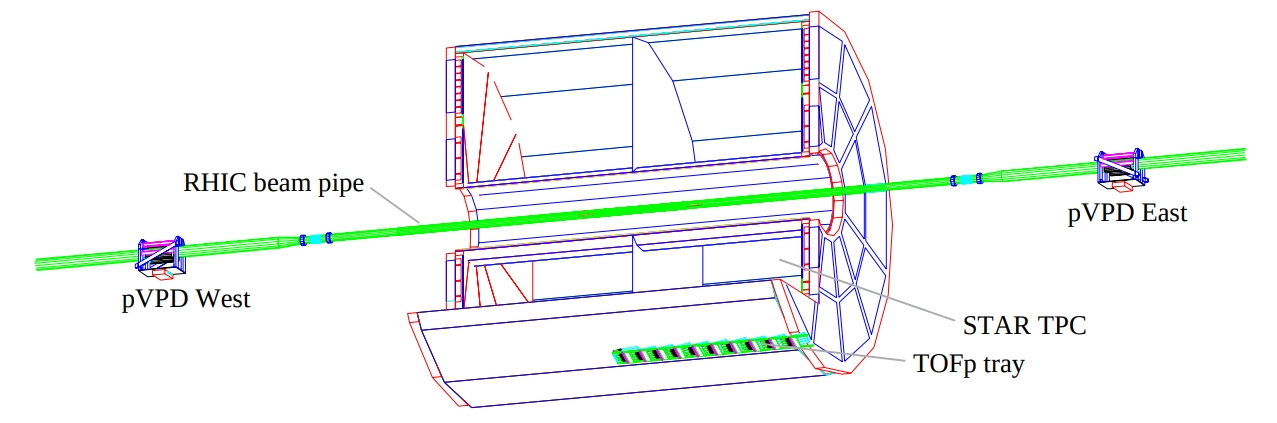
\includegraphics[width=0.9\textwidth]{figures/TOF.jpg}
    \caption[Schematic view of the Time Of Flight detector]{Scheme of Time of Flight detector around the TPC and positions of pseudo Vertex Position detectors which are located 5.6 m away from the center of STAR. Figure taken from Ref.~\cite{TOF}.}
    \label{df5}
\end{figure}
\FloatBarrier

\subsection{Roman Pot system}
\label{RPs}
Roman Pot system holds a crucial role in diffractive physics and detecting forward scattered protons. RPs are designed to measure the $(x,y,z)$ coordinates of protons which are used to reconstruct momenta. Momentum is mostly reconstructed in the transverse direction $(x,y)$. Thanks to the conservation of transverse momentum, such measurement helps to identify exclusive production. Altogether, there are 8 Roman Pots located around the STAR detector and are closely shown and described in \autoref{df6}. Each Roman Pot consists of 4 Silicon Strip Detectors (SSD) and a trigger scintillation counter. The active area of the detector is roughly $79 \times 49$ mm \cite{raphalmsc}. The average efficiency of a Roman Pot is approximately 99.98 $\%$ \cite{STAR}.

\FloatBarrier
\begin{figure}[ht]
    \centering
    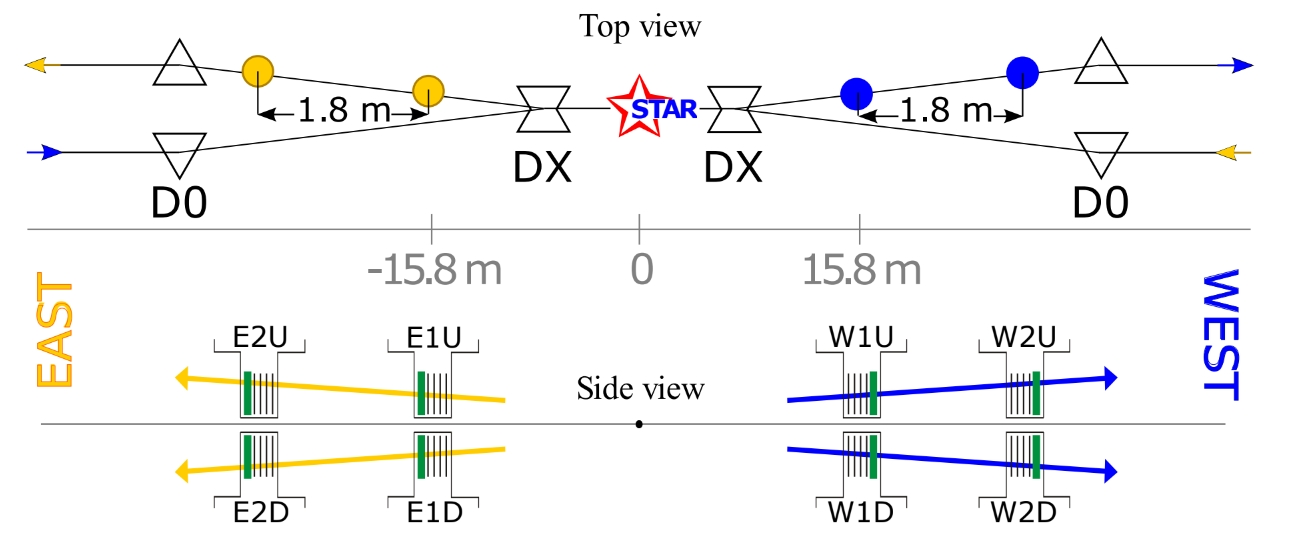
\includegraphics[width=0.85\textwidth]{figures/RP.jpg}
    \caption[Schematic view of the Roman Pot system]{Scheme of layout of the Roman pots. DX and D0 are magnets which curve the trajectories of the charged particles. Each Roman Pot is denoted with 3 different characters based on the position. E and W for east and west, 1 or 2 for position closer and further from the STAR detector, and U or D for up or down based on whether $y>0$ or $y<0$. The positions 1 and 2 are located 15.8 and 17.6 m away from the center of STAR. Taken from Ref.~\cite{raphalthesis}.}
    \label{df6}
\end{figure}
\FloatBarrier

\subsection{Beam Beam Counters}
Beam Beam counters are located on both sides of the cylindrical shape of TPC at around 3.75 m from the interaction point, as can be seen in \autoref{df4}. BBCs are plastic scintillators of hexagonal shape used mostly for providing minimum-bias trigger and for monitoring the collision rate \cite{raphalthesis}. They fall into 2 subcategories: large BBCs (or BBC-L) and small BBCs (or BBC-S). BBC-L cover the region $2.1<|\eta|<3.3$ and BBC-S range of $3.3<|\eta|<5.0$ \cite{STAR}. The time resolution of BBCs is approximately 900 ps \cite{Truhlar}.


\FloatBarrier
\begin{figure}[ht]
    \centering
    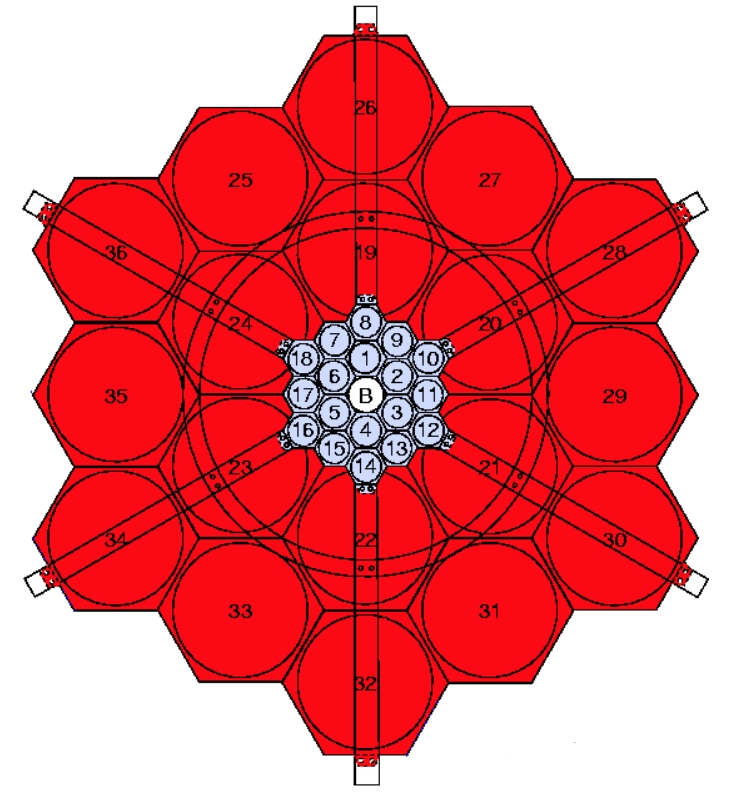
\includegraphics[width=0.6\textwidth]{figures/BBC.jpg}
    \caption[Schematic view of a Beam Beam Chamber]{Schematic view of BBC. Red hexagonal shapes represent the BBC-L, light blue are BBC-S and B in the middle stands for beam line. Taken from Ref.~\cite{STAR}.}
    \label{df7}
\end{figure}
\FloatBarrier

\subsection{Zero Degree Calorimeters}
ZDCs are hadron calorimeters that hold the purpose of detecting neutrons along the beam line. They are located on either side of the detector 18 m away from the interaction point behind the dipole magnets, which are denoted as DX in \autoref{df6}. Because ZDCs are measuring neutral particles, they are positioned at (x,y)=(0,0). The neutron multiplicity plays a significant role in determining the centrality\footnote{Centrality of a collision is determined by the geometry and the degree of overlap in collision and is used mostly in heavy ion collisions. A head-on collision means 0 $\%$ centrality and 2 nuclei missing each other means 100 $\%$ centrality.} of symmetric collisions as well as it provides a way of monitoring luminosity \cite{ZDC}. On each side of the STAR detector is located a ZDC which is constructed out of 3 modules. Each module consists of tungsten plates, fibers and photon multiplier tubes \cite{ZDC}.

\subsection{Other subsystems}
There are a few more parts which do not hold a significant role in analysis for the purpose of this thesis, yet they are worth mentioning. An interesting way of measuring energy of electromagnetic interaction are electromagnetic calorimeters. STAR has 2 of them: Barrel Electromagnetic Calorimeter\cite{BEMC} (BEMC) and Endcap Electromagnetic Calorimeter\cite{EEMC} (EEMC) which cover the full azimuthal angle with ranges of $|\eta|<1$ and $1<|\eta|<2$ respectively. The Muon Telescope Detector (MTD) was installed between the years 2012 and 2014 and is very efficient at identifying muons. This is crucial for identifying heavy quark states through the dilepton decay channel. The MTD covers about 45 $\%$ of the azimuthal angle and measures muons in the range $|\eta|<0.5$ \cite{MTD}. Another detector worth mentioning is Event Plane Detector (EPD) which was installed before run18, in 2018 \cite{BESII}. One on each side covers the range of pseudorapidity $2.1<|\eta|<5.1$. Their objective is to reconstruct event plane and provide information on the geometry of heavy nuclei collisions \cite{EPD}.

\FloatBarrier
\begin{figure}[ht]
    \centering
    \includegraphics[width=0.9\textwidth]{figures/fu.jpg}
    \caption[Schematic view of the STAR detector with highlighted forward upgrade BES II]{Scheme of the STAR detector with highlighted forward upgrade. Light and darker purple near the beam line represent the FTS and FCS. Taken from Ref.~\cite{BNL}.}
    \label{df10}
\end{figure}
\FloatBarrier

Part of the 2019 BES II focus was the forward upgrade. It included Forward Tracking System (FTS) and Forward Calorimeter System (FCS) which both cover the range $2.5<|\eta|<4$. The FTS consists of 4 small-strip Thin Gap Chambers (sTGC) which are capable of measuring transverse particles' momenta in range $0.2<p_T<2$ GeV/c with 20-30 $\%$ momentum resolution \cite{BESII}. The FCS includes a hadron as well as an electromagnetic calorimeter. Though there are a few more subordinate systems of the STAR detector, there is no capacity to discuss them in this thesis.

\section{EIC and the future}
\label{EIC}

The Electron-Ion Collider will be colliding heavy nuclei and protons with electrons which are significantly smaller and lighter. With sufficient energy, it means electrons will not be interacting with the nuclei as a whole, but with sole nucleons, quarks even. This might shine light onto the complex structures of nuclei, but also gluons, sea quarks and valence quarks which make up hadrons. It could uncover the saturation level of quarks that is called color glass condensate \cite{EIC}. Eventually, results from experiments at EIC will bring physicists closer to understanding the strong interaction. Electron-Ion Collider will improve the ability of RHIC to collide polarized protons (up to 70 $\%$), that will furthermore widen the knowledge of proton spin. This will be the first electron-ion collider in the world, therefore, significant results are expected. 
\FloatBarrier
\begin{figure}[ht]
    \centering
    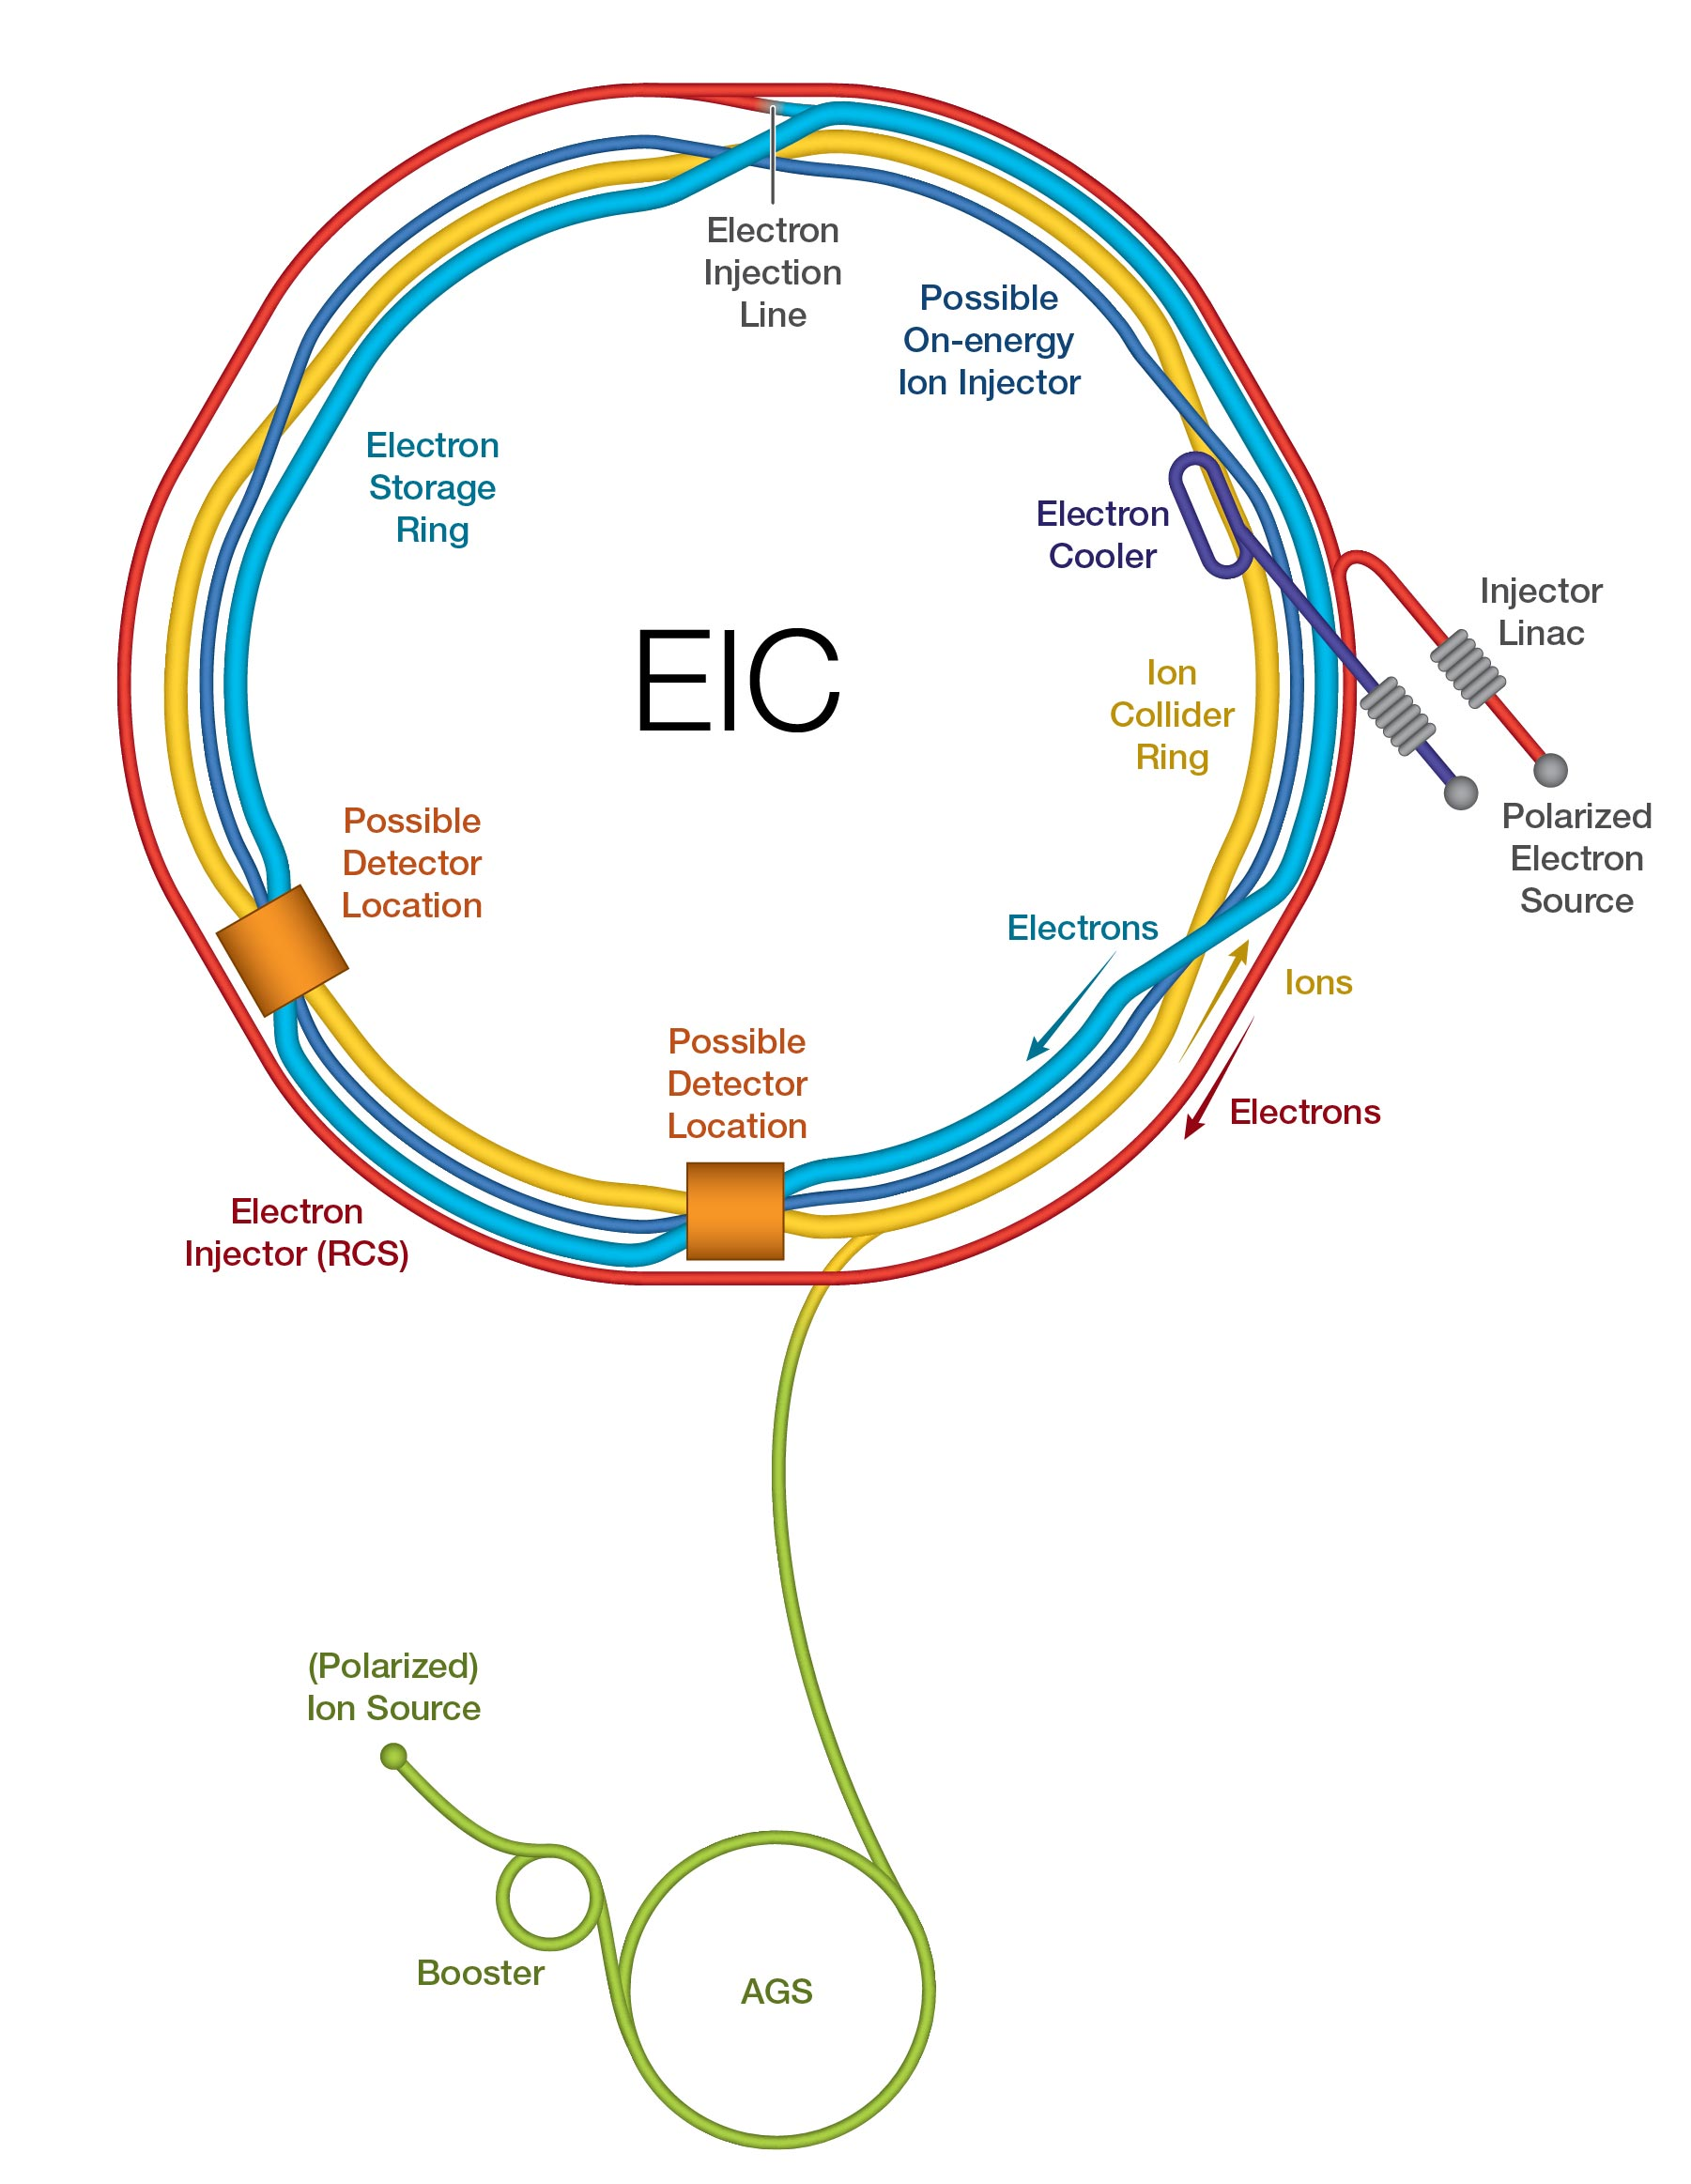
\includegraphics[width=0.7\textwidth]{figures/EIC.jpg}
    \caption[Schematic view of the Electron Ion Collider]{Scheme of the planned structure of Electron-Ion Collider at Brookhaven National Laboratory. Taken from Ref.~\cite{flickr}. }
    \label{df2}
\end{figure}
\FloatBarrier
EIC will be built in the tunnels of RHIC. It will make use of the RHIC's ion accelerators that are already implemented, but will require new electron sources and accelerators as well as a new electron storage ring \cite{EIC}. Even though construction begins after the end of operation of RHIC in 2025, many works have already begun. Simulations of collisions are already being made and detectors planned. The collider is expected to have at least 2 interaction points at which 2 detectors will be installed. The point of 2 or more detectors is their complementarity. It translates to the fact that breakthrough results done at one of the detectors can be researched on the other one, whether it means proving it right or discrediting it. On the other hand, results from 2 different independent detectors hold higher significance. The proposals and ideas for second detector at the EIC were to begin in 2023.
\newline
Although the concept of an ideal detector for electron-ion collisions is something that has not been studied before, a big source of knowledge comes from collider HERA, which facilitated electron-proton collisions. The asymmetry of the collisions will mean very different particle distributions from those, that can be seen at the STAR experiment. The goal is to combine all the requirements with the best technology and material all the while staying within a certain budget. 
\FloatBarrier
\begin{figure}[ht]
    \centering
    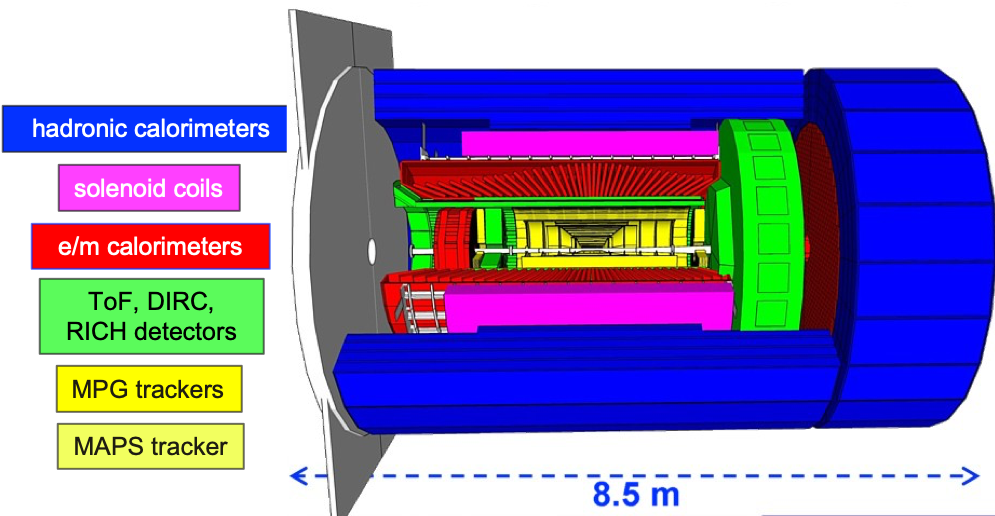
\includegraphics[width=0.9\textwidth]{figures/epic.png}
    \caption[Schematic view of the ePIC detector]{Crosscut view of the ePIC detector planned to be built at the EIC. Taken from Ref.~\cite{EIC}.}
    \label{df3}
\end{figure}
\FloatBarrier
The design of such detector focuses on tracking and vertexing, particle identification, calorimetry systems and endcap detectors \cite{EICdetectorrequirements}. Tracking and vertexing will be done using a double-sided time projection chamber, gas electron multipliers (GEM), $\mu$MEGA, that can be used for tracking neutrons, or $\mu$RWELL (more in Ref.~\cite{muWELL}) which all are high precision gas detectors. At the moment, the best material for vertex tracking is silicon, which is why all the tracking detectors will be made from this material \cite{Higinbotham}. Particle identification relies highly on ionization trails from TPC, but there will be additional detectors which are based on the principle of Cherenkov radiation such as a dual and modular Ring Imaging Cherenkov Detector (dRICH and RICH) and internally reflected Cherenkov light detectors \cite{EICdetectorrequirements}. The measurement of energy of particles will be provided through electromagnetic (ECAL) and hadron (HCAL) calorimeters. The exact types with specific properties are still under study. In addition to the detector of the central region, auxiliary detectors for forward and backward regions will be installed. Roman pots for far-forward tagging, ZDCs for detecting neutrons and low-energy photons will be installed as well as some other detectors that have not been chosen yet. Polarimeters, detectors that measure polarization, will be installed in several sections of the EIC \cite{EICdetectorrequirements}. All of the detectors which will be part of the Electron-Ion Collider are currently being tested at Thomas Jefferson National Accelerator Facility. Jefferson lab is another laboratory under the administration of U.S. Department of Energy and is located in Virginia, U.S. EIC is expected to begin running in the early 2030s.
  % STAR & RHIC
\newpage
\chapter{Event selection and particle identification}
\label{analysis}
This chapter discusses the selection of events based on their relevance for this thesis. At the beginning of this chapter, the conversion of signal to actual data files is discussed. Following, the event selection and individual cuts will be explained and reasoned. Last section of this chapter debates the conditions imposed on identifying particles. 
\section{Data sample}
\label{data}
Signals, that are measured by the detectors, are moved to Data Acquisition system (DAQ) to be processed. This involves readout and digitization which is facilitated by a Gigalink with the speed of 80 Mb/event, pedestal subtraction, creation of events and lastly moving the data to RHIC Computing Facility (RCF). The transfer is accommodated through a Gigabit ethernet with the speed of 100 Mb/s \cite{DAQ}. Files are saved in the MuDst (MicroDST) format. Essentially, MuDst are ROOT files\cite{ROOT} which include a tree with branches that contain all the information about the events. MuDst files are incredibly large files which contain information and data which is often redundant. That is why a different format is used: PicoDst. PicoDst involves all the necessary data needed and is much more practical. The official framework that has the PicoDst format and involves data from Roman Pot system is called \textit{star-upcDst}.  
\newline
Data taking for this analysis was part of Run17 which happened in 2017. The collisions were proton-proton at center of mass energy $\sqrt{s}=510$ GeV. The analysis was done using the ROOT framework developed by CERN for analysing large data files. The analysis was computated using the RHIC Computing Facility.


\section{Event selection}
This section discusses all the different conditions imposed on measured events to separate the relevant ones. At the beginning, the data set involves $2.03\cdot10^9$ events. \autoref{af1} shows the different cuts and the progress in number of events selected. Different graphs are provided for the different conditions throughout the section. First part explains the Central Production Trigger, then the conditions regarding the forward scattered protons and in the end the hadrons produced in the central system. The distributions shown in this section include data that passed the condition before and show the representation of cuts in black dashed line.

\FloatBarrier
\begin{figure}[ht]
    \centering
    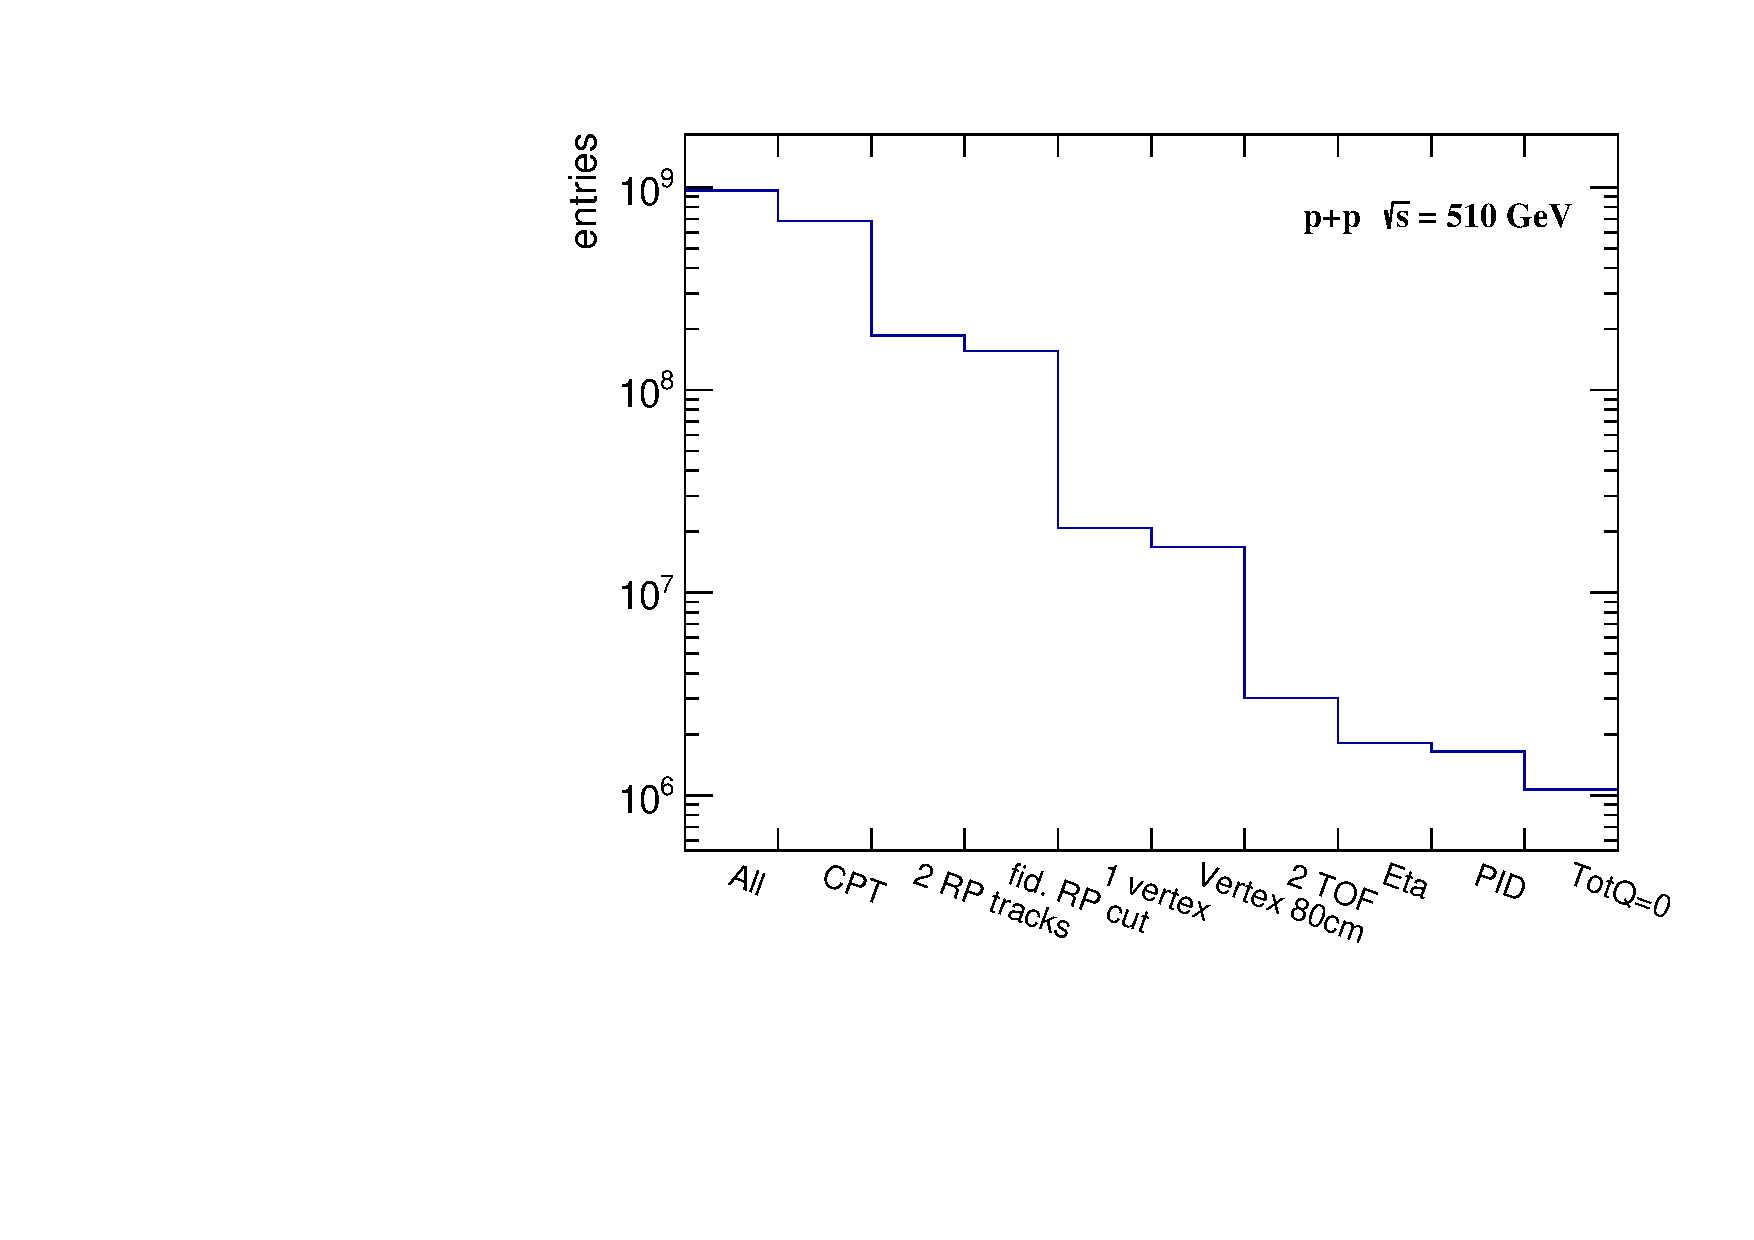
\includegraphics[width=1\textwidth]{figures/AnalysisFlow.pdf}
    \caption[Event selection for production of $K^0_S$ and $\lambda^0$]{Histogram of number of events that pass different cuts.}
    \label{af1}
\end{figure}
\FloatBarrier

\subsection{Central Production Trigger}

\FloatBarrier
\begin{table}[ht]
    \centering
    \begin{tabular}{c|c|c}
    
        condition &  & \\ \hline
       Elastic combination of hits in RP & - & + \\ 
       Inelastic combination of hits in RP & + & - \\
       Number of hits in TOF >1 & + & + \\
       Number of hits in TOF <10 & - & - \\
       Hit in BBC east & - & - \\
       Hit in BBC west & - & - \\
       Hit in BBC Large east & - & -\\
       Hit in BBC Large west & - & - \\
       Hit in ZDC east & - & -\\
       Hit in ZDC west & - & - \\
    \end{tabular}
    \caption[Table of conditions for Central Production Trigger]{Table of conditions Central Production Trigger is comprised of.}
    \label{at38}
\end{table}
\FloatBarrier
The first cut on events is provided by the Central Production Trigger (CPT). All the different conditions this cut involves are listed in \autoref{at38}. First 2 conditions are regarding combinations of hits in Roman Pots. Elastic combination means one proton on each side but one is Up and one is Down. Inelastic combination means on both sides Up or both Down as was discussed in \autoref{STAR}, \autoref{RPs}. Next 2 conditions require  multiplicity in Time Of Flight detector to be between 2 and 10. The rest of the conditions listed regard detectors BBC and ZDC. Beam Beam Counters cover pseudorapidity regions of $3.3<\eta<5$ and Zero Degree Calorimeters are located behind dipole magnets at level of interaction point. The reason for these conditions is to ensure large gaps in rapidity on each side which are distinctive features of diffractive events.
\subsection{2 Roman Pot tracks}

\FloatBarrier
\begin{figure}[ht]
    \centering
    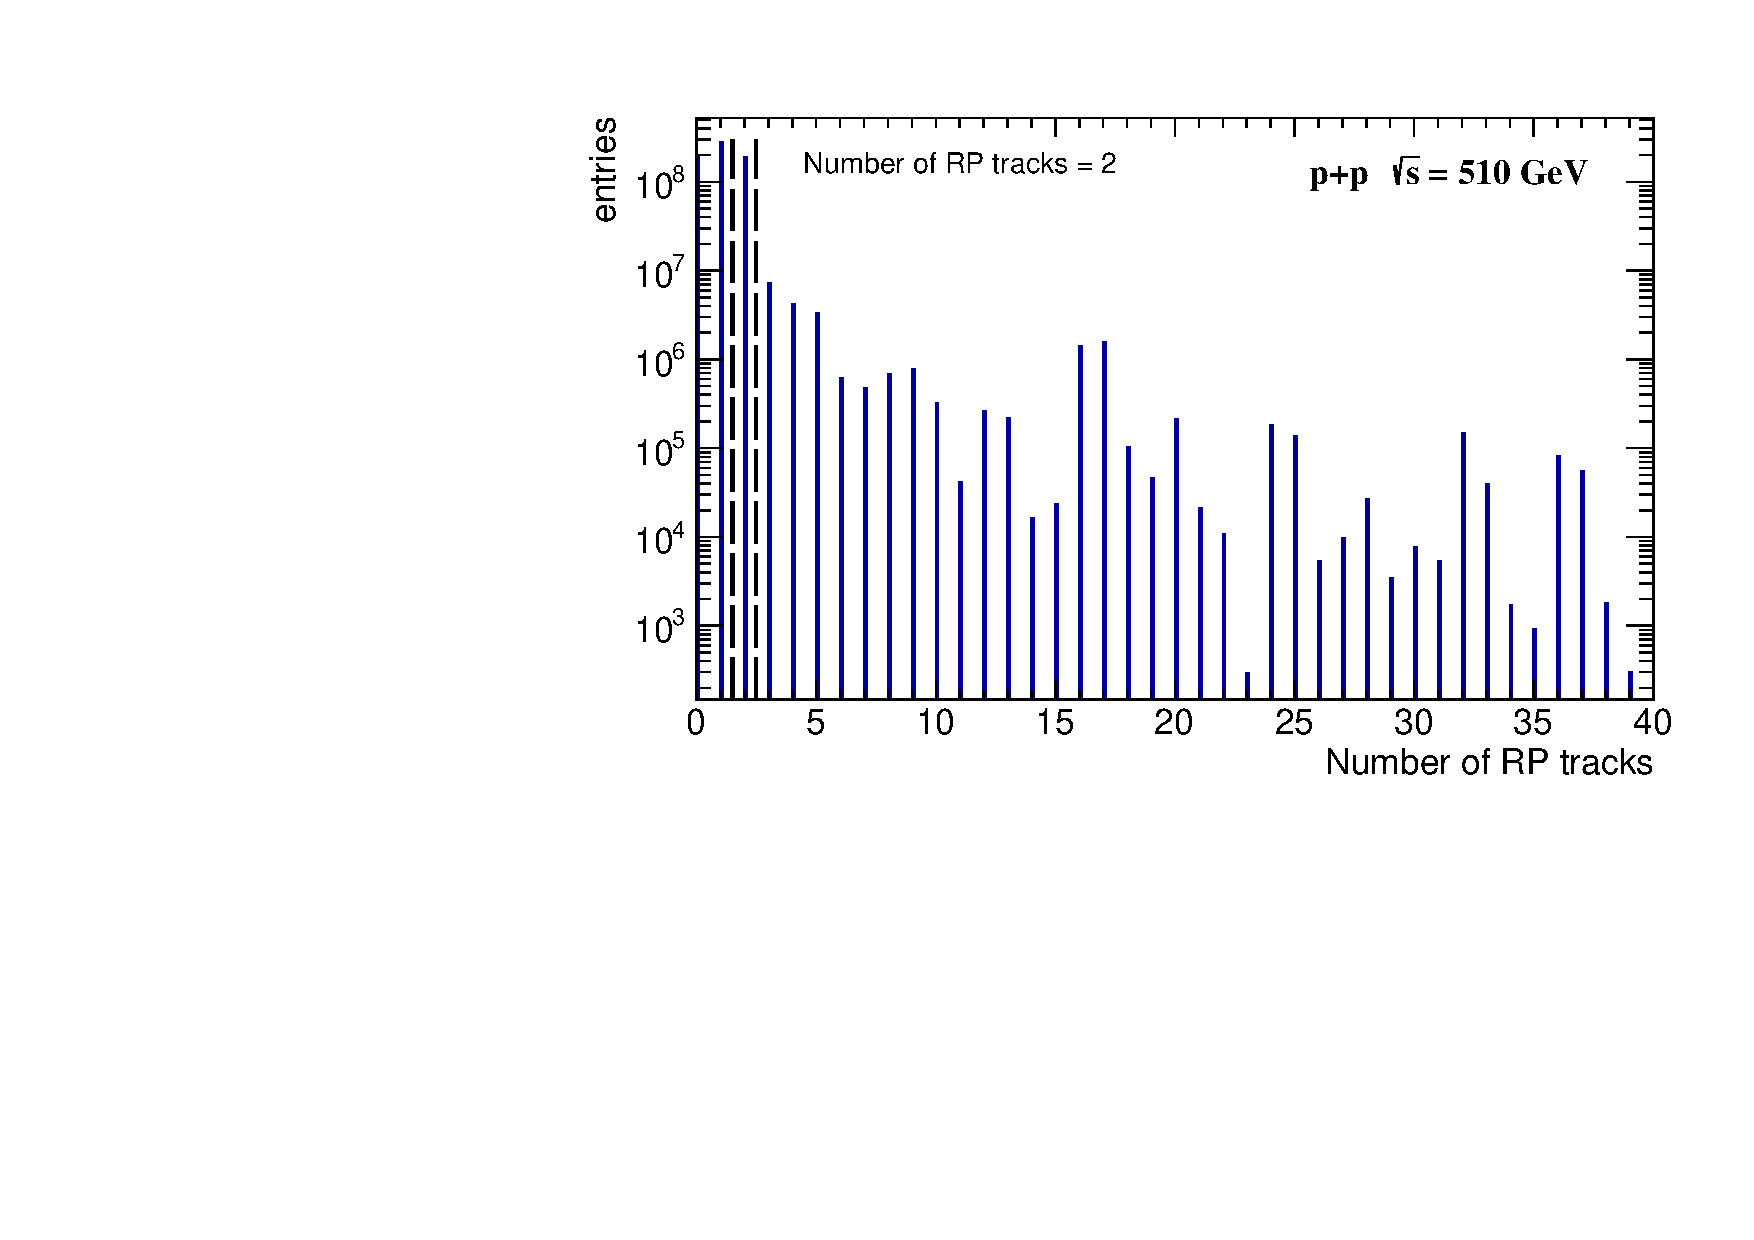
\includegraphics[width=1\textwidth]{figures/NumberRPTracks.pdf}
    \caption[Distribution of number of tracks in Roman Pot system]{Distribution of number of tracks in Roman Pots. The only allowed number is one on the west and one on the east side of the detector.}
    \label{af2}
\end{figure}
\FloatBarrier
The second condition for event selection is that for each event, 2 proton tracks must be registered. Their positions are also important. One track has to be on each side (east or west) of the detector as can be seen in \autoref{df6}. Part of this condition is also the necessity that 3 out of 4 Silicon Strip Detectors inside a Roman Pot have to register a particle. This ensures a certain level accuracy for momentum measurement. The histogram of number of RP tracks per event can be seen in \autoref{af2}. 
\subsection{Fiducial Roman Pot cut}
This next cut focuses on the position of forward protons in transverse plane detected in Roman Pots. To ensure good quality of reconstruction of proton momentum, all the SSD detectors in RPs, that registered a proton, are involved. The fiducial region is estimated to have high geometric acceptance, track reconstruction efficiency and it minimizes the systematic uncertainties\cite{Truhlar}. The fiducial region is defined by the following conditions.
\begin{gather*}  
(p_x + 0.6~\textrm{GeV})^2 + p_y^2 < 1.25 \textrm{ GeV}^2\textrm{/c}^2 \\
0.4 \textrm{ GeV/c } < |p_y| < 0.8 \textrm{ GeV/c} \\
p_x > -0.27 \textrm{ GeV/c}
\label{ea1}
\end{gather*}
\FloatBarrier
\begin{figure}[ht]
    \centering
    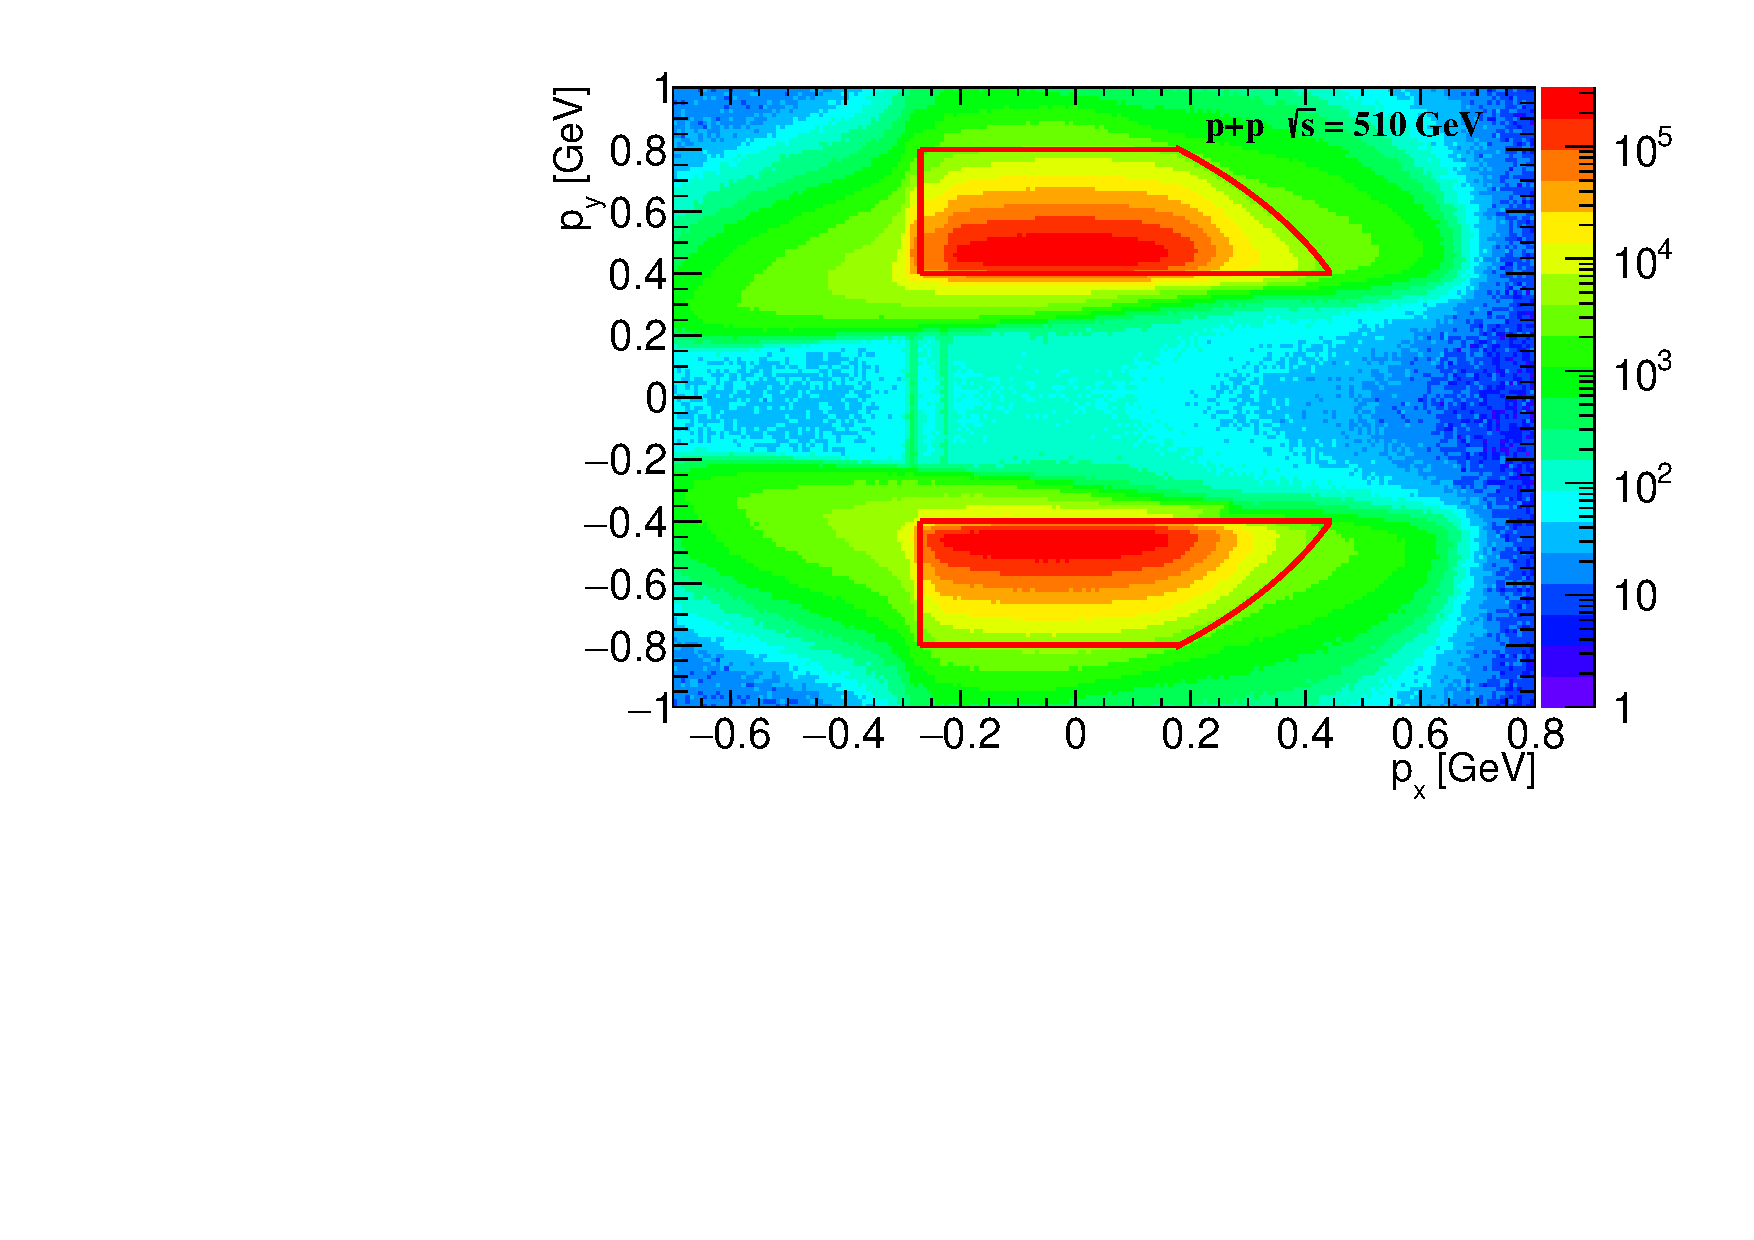
\includegraphics[width=1\textwidth]{figures/hRPcorr.pdf}
    \caption[Correlation graph of transverse momentum in Roman Pot system]{Correlation graph of transverse momenta of scattered protons. Red lines define the fiducial region in Roman Pots.}
    \label{af3}
\end{figure}
\FloatBarrier
The following 2 graphs show the same data but only they are differentiated based on the side where they were measured. Graphs do show a slight shift between the lines that represent the fiducial cut and the position of the structure in the middle. This shift is caused by the displacement of the detectors on the east side by 3 mm. 

\FloatBarrier
\begin{figure}[ht]
    \centering
    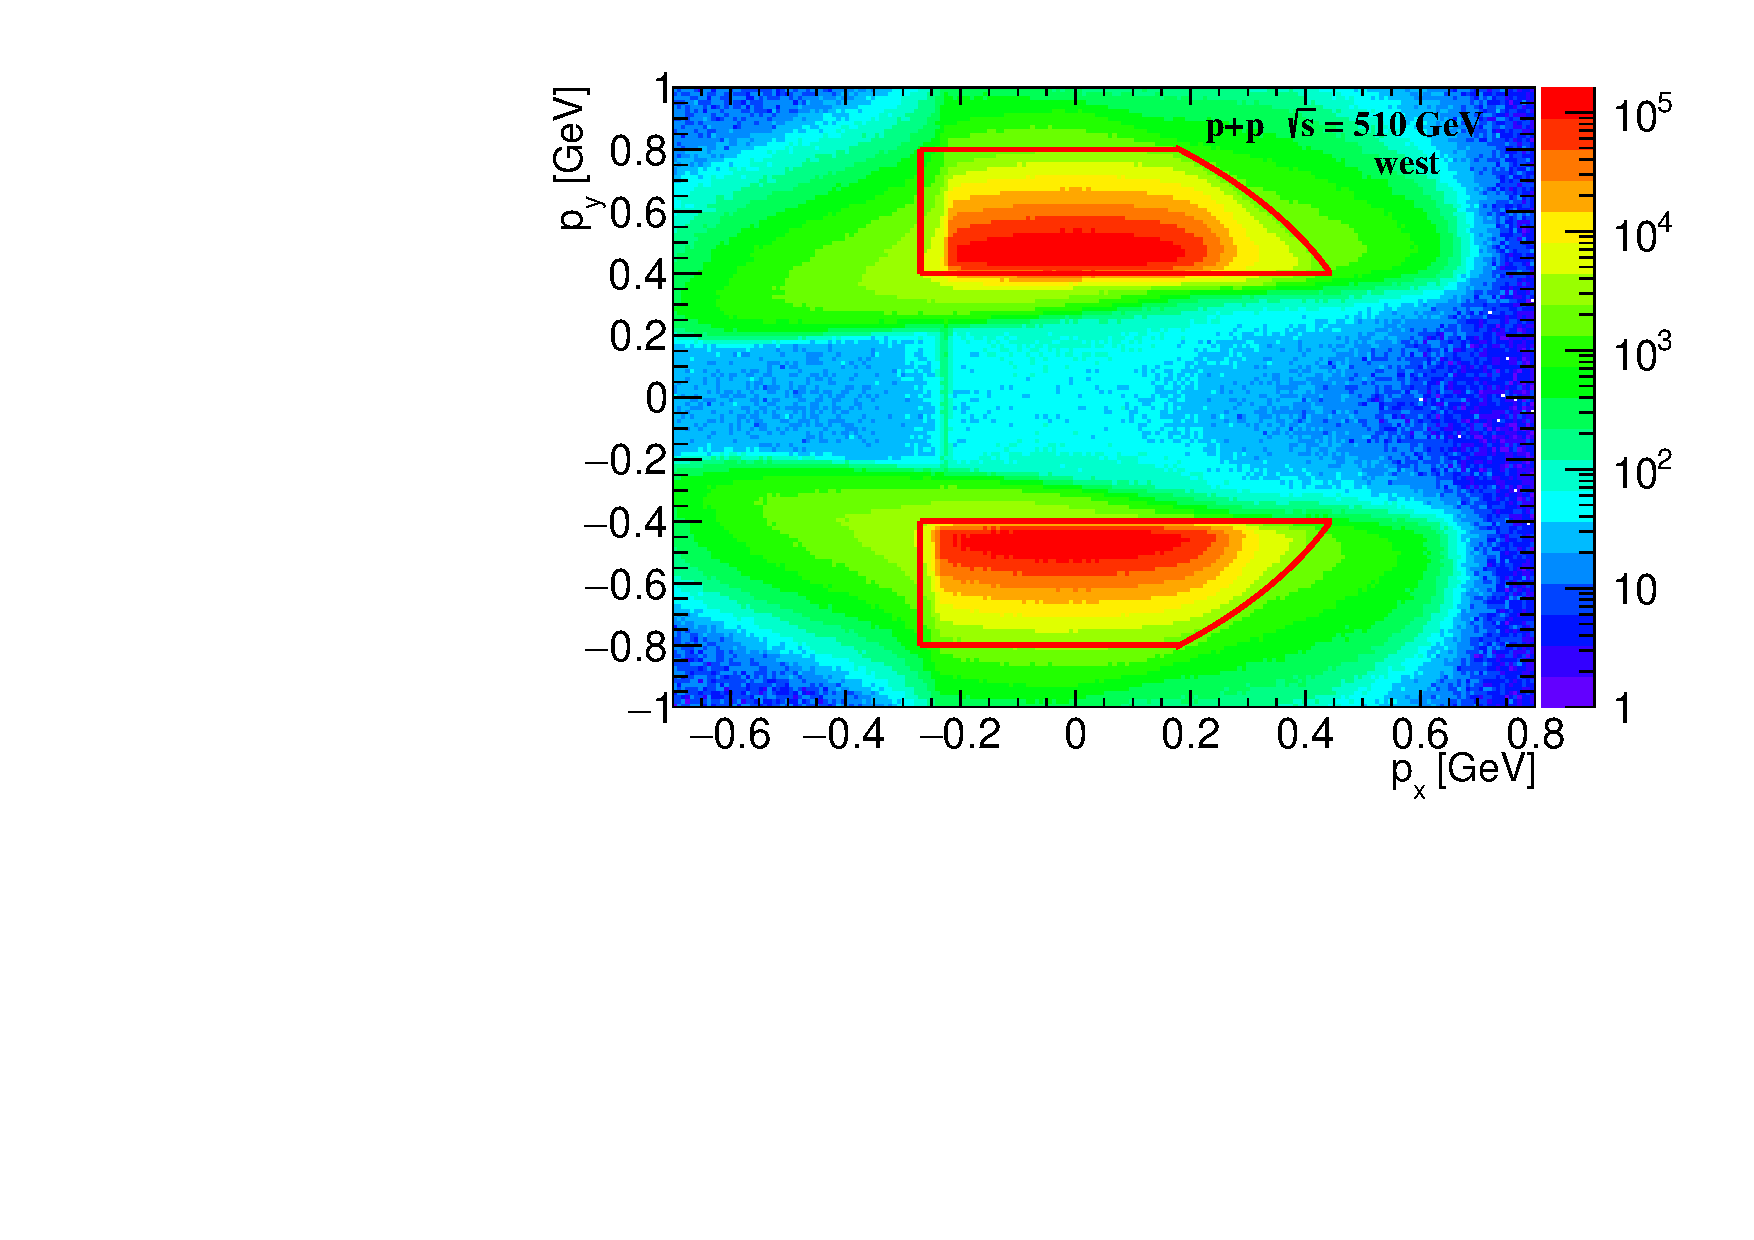
\includegraphics[width=1\textwidth]{figures/hRPcorrWest.pdf}
    \caption[Correlation graph of transverse momentum in Roman Pot system on the west side of the detector]{Correlation graph of transverse momentum in Roman Pot system on the west side of the detector.}
    \label{af4}
\end{figure}
\FloatBarrier

\FloatBarrier
\begin{figure}[ht]
    \centering
    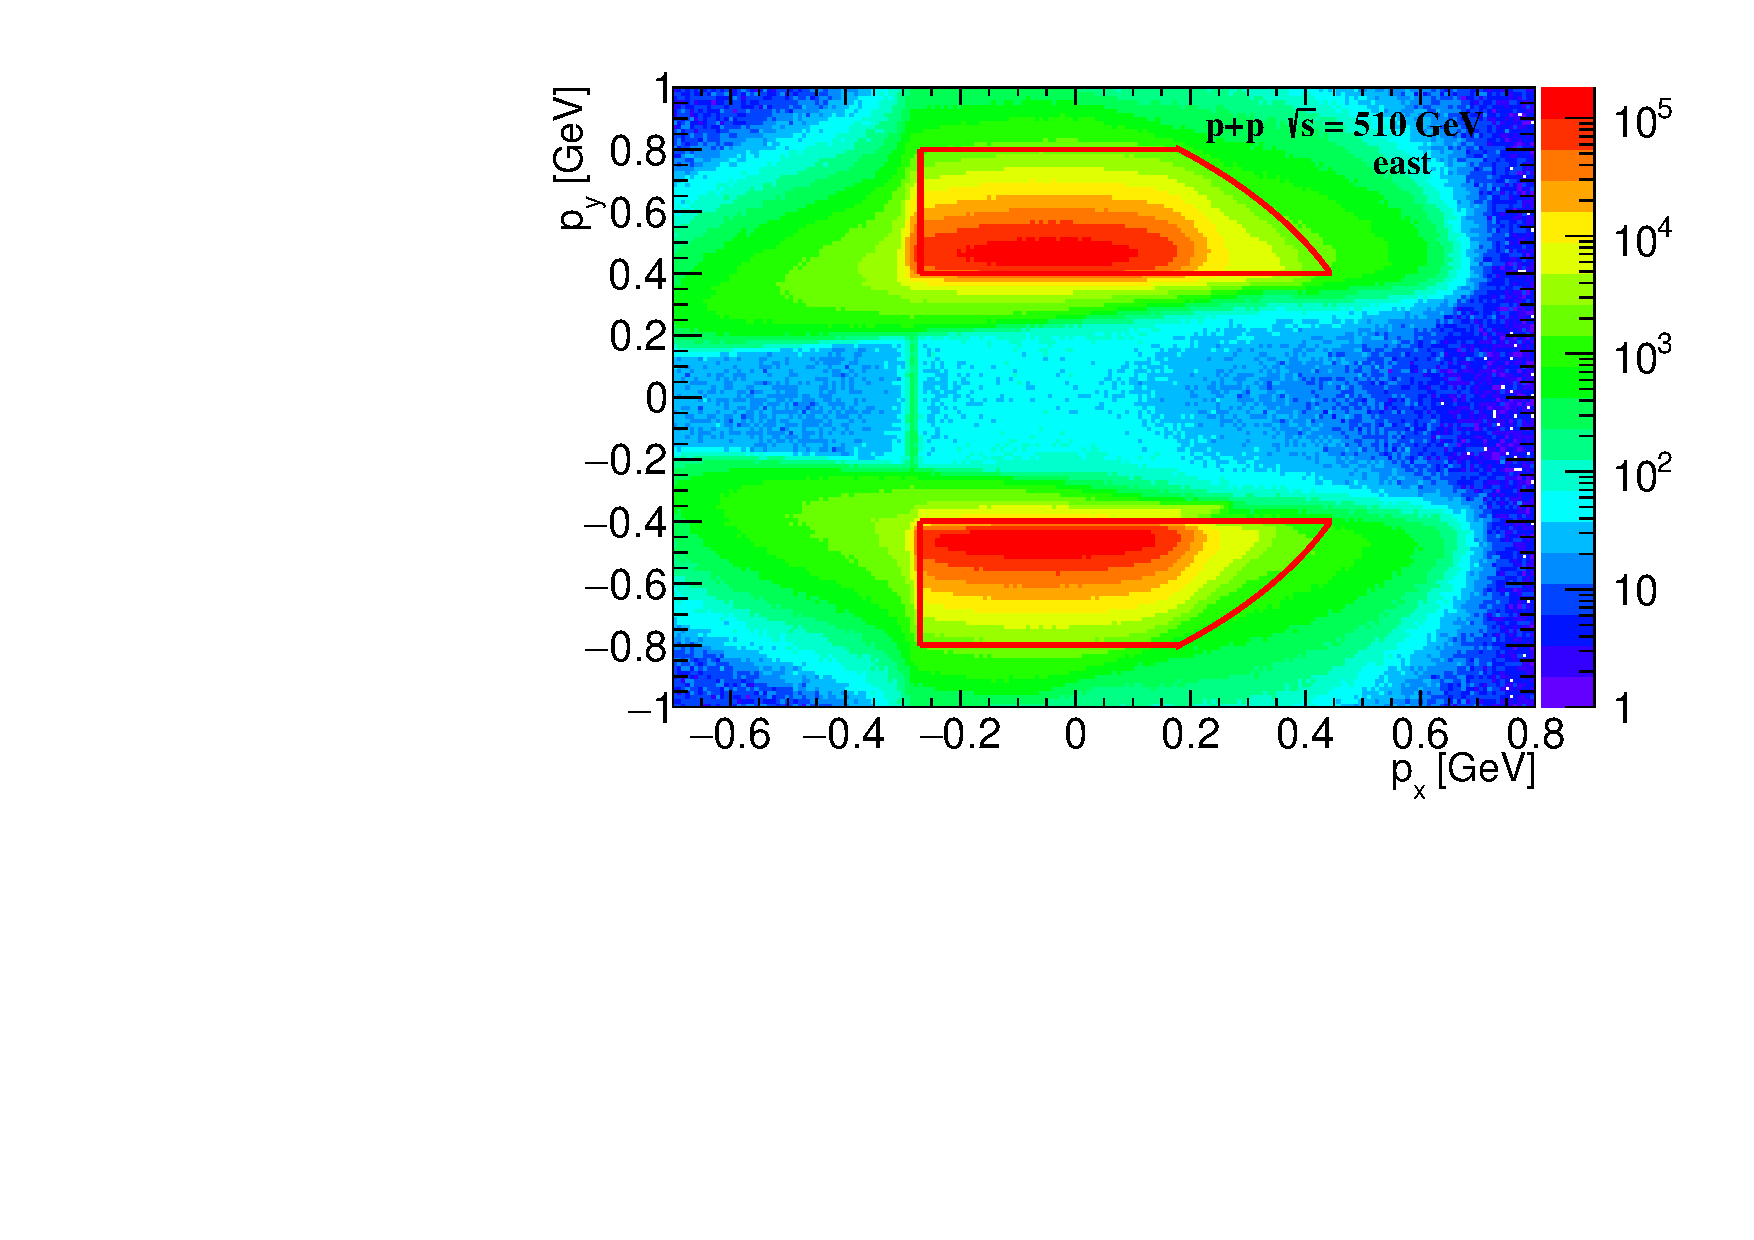
\includegraphics[width=1\textwidth]{figures/hRPcorrEast.pdf}
    \caption[Correlation graph of transverse momentum in Roman Pot system on the east side of the detector]{Correlation graph of transverse momentum in Roman Pot system on the east side of the detector.}
    \label{af17}
\end{figure}
\FloatBarrier
\subsection{Number of vertices}
\label{posZ}

\FloatBarrier
\begin{figure}[ht]
    \centering
    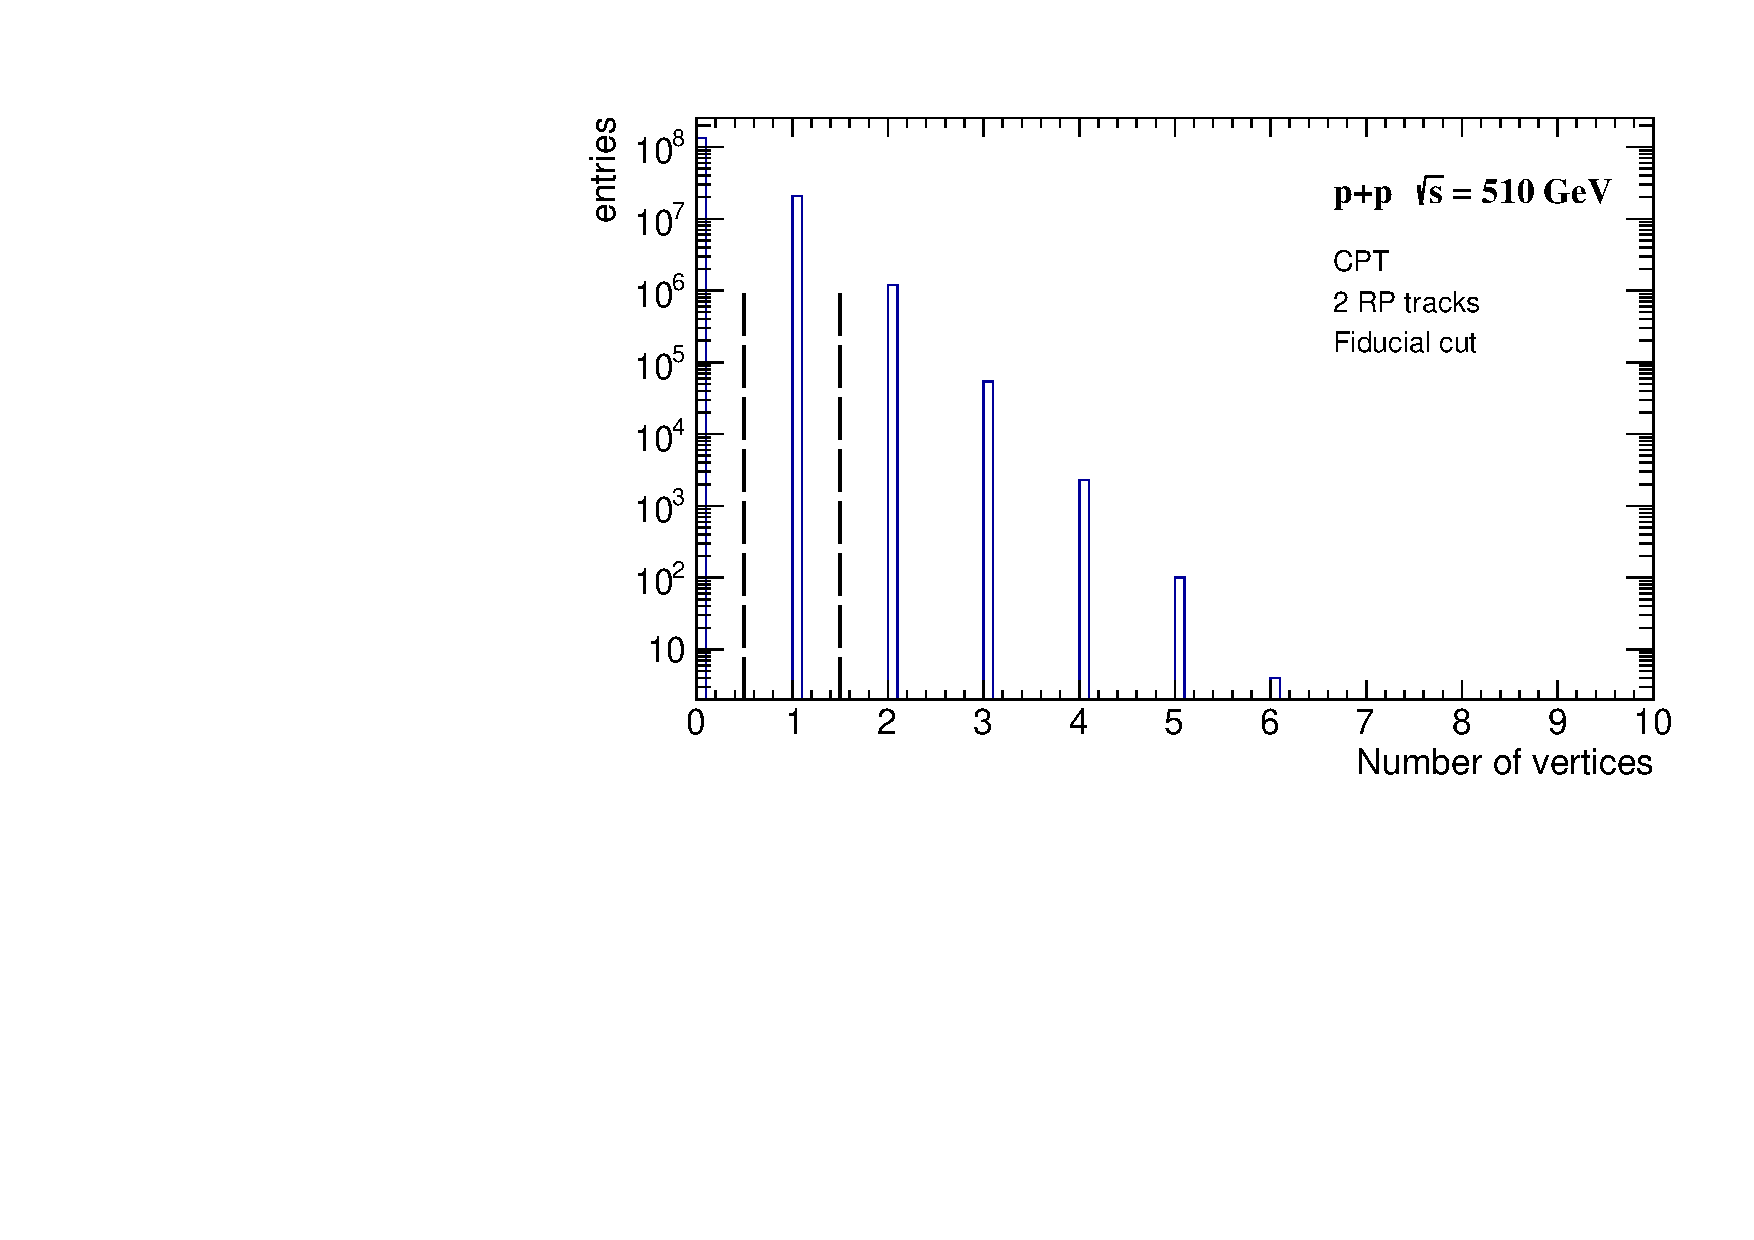
\includegraphics[width=1\textwidth]{figures/hNVertices.pdf}
    \caption[Distribution of number of vertices in the central tracking system]{Distribution of number of vertices in the central tracking system. The y coordinate is logarithmic scale.}
    \label{af69}
\end{figure}
\FloatBarrier

Moving on to central tracking system, the first condition is imposed on number of vertices. The condition is to have 1 and only 1 vertex. The position of vertex is reconstructed from the particle tracks in TPC. To be exact, the reconstructed vertex for the processes that are interesting for this thesis is not the primary but the secondary vertex of the event where the measured neutral particle decays into the hadron pair. The position of primary vertex is not known due to the small number of tracks. The primary vertex of the event would be located less than $3$ cm and $8$ cm away from the secondary vertex for $K^0_S$ and $\Lambda^0$ respectively\footnote{If we consider the PDG values \cite{zyla} for lifetimes to be $8.954 \pm 0.004$ $10^{-11}$ s ($K^0_S$) and $2.63 \pm 0.02$ $10^{-10}$ s ($\Lambda^0$) and that they move with the speed of light $c=2.999~792$ m/s, then the distance travelled will be around the previously mentioned values.}. The distribution of number of vertices can be seen in \autoref{af69}.
\subsection{Vertex position of z coordinate}
 Another condition regards the position of z coordinate of vertex. For an event to pass the condition, it's vertex has to satisfy $|z_{vertex}| < 80$ cm from the interaction point which is the absolute middle of the detector. The reason for this condition is to have the best acceptance, effectiveness and 
to minimize the systematic errors.
\FloatBarrier
\begin{figure}[ht]
    \centering
    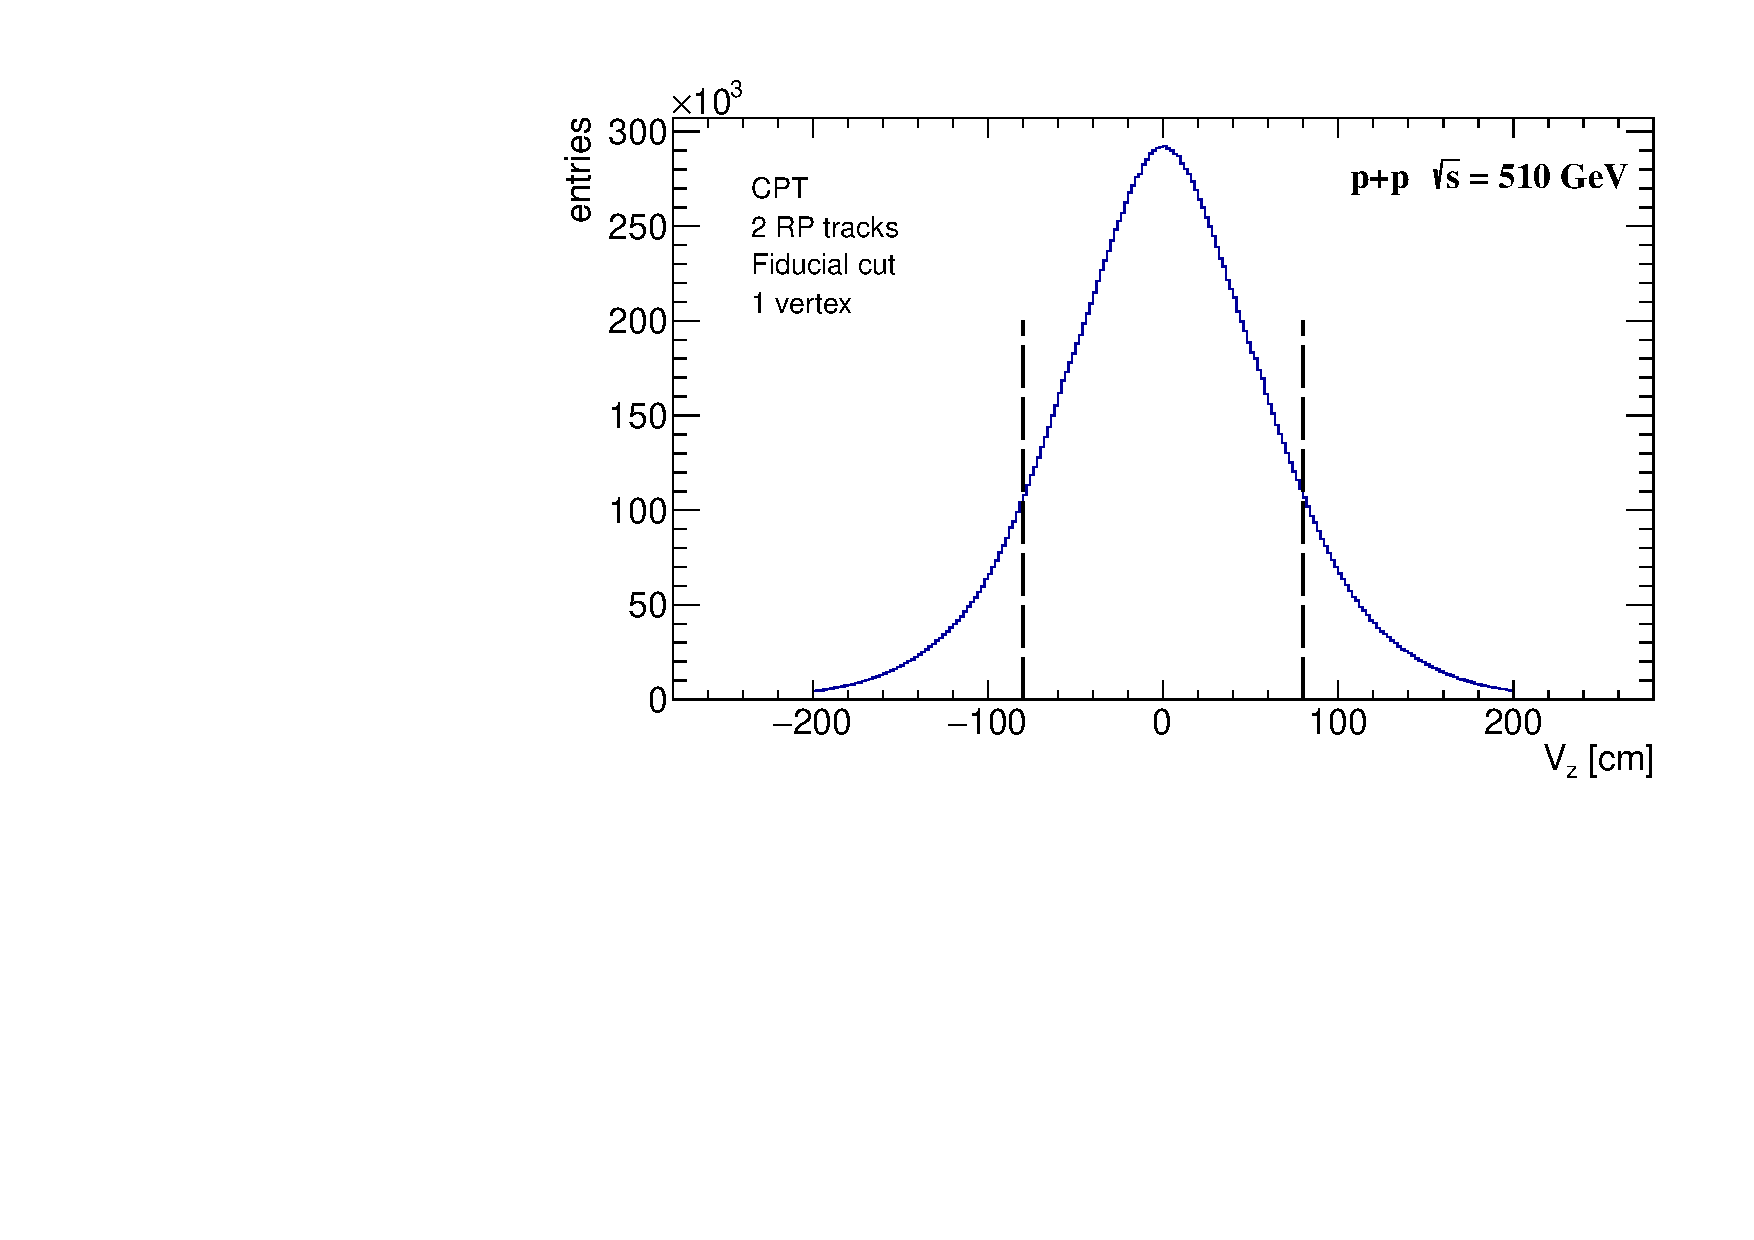
\includegraphics[width=1\textwidth]{figures/hPosZ.pdf}
    \caption[Distribution of z coordinate position of vertex]{The graph of distribution of z coordinate of vertex. Events that satisfy the condition $|z_{vertex}| < 80$ cm are selected.}
    \label{af5}
\end{figure}
\FloatBarrier
\subsection{2 tracks in TOF + other}
This next cut includes several conditions. The first condition is that only 2 hadron tracks per 1 event are allowed to be registered in the TOF detector. In addition, this condition allows studying exclusive events.
\newline
Another 2 conditions are based on the Distance of the Closest Approach (DCA) position. It is the distance between the closest point on the reconstructed track to the primary vertex. Because the position of the primary vertex of measured particles $K^0_S$ and $\Lambda^0$ is not known, the secondary vertex is assumed to be primary as it was mentioned in \autoref{posZ}. Framework \textit{upcDst} contains only primary tracks and not global, but the incorporation of global tracks is in progress. The conditions are separate for z coordinate and position in the transverse plane: $|DCA_z| < 1$ cm and $DCA_{xy} < 1.5$ cm and can be seen in \autoref{af6} and \autoref{af17}. 
\FloatBarrier
\begin{figure}[ht]
    \centering
    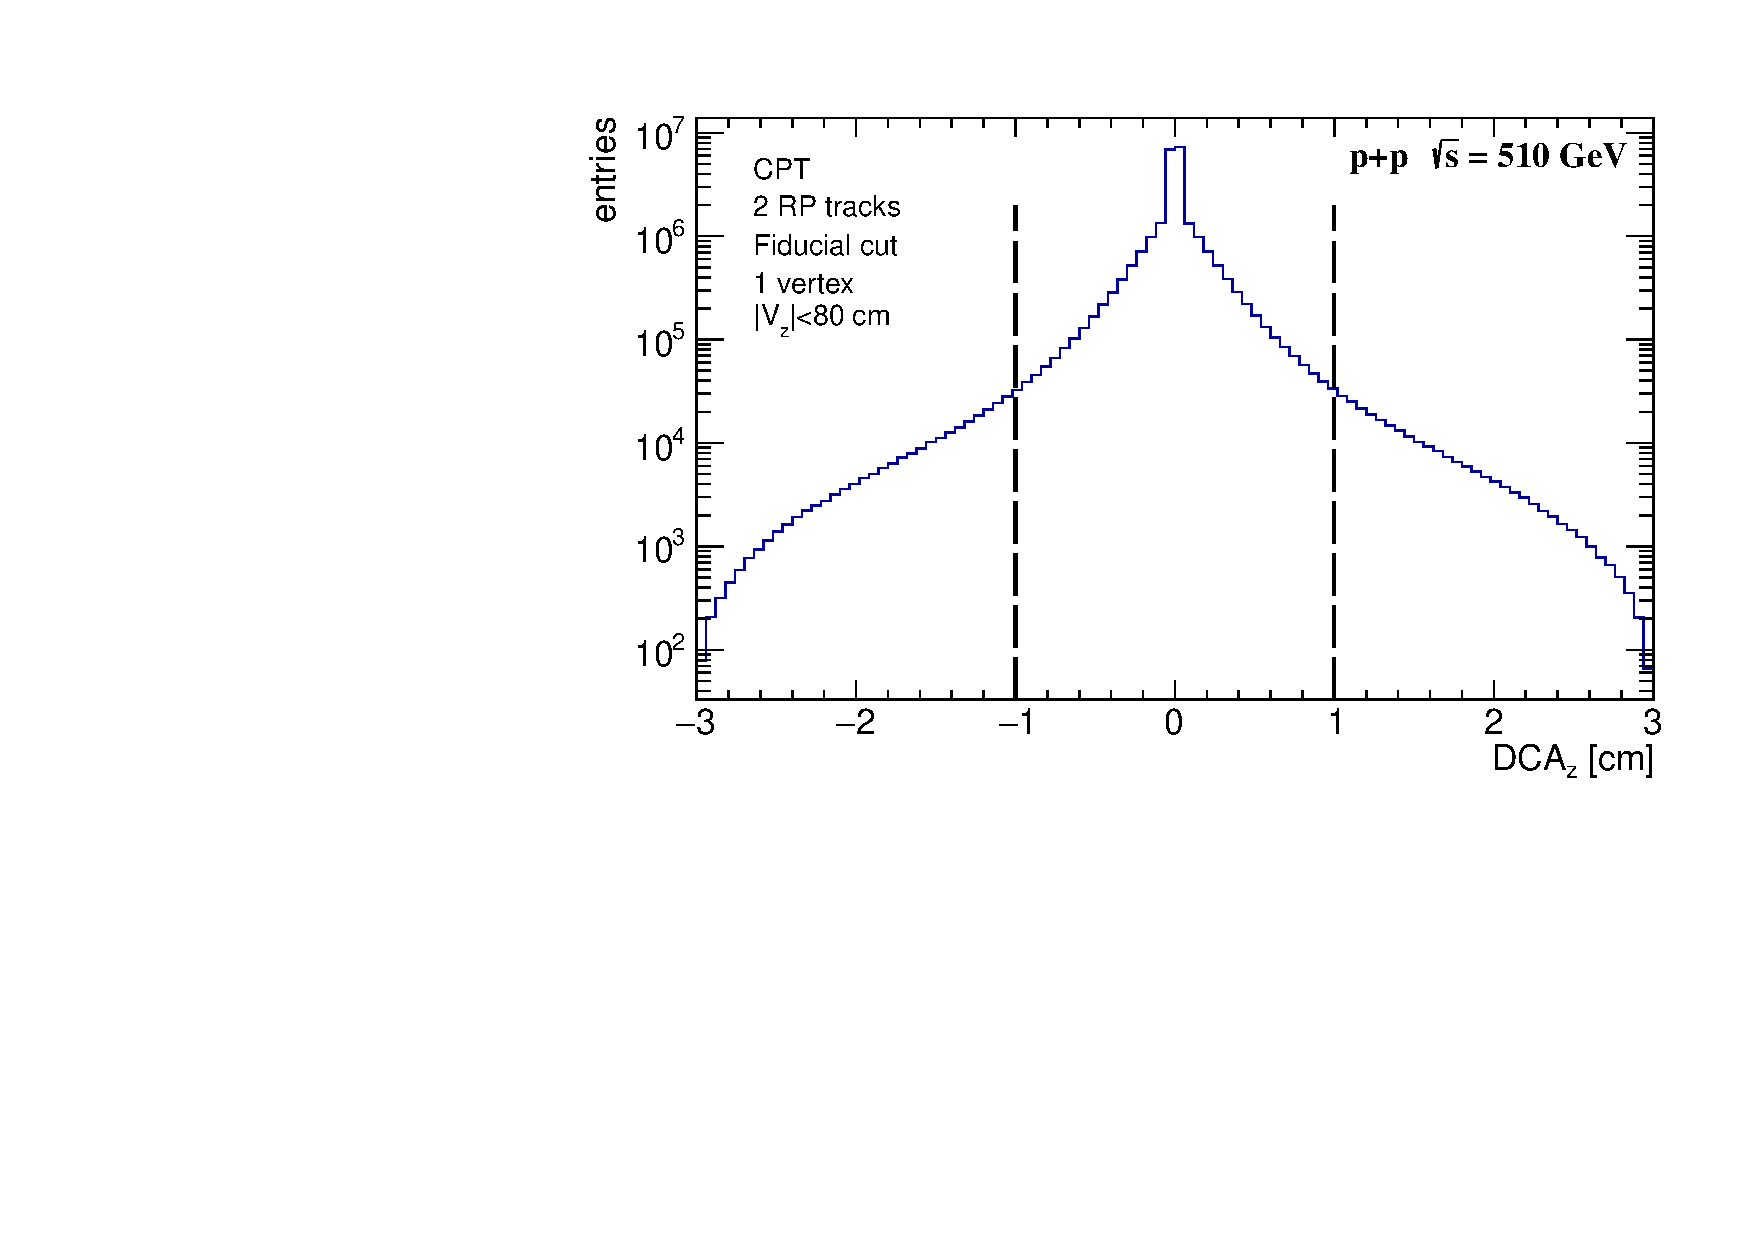
\includegraphics[width=1\textwidth]{figures/hDcaZ.pdf}
    \caption[Distribution of z coordinate of DCA]{Graph of distribution of DCA for z coordinate with logarithmic scale on vertical axis. The condition for z coordinate is $|DCA_z| < 1$ cm.}
    \label{af6}
\end{figure}
\FloatBarrier
\FloatBarrier
\begin{figure}[ht]
    \centering
    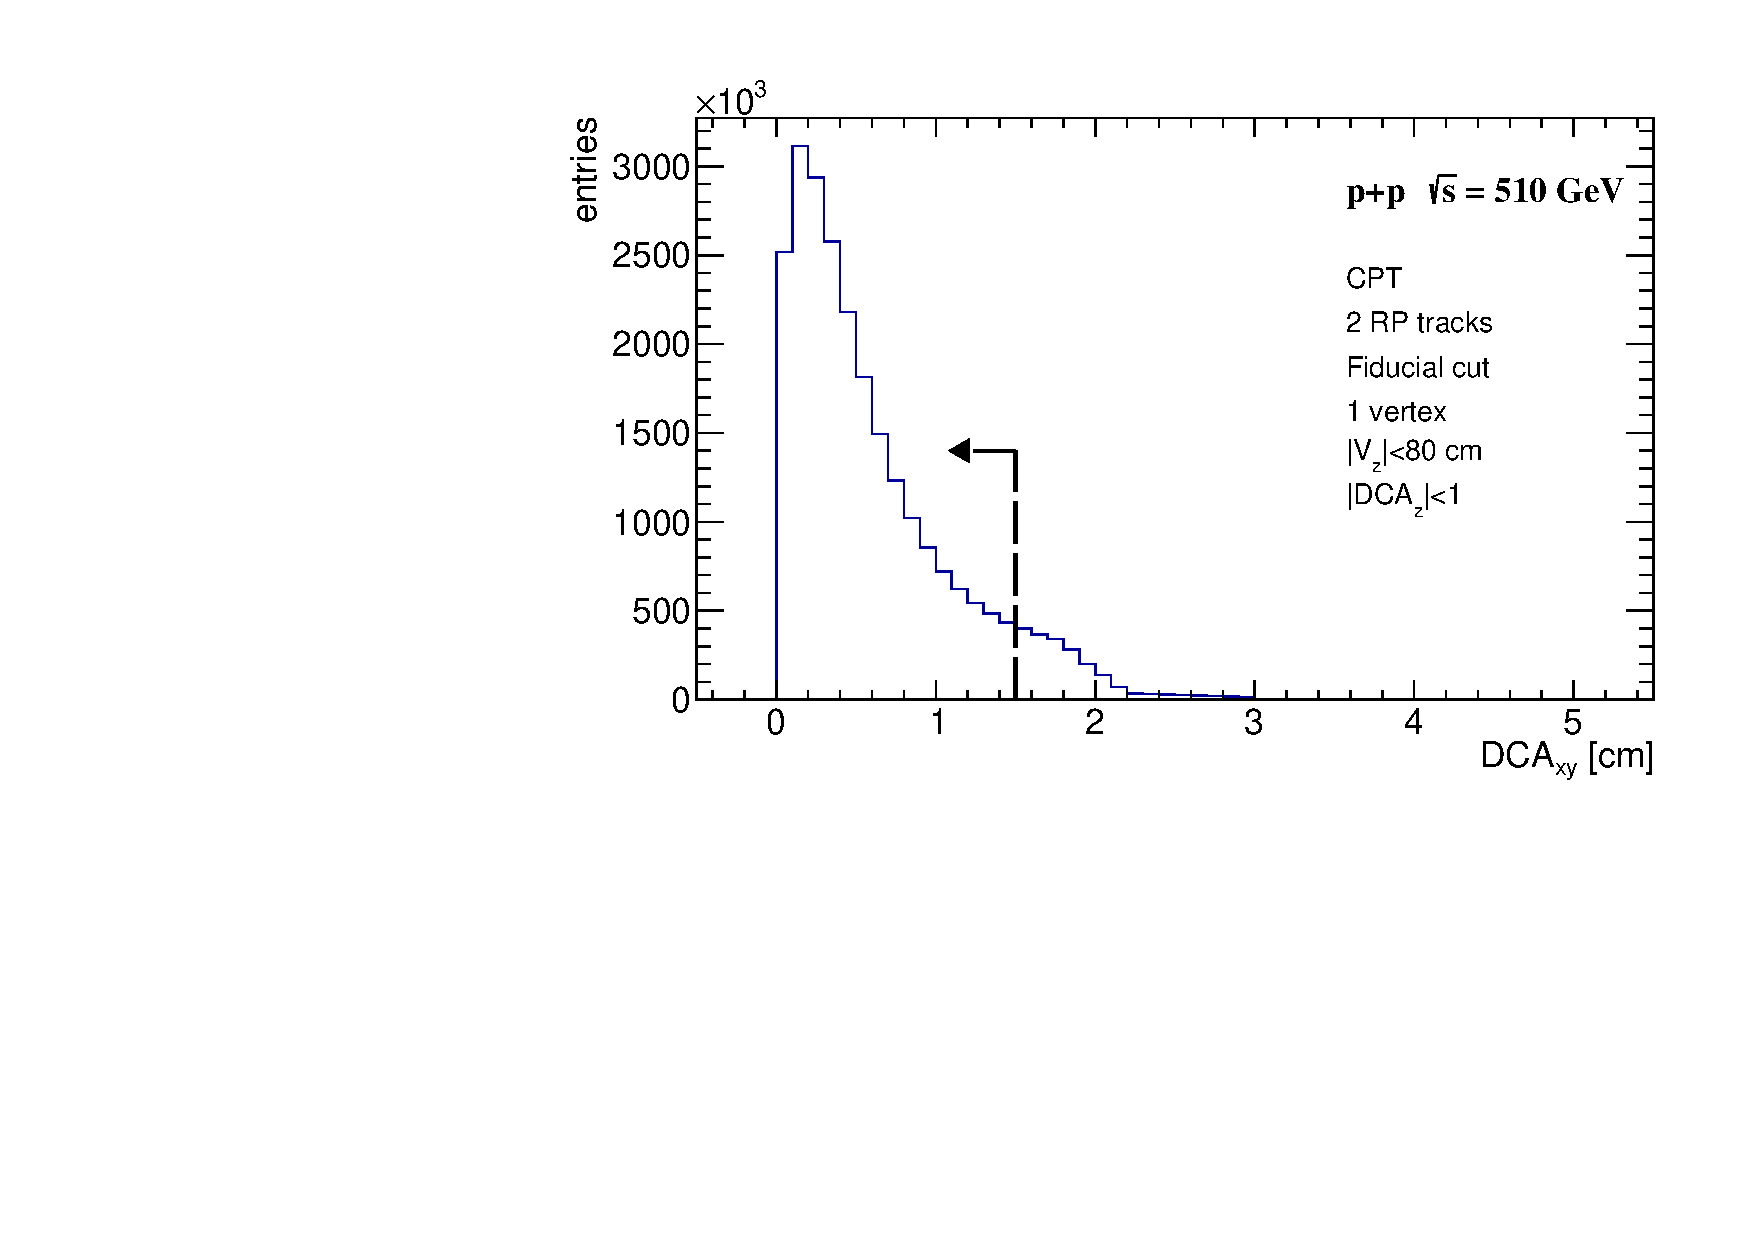
\includegraphics[width=1\textwidth]{figures/hDcaXY.pdf}
    \caption[Distribution of DCA $(x,y)$ plane] {Graph of distribution of DCA in the transverse plane $(x,y)$. Imposed condition is $DCA_{xy} < 1.5$ cm.}
    \label{af17}
\end{figure}
\FloatBarrier
Another 2 cuts are imposed on the number of hits in TPC. The bigger the number of hits is, the better is the resolution as it was described in \autoref{tpc}. For satisfactory track reconstruction and energy loss measurement numbers of hits 25 and 15 were required. Graphs for distributions can be seen in \autoref{af7} and \autoref{af16}. These are standard STAR conditions used at STAR.

\FloatBarrier
\begin{figure}[ht]
    \centering
    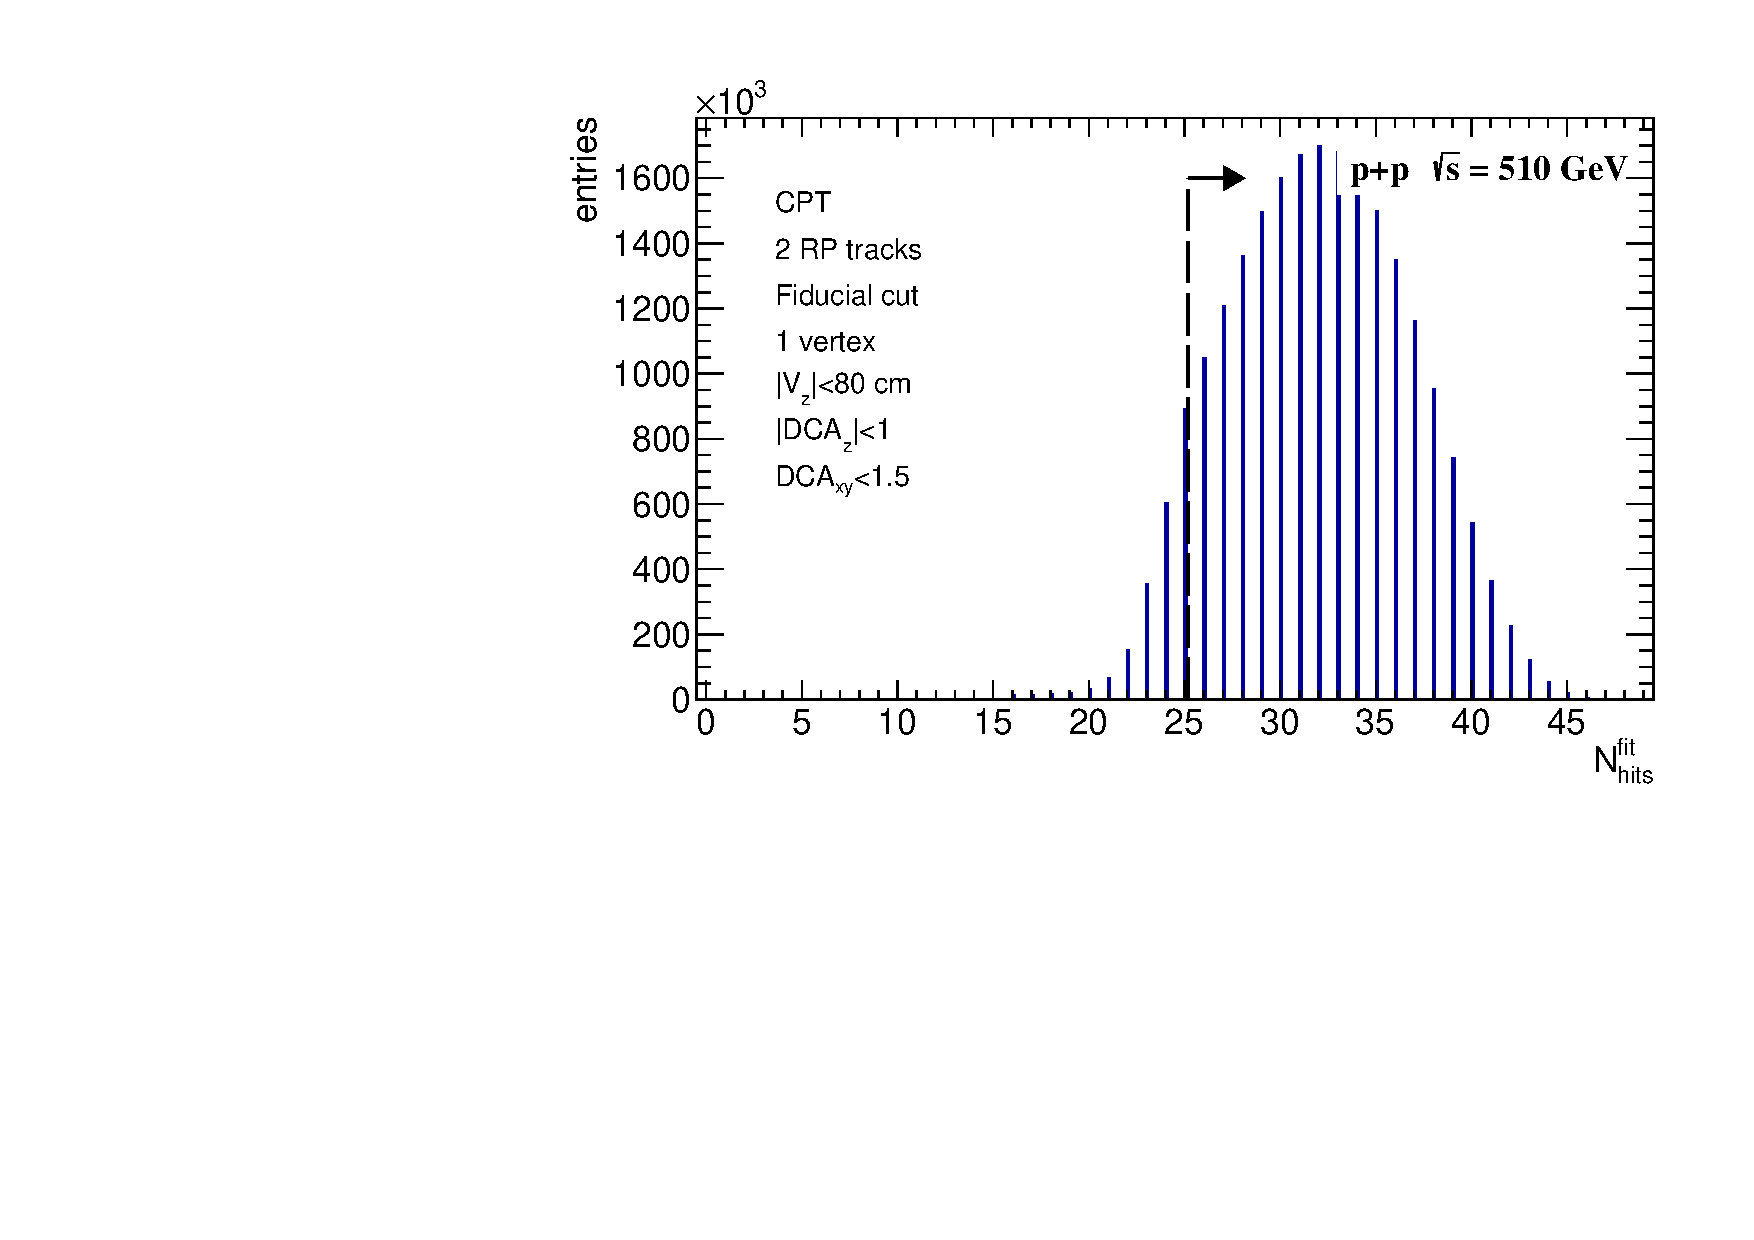
\includegraphics[width=1\textwidth]{figures/hNfitHits.pdf}
    \caption[Distribution of number of hits in TPC for track reconstruction]{Distribution of number of hits in TPC for track reconstruction.}
    \label{af7}
\end{figure}
\FloatBarrier

\FloatBarrier
\begin{figure}[ht]
    \centering
    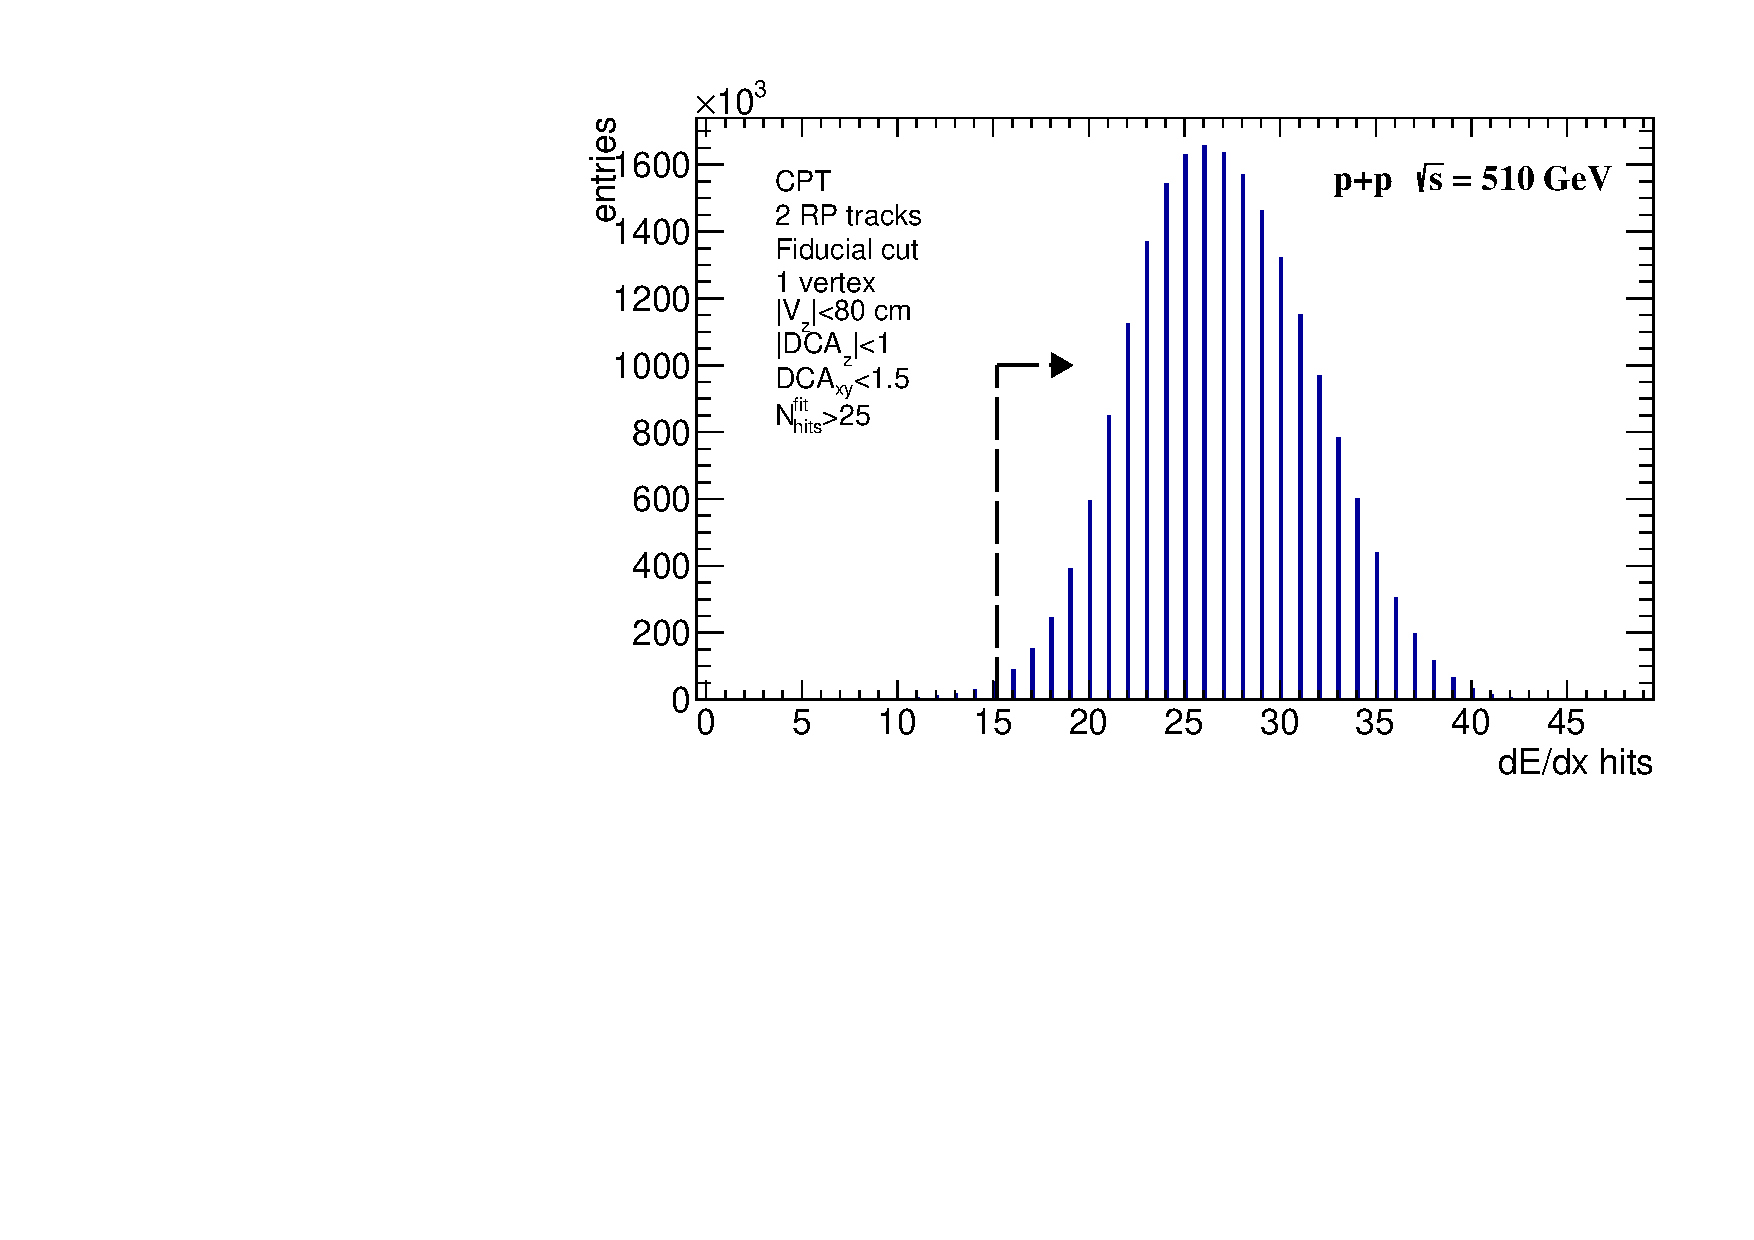
\includegraphics[width=1\textwidth]{figures/hNhitsDEdx.pdf}
    \caption[Distribution of number of hits in TPC for energy loss measurement]{Graph of distribution of number of hits for energy loss measurement.}
    \label{af16}
\end{figure}
\FloatBarrier

\subsection{Pseudorapidity}
The following condition considers the pseudorapidity of the scattered hadrons. Even though nowadays the acceptance of the TPC detector is quite high ($|\eta| < 1.5$) the measurement was done before the upgrade so the events chosen for the analysis have to satisfy the condition $|\eta|<0.7$. The reasoning behind this condition is that the hadrons have to be within the TOF acceptance. The pseudorapidity distribution and the imposed cuts can be seen in \autoref{af8}.

\FloatBarrier
\begin{figure}[ht]
    \centering
    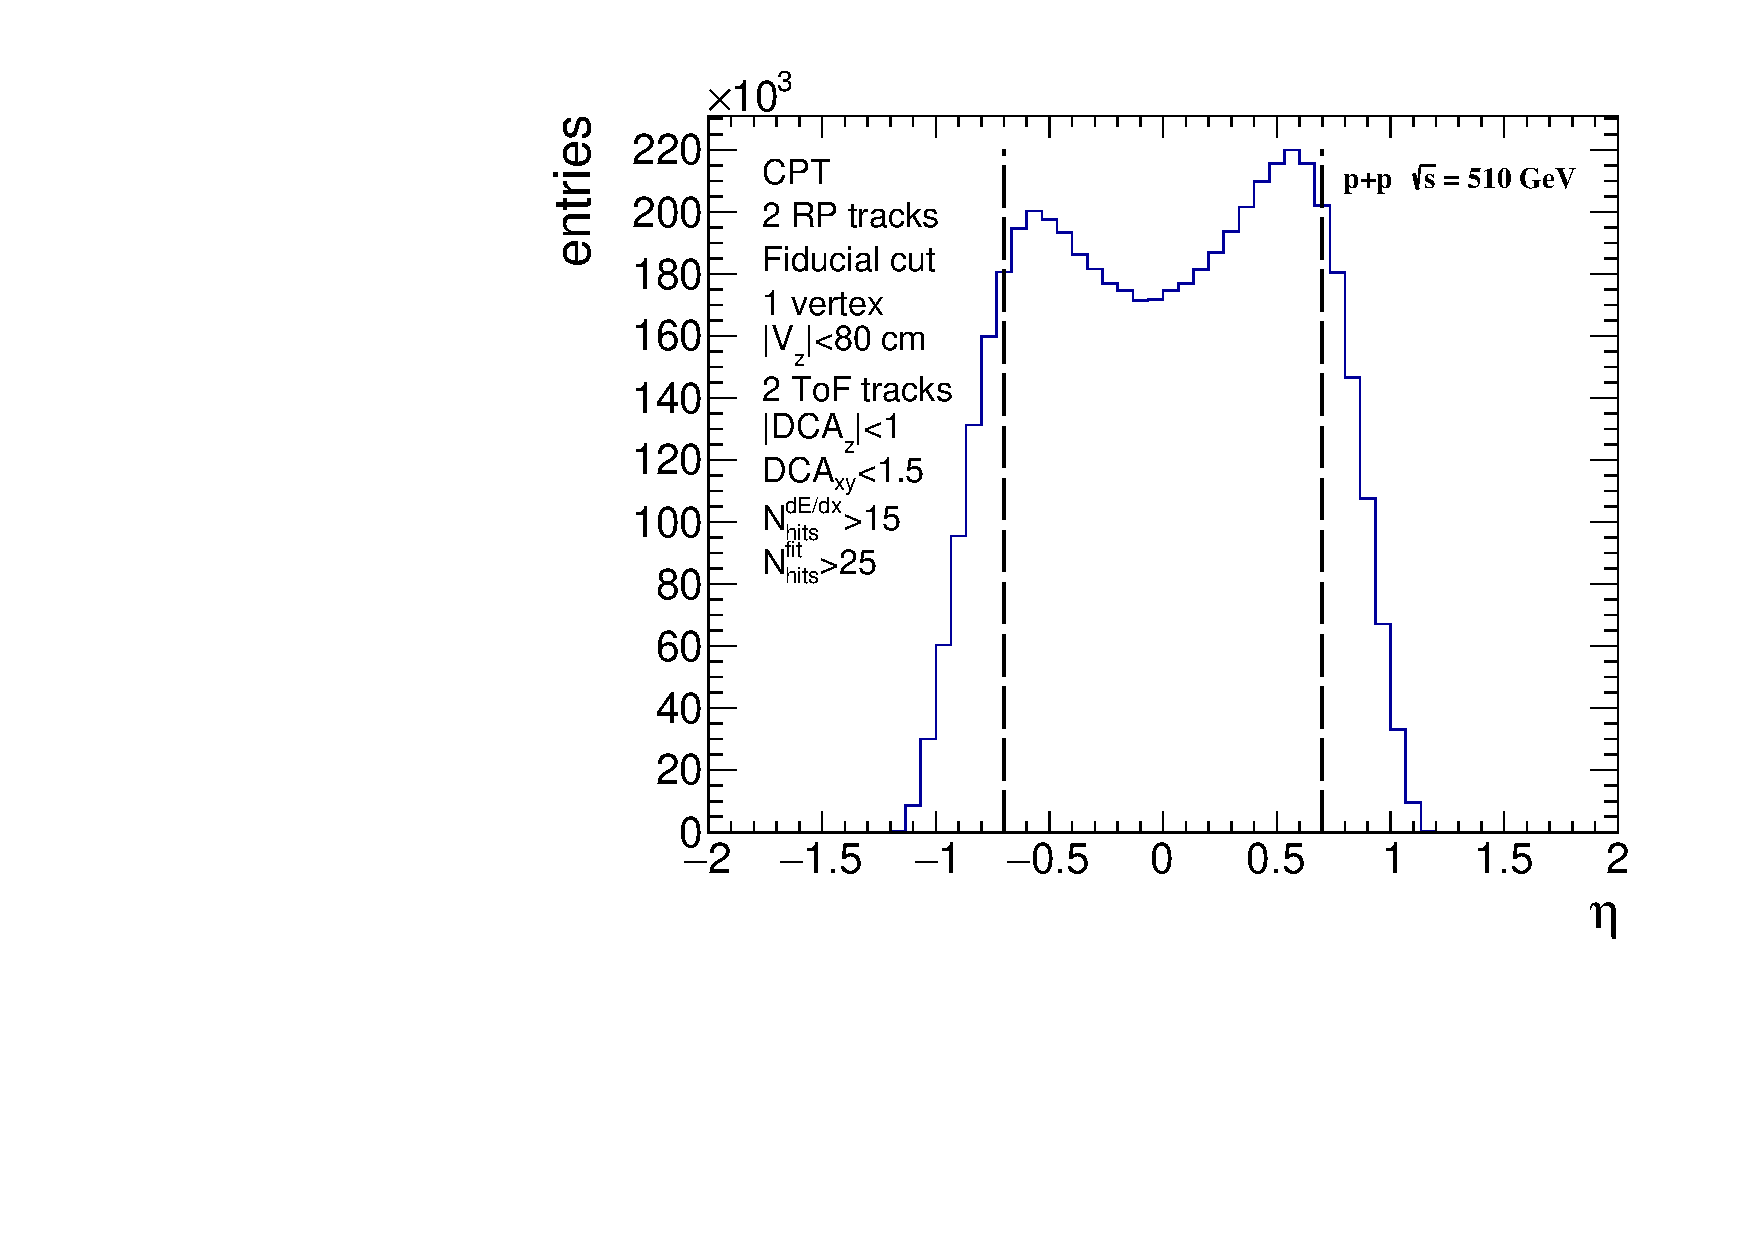
\includegraphics[width=1\textwidth]{figures/hEta.pdf}
    \caption[Distribution of pseudorapidity of measured hadrons]{Graph of distribution of pseudorapidity for created hadrons. The selected events must satisfy $|\eta| < 0.7$. }
    \label{af8}
\end{figure}
\FloatBarrier

\subsection{Total charge}
The last condition imposed on the selection of events is that the total charge of the created hadron pair has to be equal to 0\footnote{This condition comes in the analysis after particle identification to ensure the quality of the background.}. Based on the charge, pairs are divided into 2 categories: like-sign and unlike-sign pairs. Like sign pairs are considered as background and can be seen in invariant mass distributions in \autoref{resultS}.

\section{Particle identification}
This section debates the identification of particles and separates events based on their relevance. The relevant particle pairs are $\pi \pi$ and $p \pi$. As mentioned before, the charges will be regarded later.
\newline
Particle identification is based solely on the energy loss measurement from TPC which is plotted against the particle momentum. Distributions of particles that passed pseudorapidity cut can be seen in \autoref{af9}. The colored lines represent the expected value for different particles. Based on the measured particle's position on the graph, it is possible to determine which particle it is. That is done using the $n \sigma$ scale. Graphs that show the same dependence, only differ between the charges of identified particles, can be found in \autoref{appendixA}.
\FloatBarrier
\begin{figure}[ht]
    \centering
    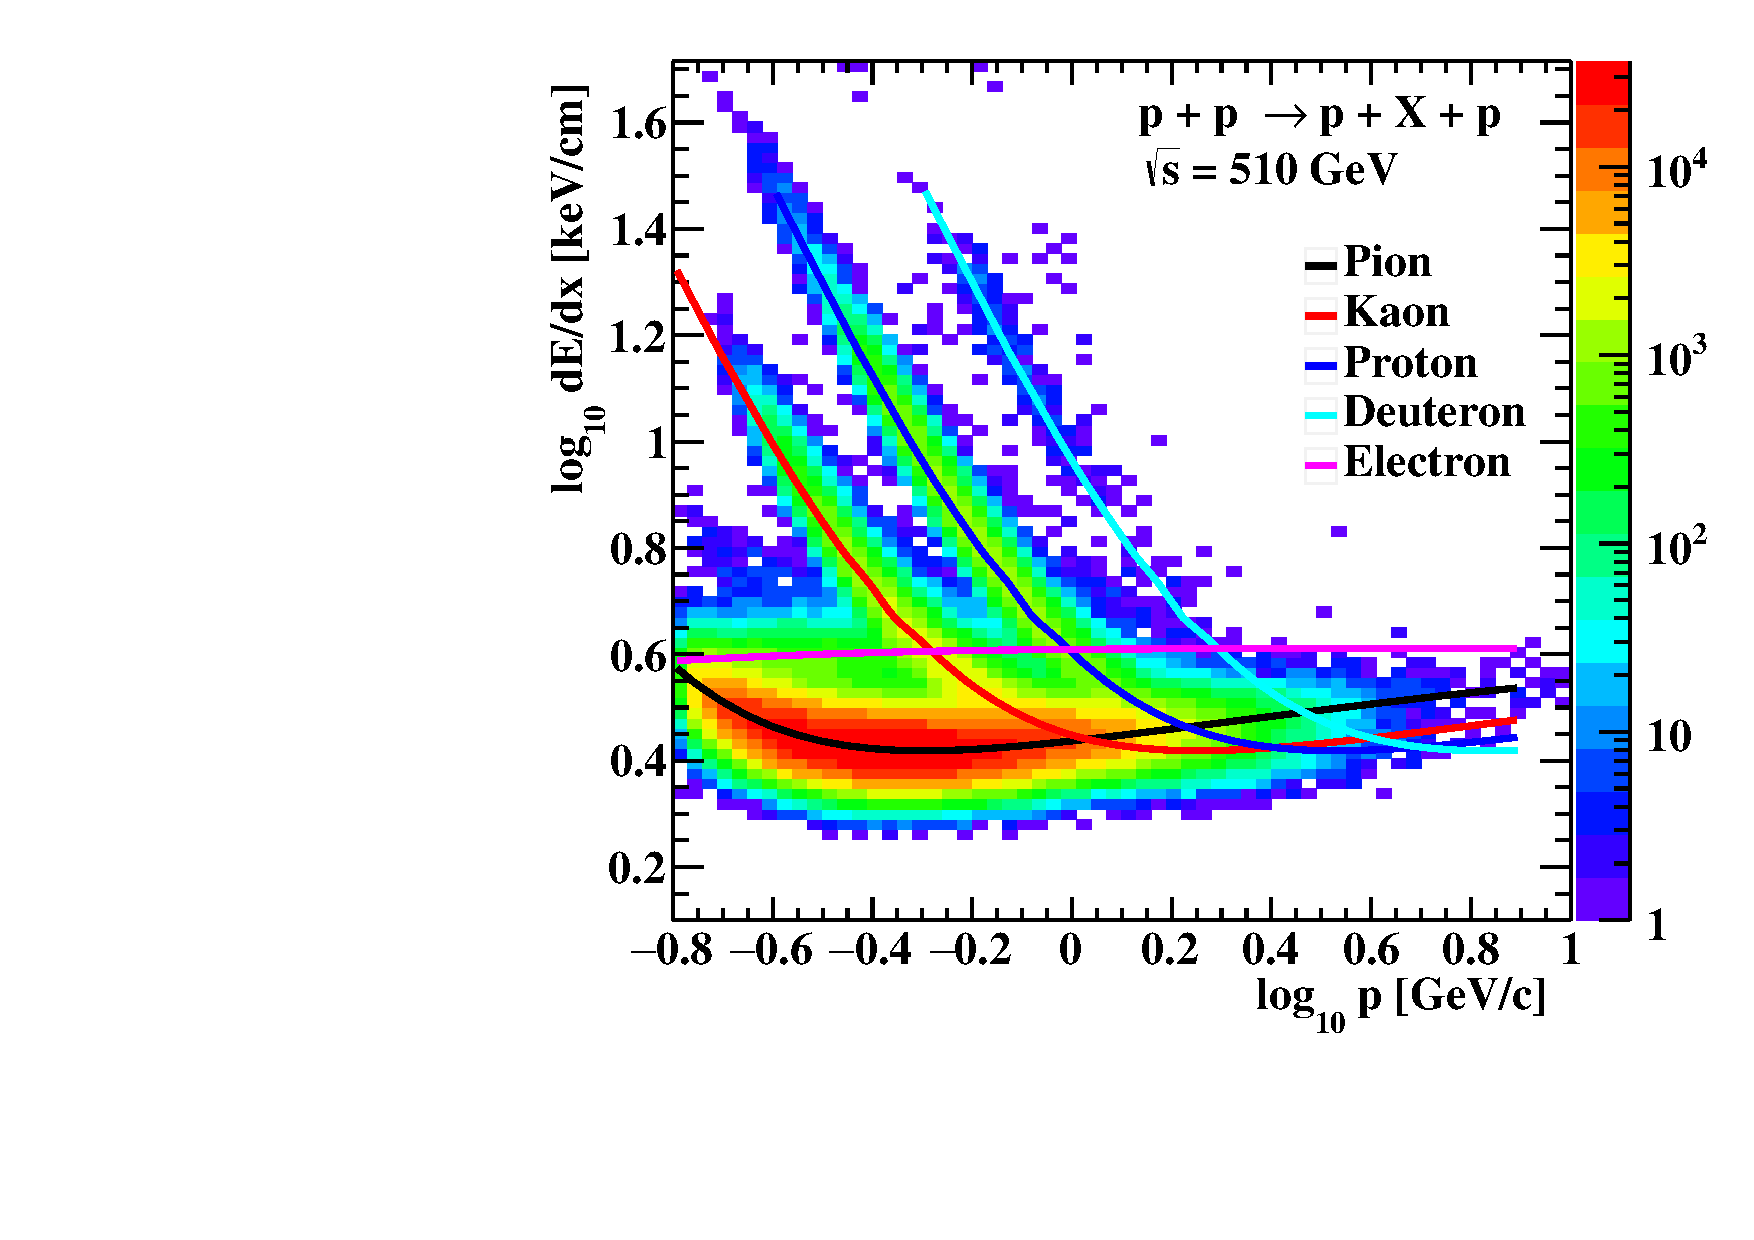
\includegraphics[width=1\textwidth]{figures/dEdx.pdf}
    \caption[Graph of hadron momentum and energy loss from TPC]{Correlation graph of hadron momentum and energy loss in keV/cm measured in TPC. All scales are logarithmic. }
    \label{af9}
\end{figure}
\FloatBarrier
\autoref{af9} shows that most of the particles that are measured by the TPC are pions, which are at the bottom of the graph and follow the black line. Next in line are kaons located around the red line followed by the protons positioned close to the blue line. The last line shown is the light blue line which represents deuterons. Even though the number of detected deuterons is negligible compared to number of other particles, there still are some. In \autoref{appendixA}, are shown the same graphs only they are divided based on the charge of particle. The graphs show that there are a few deuterons, but almost none antideuterons. Reason behind the detection of deuterons might be because of secondary interactions with particles in the beampipe.
\newline
The conditions for particle identification were as following,
\newline
\newline
\begin{minipage}{15cm}
\begin{myblock}{}
\centering
        $\textcolor{white}{\longrightarrow}if(n\sigma_{p}~<~3 ~~~\& ~~~n\sigma_{K}~>~3 ~~~\& ~~~n\sigma_{e}~>~3~~~ \& ~~~n\sigma_{\pi}~>~3)$
    \newline
    $\textcolor{white}{\longrightarrow}\textcolor{white}{\longrightarrow}$...
    \newline
        $\textcolor{white}{\longrightarrow}else~if(n\sigma_{p}~>~3 ~~~\& ~~~n\sigma_{K}~<~3 ~~~\& ~~~n\sigma_{e}~>~3~~~ \& ~~~n\sigma_{\pi}~>~3)$
    \newline
    $\textcolor{white}{\longrightarrow}\textcolor{white}{\longrightarrow}$...
    \newline
        $\textcolor{white}{\longrightarrow}else~if(n\sigma_{\pi}~<~3)$
    \newline
    $\textcolor{white}{\longrightarrow}\textcolor{white}{\longrightarrow}$...
\end{myblock}
\end{minipage}
\newline
\newline
First, protons were identified, on the grounds that the number of protons is the smallest (outside of deuterons which are irrelevant for this thesis). The condition imposed translates to particles being close enough to the proton line, but far enough from all the other lines. Same way were identified kaons. Lastly, pions are identified but they only have to satisfy the condition $n \sigma_{\pi}~<~3$. The reason for that is because pions are the majority of all particles and possible contamination with other particles is relatively low. Pions also hold a crucial role in the search for $K^0_S$ and $\Lambda^0$ and implementing a stronger condition might strongly affect the number of candidates for further analysis.
\FloatBarrier
\begin{figure}[ht]
    \centering
    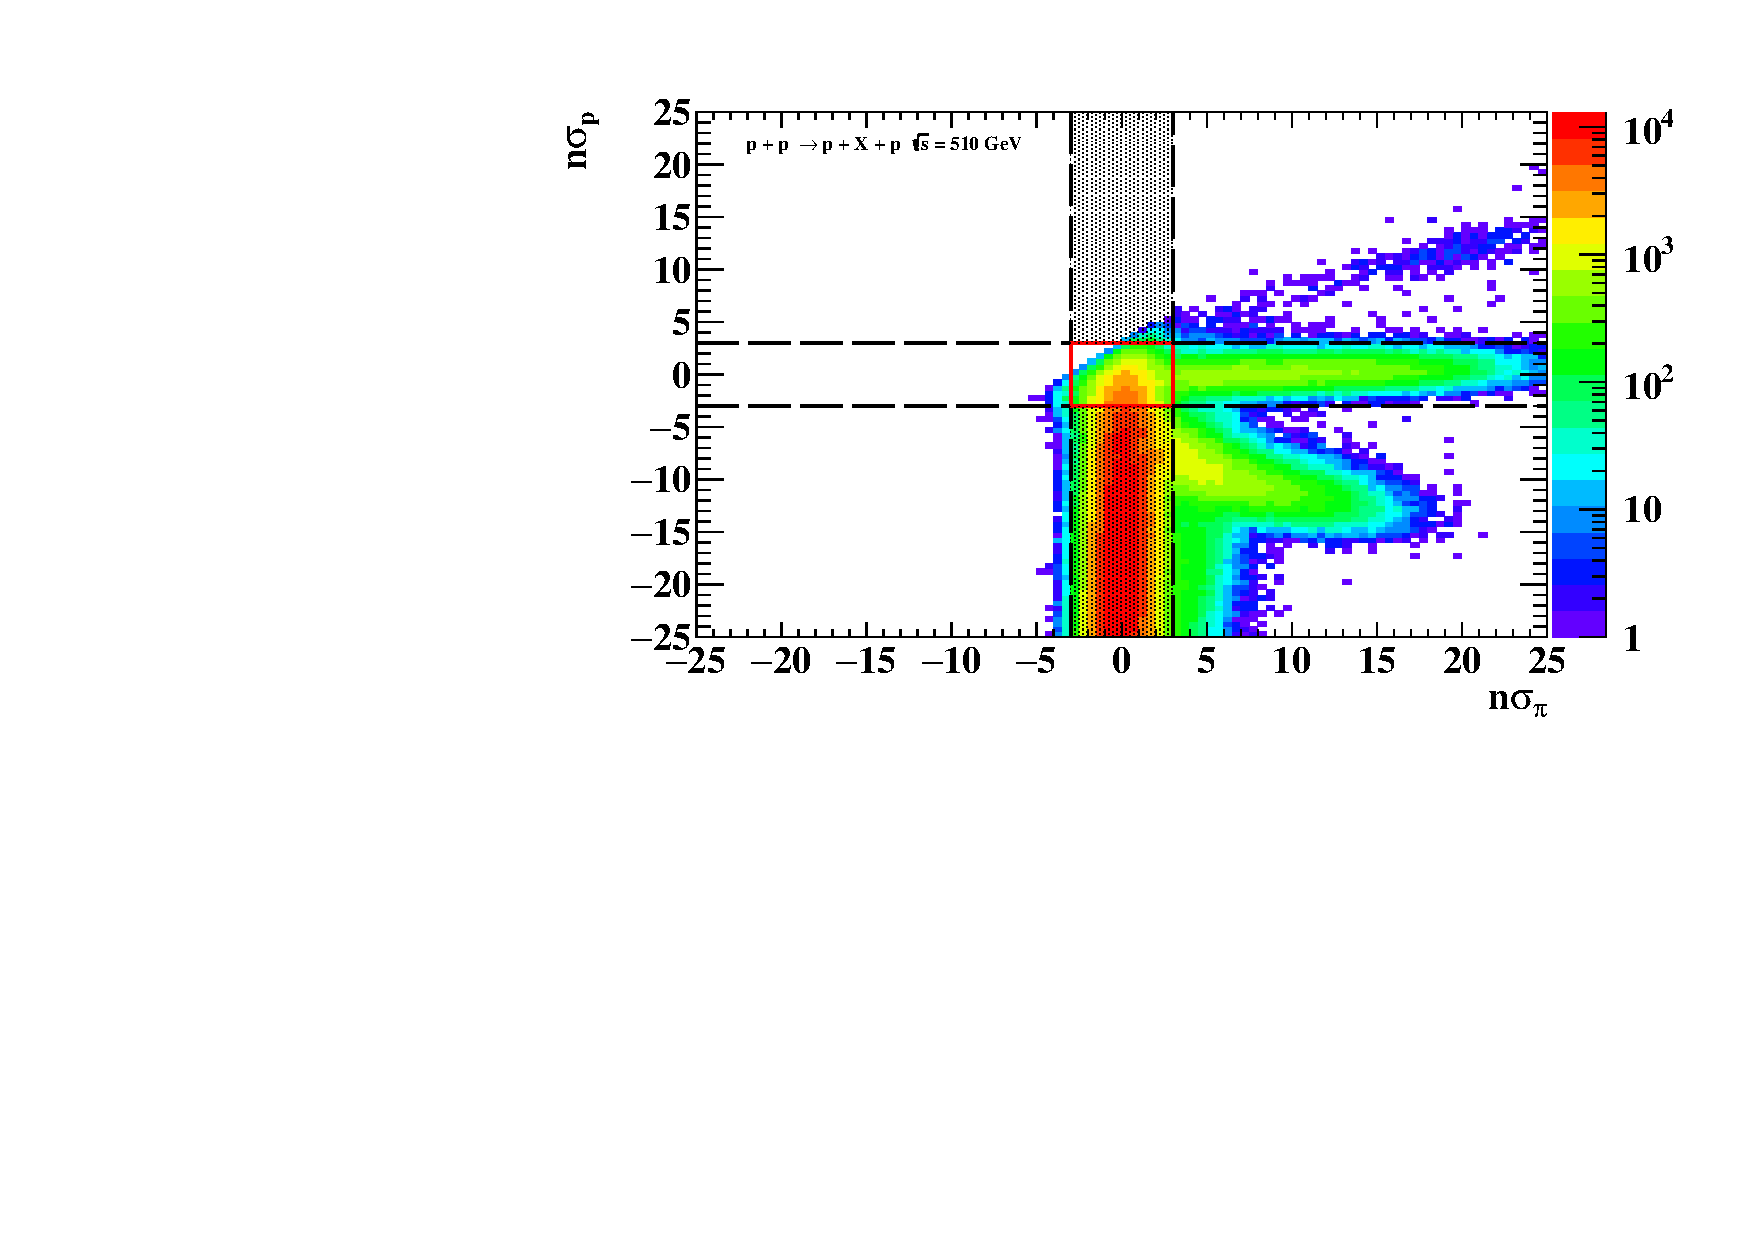
\includegraphics[width=1\textwidth]{figures/hNSigmaPiPcorr.pdf}
    \caption[Correlation graph of $n\sigma_{\pi}$ and $n\sigma_{p}$  of measured particles]{Correlation graph of $n_{\sigma}$ for pions on the x axis and $n_{\sigma}$ of protons on the y axis. Black lines represent the conditions for identification and the red box in the middle the overlay.}
    \label{af12}
\end{figure}
\FloatBarrier
\autoref{af12} is a correlation graph between $n \sigma$ for pions on the horizontal axis and protons on the vertical axis. Based on correlation plots for different particle pairs, which can be found in \autoref{appendixB}, particles on the right and parallel to pions in \autoref{af12} are electrons. Moving counter clockwise, the next band of particles represents kaons. Then follow protons and in last position are deuterons. 
 % Data Analysis
\newpage
\chapter{Results}
\label{resultS}
This chapter follows up the event selection and particle identification. All the conditions and cuts implemented in \autoref{analysis} helped sort through the massive number of events and pick the best candidates for further study. The focus of this chapter is on 2 particles: $K^0_S$ and $\Lambda^0$. Their peaks will be fitted with different distribution functions and results will be discussed. Part of search for $\Lambda^0$ are results for it's antiparticle $\overline{\Lambda}^0$. Differences between their production will be discussed. At the end of each section, exclusive production will be discussed. The analysis is still in progress and the results presented in this work have not yet been approved by the STAR collaboration for public presentation.
\section{Results for $K^0_S$}
\label{K0s}
Particle $K^0_S$ is one of two different neutral kaons, the other being $K^0_L$. The only difference between the two of them is their lifetime. The PDG value for lifetime of $K^0_S$ is $\tau_S = (8.954 \pm 0.004)10^{-11}$ s and for $K^0_L$ $\tau_L = (5.116 \pm 0.021)10^{-8}$ s. Kaons have spin 0 and parity -1. The dominant decay for $K^0_S$ is $\pi^+ \pi^-$. The other major decay is $\pi^0 \pi^0$. There are other, exotic decay channels, but their incidence is much less probable\cite{zyla}.
\newline
The invariant mass of identified charged pion pairs are shown in \autoref{af10}. Black histogram represents the unlike-sign pairs, red the like-sign pairs and green the difference. The green (and black) peak at around $500$ MeV is the $K^0_S$ peak. Following, at around $750-800$ MeV a wide peak can be seen. This peak could involve several other processes such as production of $\rho^0$ meson which decays in the 775 MeV channel. Following, at around 1000  and 1270 MeV are structures connected to exclusive production of pion pairs. They will be closely discussed at the end of this section.
\FloatBarrier
\begin{figure}[ht]
    \centering
    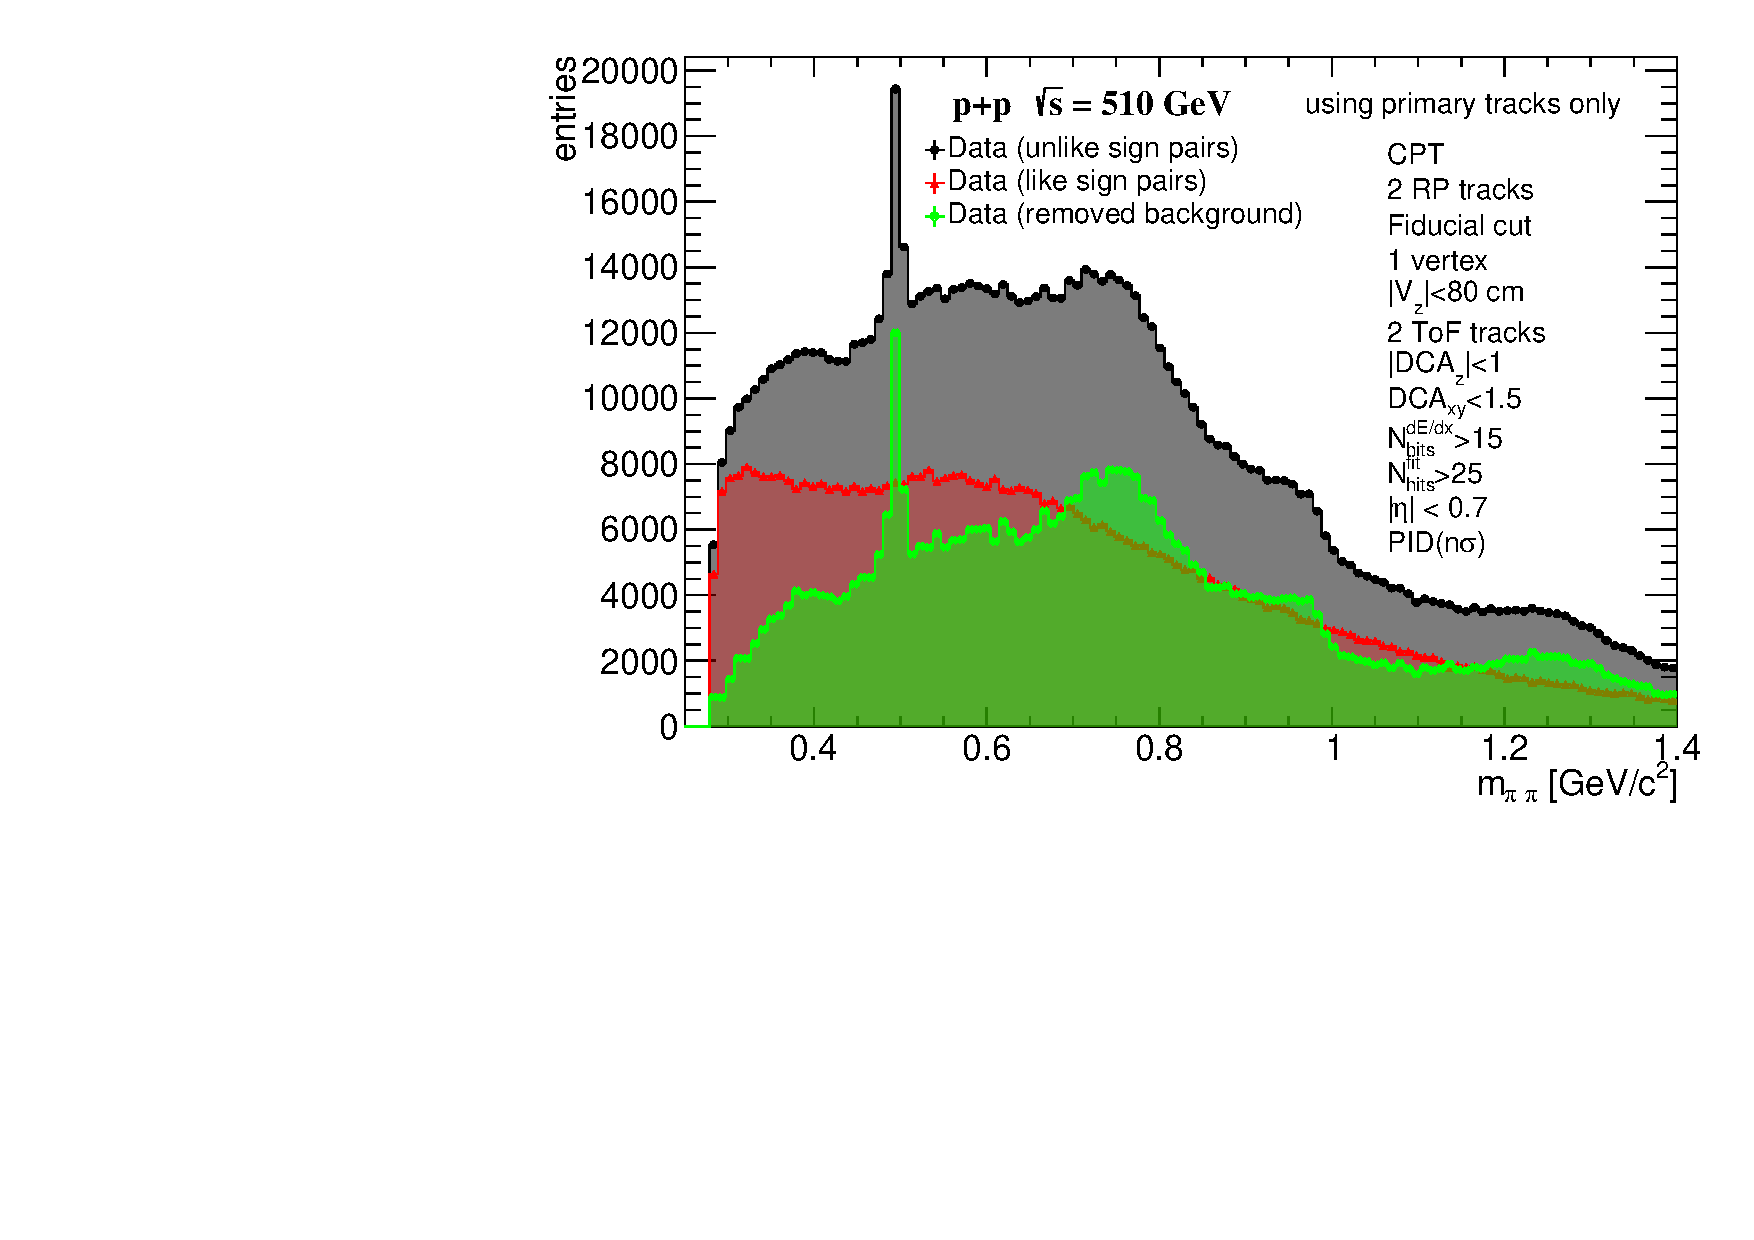
\includegraphics[width=1\textwidth]{figures/invMassLikeUnlikeK0s.pdf}
    \caption[Distribution of invariant mass of $\pi^+ \pi^-$ pairs]{Distribution of invariant mass of identified $\pi^+ \pi^-$ pairs. Black represent the unlike-sign pairs, red the like-sign pairs and green the difference.}
    \label{af10}
\end{figure}
\FloatBarrier
The peak for $K^0_S$ in like-sign pairs was first fitted with Gauss distribution and 1. degree polynomial and later with Gauss distribution and 2. degree polynomial. Functions of both fits are shown as \autoref{er1} and \autoref{er2} respectively. Fits can be seen in \autoref{af11} and \autoref{af13}. Green line represents the fit and red is the polynomial which serves as background. Parameters for red polynomial are the same as for the green fit. 
\newline
\begin{equation}
\centering
f_1(x) = p_0x + p_1x + Ae^{-\frac{(x-\mu)^2}{2\sigma^2}}
\label{er1}
\end{equation}
\begin{equation}
\centering
f_2(x) = p_0x + p_1x + p_2x^2 + Ae^{-\frac{(x-\mu)^2}{2\sigma^2}}
\label{er2}
\end{equation}
The quality of fit is evaluated using the ratio $\frac{\chi^2}{ndf}$. Value $\chi^2$ is the sum of quadratic deviations of fit from the data points. Value $ndf$ stands for number of degrees of freedom\footnote{Value for $ndf$ is calculated as the difference between the number of fitted data points and number of parameters of the fit.}. A good quality fit should have ratio close to 1. Yield was also calculated using the following equation,
\begin{equation}
\centering
y = \frac{1}{norm}(\int^{b}_{a}f_g(x)\mathrm{d}x - \int^{b}_{a}f_r(x)\mathrm{d}x)
\label{er6}
\end{equation}
where $norm$ is a normalization factor and is the size of 1 bin in GeV. Upper and lower  limits of integrals, $a$ and $b$, use values from fit and can be computated as $b=\mu + 3\sigma$ and $a=\mu - 3\sigma$. Results of fit 1 and fit 2, qualities of fits and yields are in \autoref{at1}. 
\FloatBarrier
\begin{figure}[ht]
    \centering
    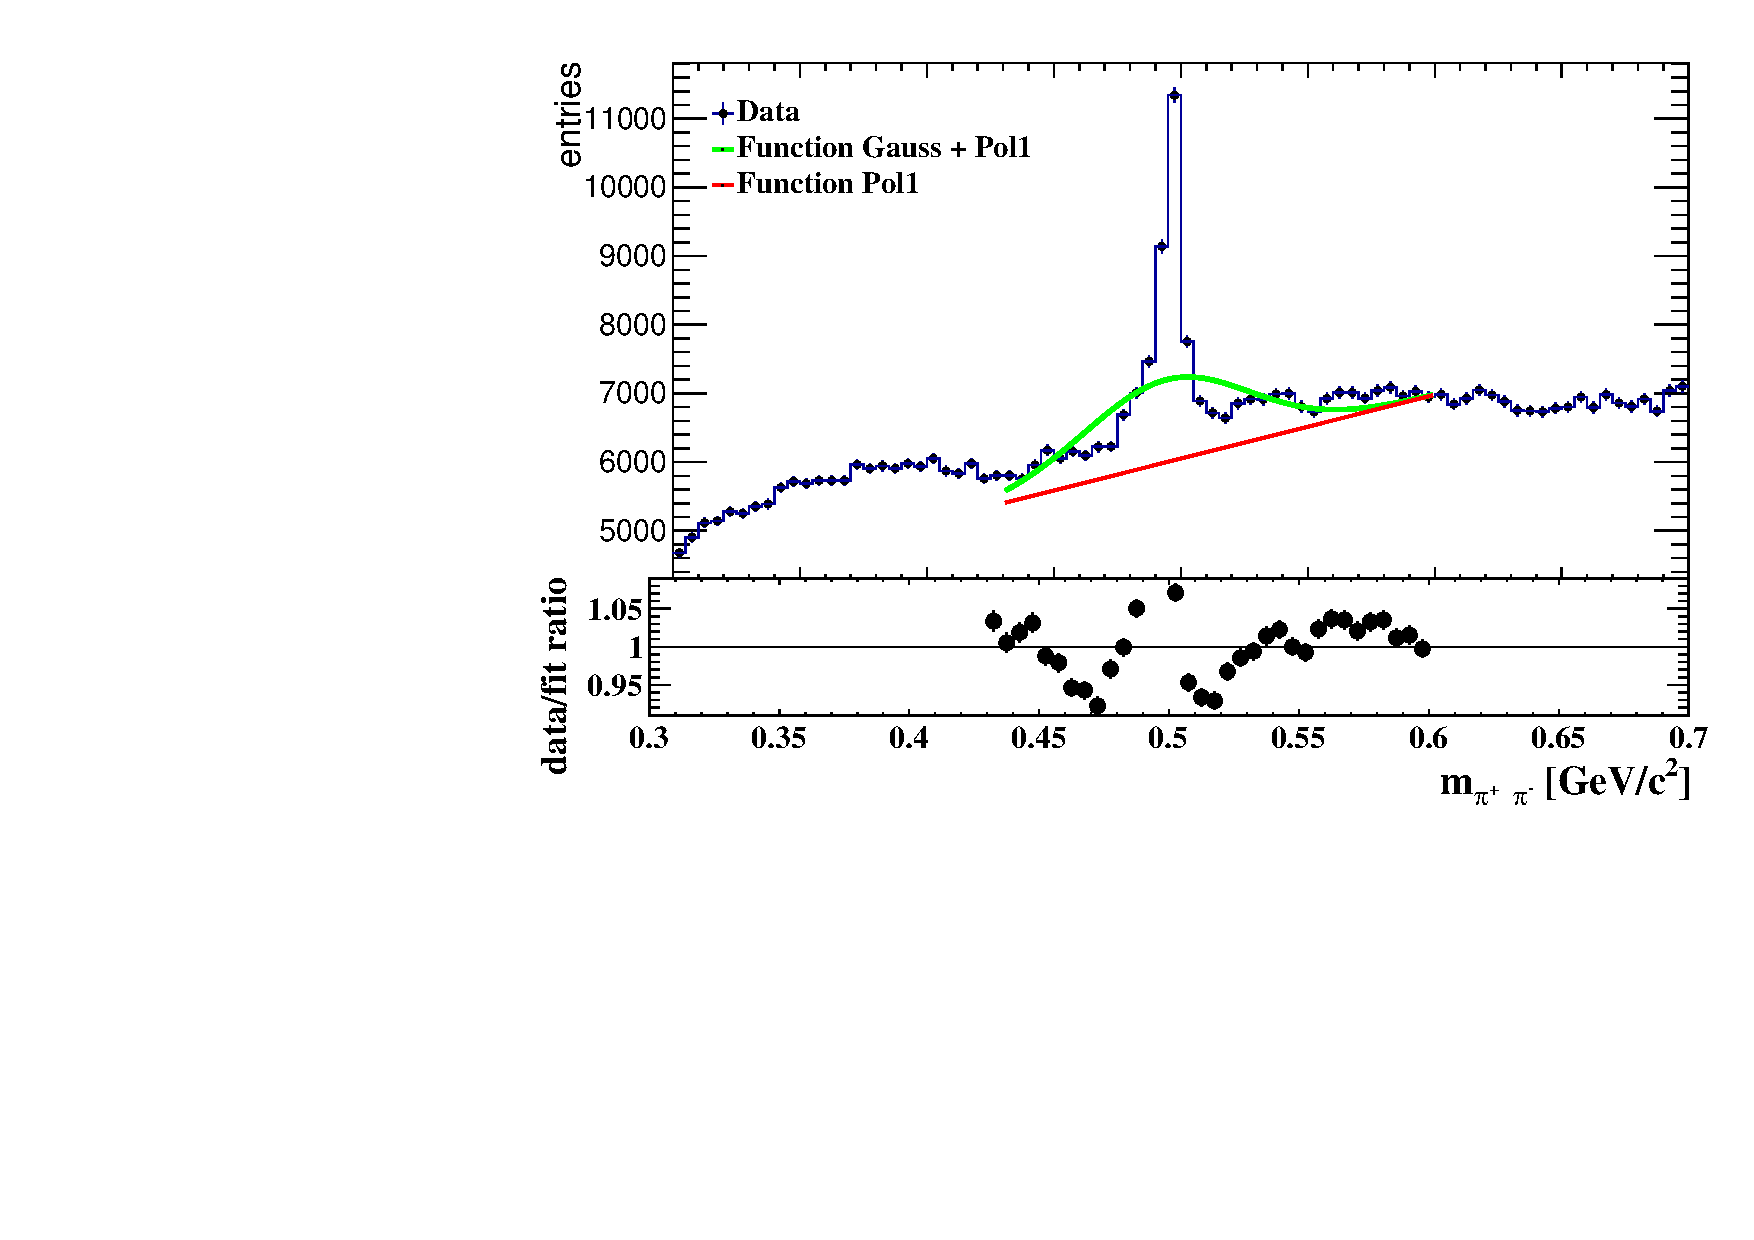
\includegraphics[width=1\textwidth]{figures/K0sFitLinear.pdf}
    \caption[Distribution of invariant pion pairs fitted with Gauss distribution and 1. degree polynomial]{Distribution of invariant mass of $\pi^+ \pi^-$ pairs fitted with a a Gauss distribution function and a first degree polynomial \autoref{er1}. Results of fit are in \autoref{at1}.}
    \label{af11}
\end{figure}
\FloatBarrier

\FloatBarrier
\begin{table}[ht]
    \centering
        \begin{tabular}{c|c|c}
             & Fit 1 & Fit 2 \\ \hline
           $p_0$ & $4.6 \pm 0.2$(stat) $10^{3}$ & $-2.1 \pm 0.3$(stat) $10^{4}$ \\ \hline
           $p_1$ & $1.15 \pm 0.04$(stat) $10^4$ & $1.1 \pm 0.1$(stat) $10^5$\\ \hline
           $p_2$ & & $-1 \pm 1$(stat) $10^4$ \\ \hline
           $A$ & $6.8 \pm 0.1$(stat) $10^3$ &  $6.6 \pm 0.1$(stat) $10^3$ \\ \hline
           $\mu$ & $0.4956 \pm 0.0001$(stat) &  $0.4955 \pm 0.0001$(stat) \\ \hline
           $\sigma$ & $4.79 \pm 0.09$(stat) $10^{-3}$ &  $4.6 \pm 0.1$(stat) $10^{-3}$ \\ \hline
           $a$ & $0.4812$ & $0.4819$\\ \hline
           $b$ & $0.5010$ & $0.5092$ \\ \hline
           $norm$ & $0.008$ & $0.008$ \\ \hline
           $\chi^2$ & $145$ & $57$ \\ \hline
           $ndf$ & $17$  & $16$ \\ \hline
           $\frac{\chi^2}{ndf}$ & $8.5$ & $3.6$  \\ \hline
           $y$ & $10~200 \pm 500$(stat) & $9~400 \pm 300$(stat)
        \end{tabular}
    \caption[Results for fit 1 and 2 of invariant mass of $\pi^+ \pi^-$ pairs]{Results for fit 1 and 2 of peak for $\pi^+ \pi^-$ invariant mass distribution, qualities of fit and yields. Description of variables and the fit functions are in text.}
    \label{at1}
\end{table}
\FloatBarrier
\FloatBarrier
\begin{figure}[ht]
    \centering
        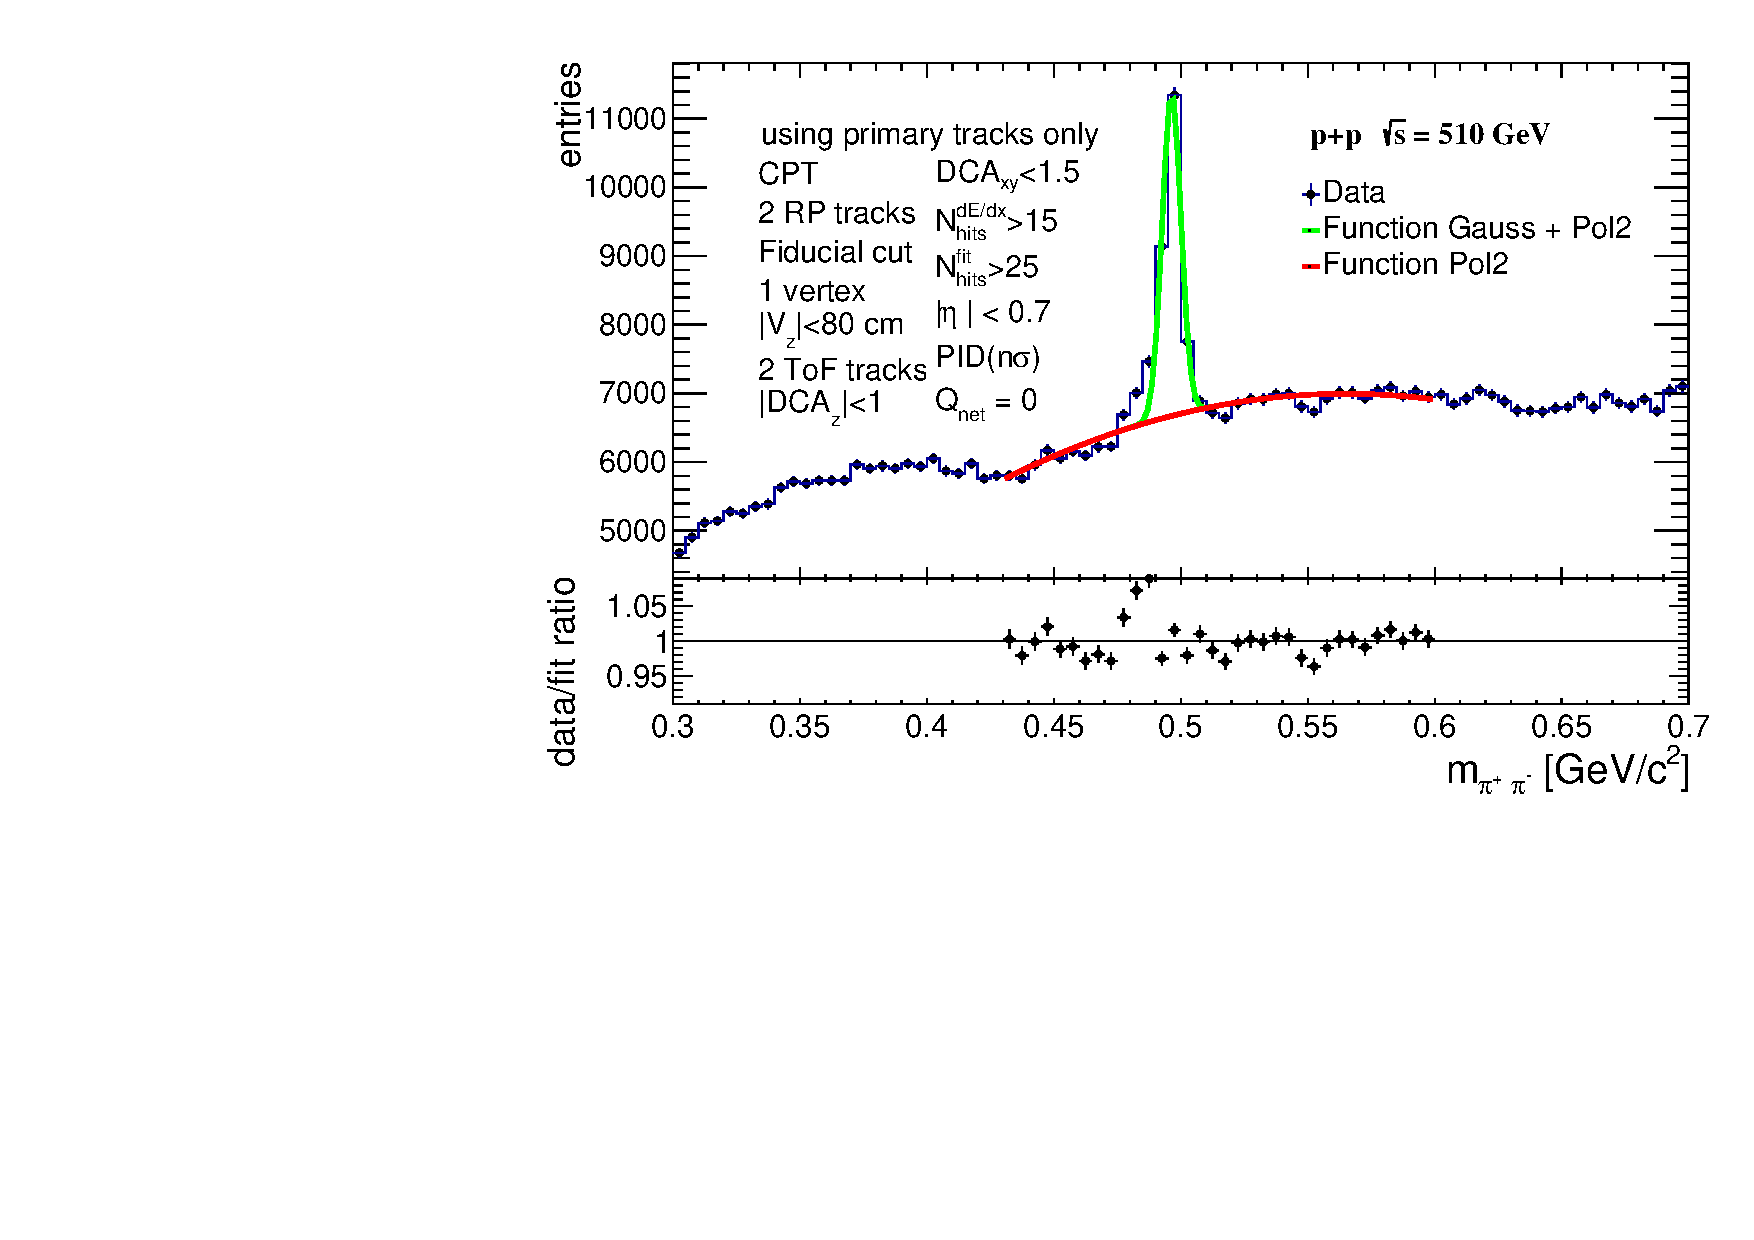
\includegraphics[width=1\textwidth]{figures/K0sFitQuad.pdf}
        \caption[Distribution of invariant pion pairs fitted with Gauss distribution and 2. degree polynomial]{Distribution of invariant mass of $\pi^+ \pi^-$ pairs. Fitted with function of Gauss distribution and second degree polynomial.}
    \label{af13}
\end{figure}
\FloatBarrier
%\FloatBarrier
%\begin{table}[ht]
    %\centering
        %\begin{tabular}{c|c}
           %$p_0$ & $-2.1 \pm 0.3$(stat) $10^{4}$\\ \hline
           %$p_1$ & $1.1 \pm 0.1$(stat) $10^5$ \\ \hline
           %$p_2$ & $-1 \pm 1$(stat) $10^4$ \\ \hline
           %$A$ & $6.6 \pm 0.1$(stat) $10^3$ \\ \hline
           %$\mu$ & $0.4955 \pm 0.0001$(stat) \\ \hline
           %$\sigma$ & $4.6 \pm 0.1$(stat) $10^{-3}$ \\ \hline
           %$a$ & $0.4819$ \\ \hline
           %$b$ & $0.5092$ \\ \hline
           %$norm$ & $0.008$ \\ \hline
           %$\chi^2$ & $57$ \\ \hline
           %$ndf$ & $16$  \\ \hline
           %$\frac{\chi^2}{ndf}$ & $3.6$ \\ \hline
           %$y$ & $9~400 \pm 300$(stat)
        %\end{tabular}
    %\caption[Results for fit 2 of invariant mass of $\pi^+ \pi^-$ pairs]{Results of fitted peak for $\pi^+ %\pi^-$ invariant mass distribution, quality of fit and yield. Fit function is shown in \autoref{er2}.}
    %\label{at2}
%\end{table}
%\FloatBarrier
The expected value, $\mu$, which was fitted as parameter in both fits, represents the decay channel of $K^0_S$ and it's invariant mass. Values from both fits correspond to official PDG value of invariant mass of $K^0$: $497.611$  $\pm$ 0.013 MeV. 
\newline
To take a closer look at exclusive production of $K^0_S$, the missing transverse momentum was computed\footnote{Momenta of 4 measured particles (2 forward protons and 2 central pions) in $(x,y)$ directions were summed.}. Exclusive production would mean the missing transverse momentum would within 0. Distribution of missing transverse momentum is shown in \autoref{af49} with a cut at 100 MeV. The distribution of invariant mass of candidates that passed this condition is shown in \autoref{af50}.

\FloatBarrier
\begin{figure}[ht]
    \centering
    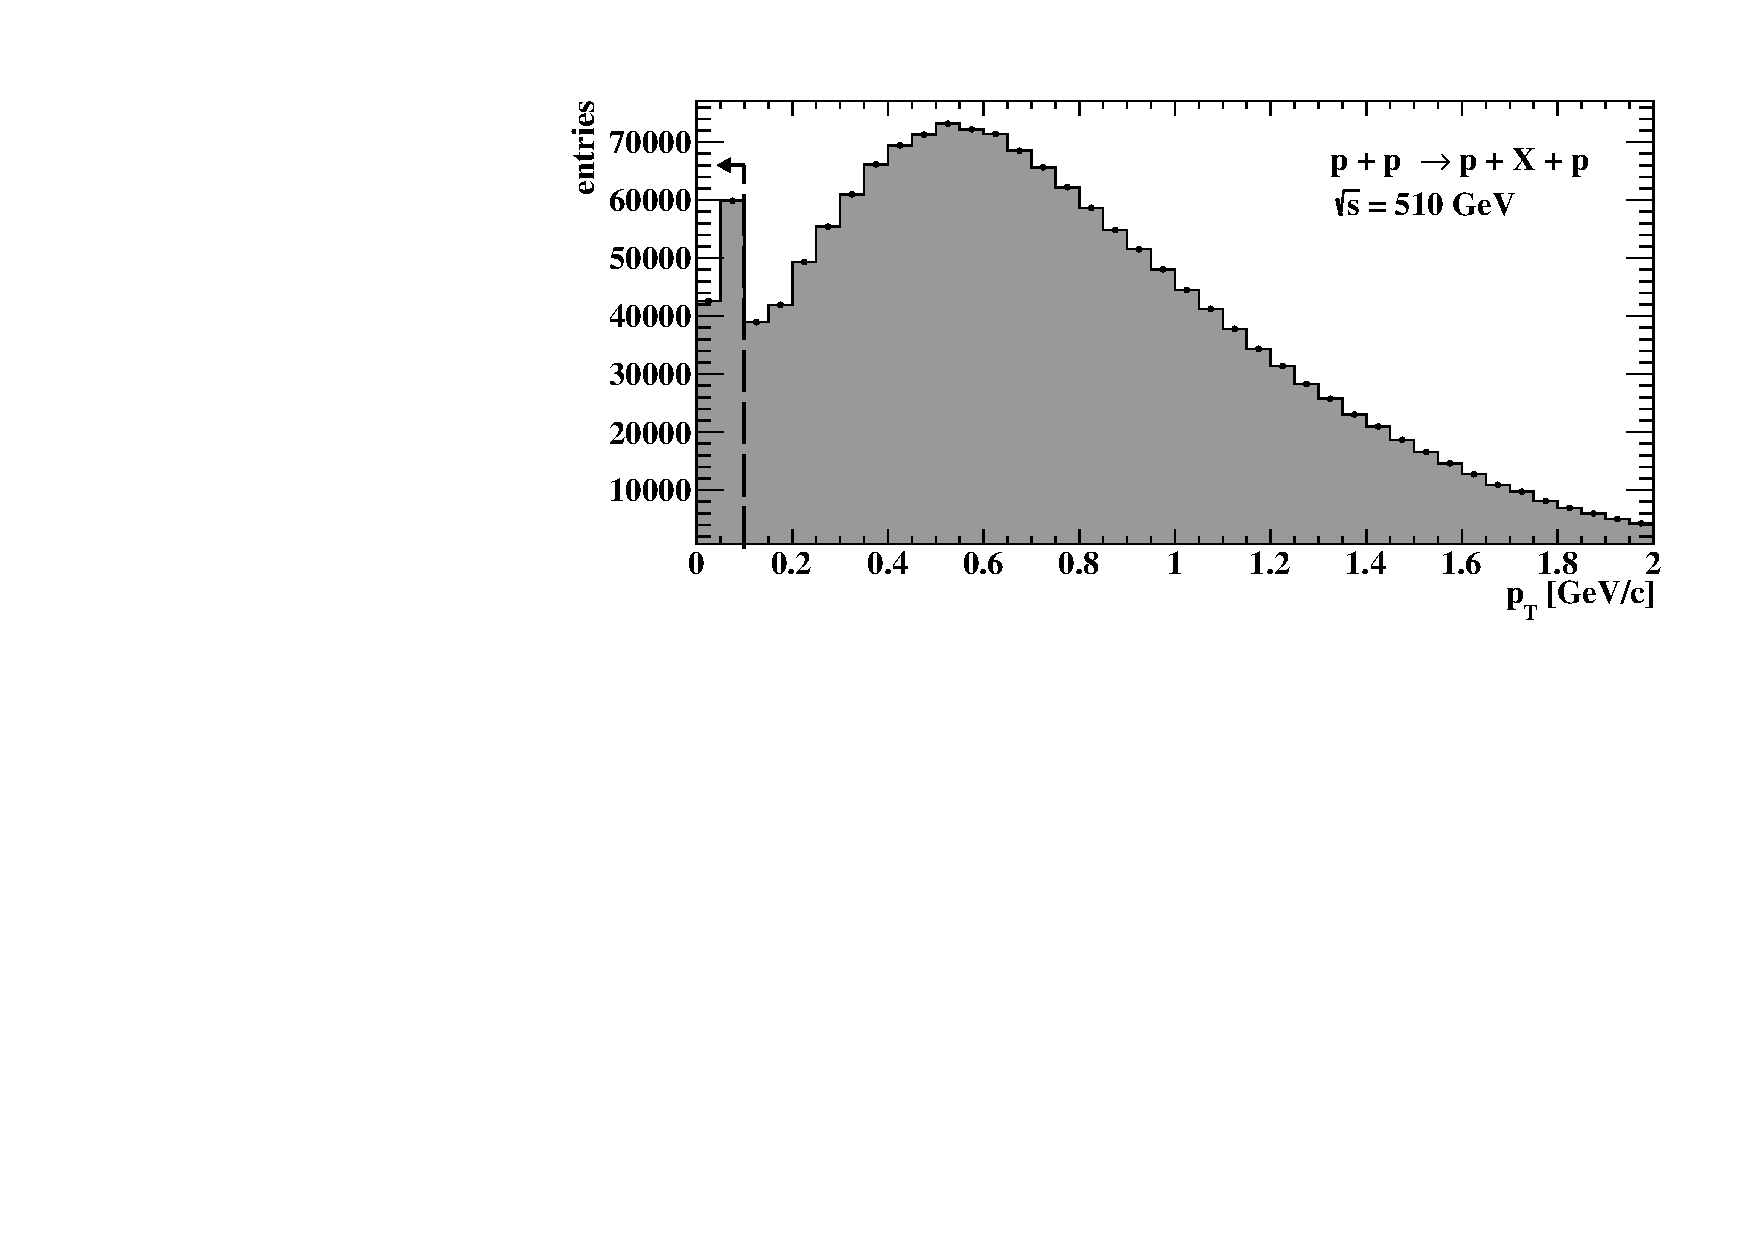
\includegraphics[width=1\textwidth]{figures/hPtMissingK0s.pdf}
    \caption[Distribution of missing transverse momentum for $\pi \pi$ pairs]{Distribution of missing transverse momentum for particle $\pi^+ \pi^-$ pairs. Arrow represents a cut at 100 MeV.}
    \label{af49}
\end{figure}
\FloatBarrier

\FloatBarrier
\begin{figure}[ht]
    \centering
    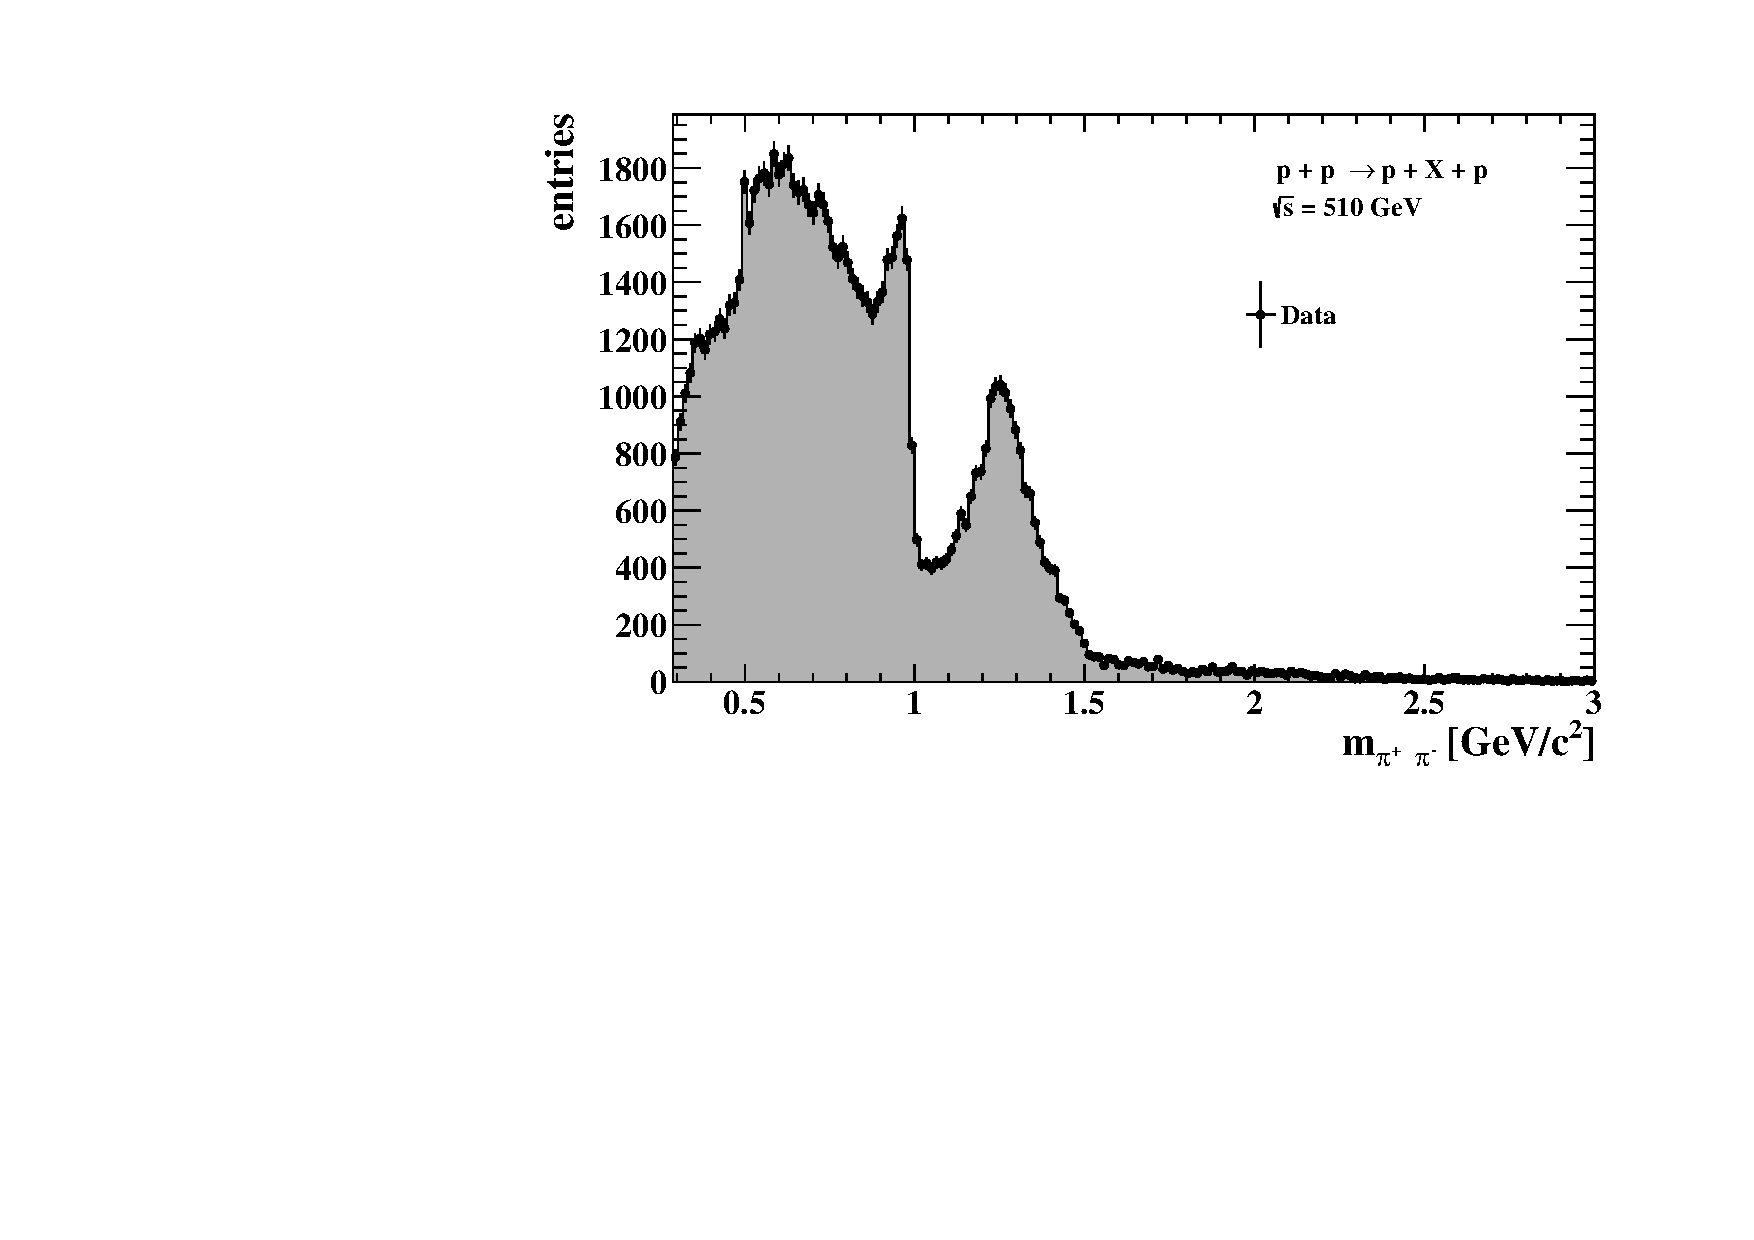
\includegraphics[width=1\textwidth]{figures/invMassPiPiexclusive.pdf}
    \caption[Distribution of invariant mass of exclusively produced $\pi \pi$ pairs]{Distribution of invariant mass of $\pi \pi$ pairs that were created with exclusive production. Black points represent unlike-sign pairs and red like-sign.}
    \label{af50}
\end{figure}
\FloatBarrier

Distribution shown in \autoref{af50} has many similarities to distributions discussed in \autoref{theoretics}, \autoref{recent}. They were visible even without the condition for exclusive production in \autoref{af10}, but the structures here are much more significant. Even though it is within the uncertainties, a slight peak at around 500 MeV can be seen which could represent $K^0_S$. If it was more significant, it could mean some level of contamination of data. Distribution then rises and later decreases. Sharp peak right before 1 GeV which corresponds to resonance $f_0$(980) followed by a very steep drop. Resonance $f_2$(1270) at 1270 MeV can also be seen as a tall and wide peak. All of these correspond to results discussed in \autoref{theoretics}, \autoref{recent}. 

\section{Results for $\Lambda^0$}
\label{Lambda}
Particle $\Lambda^0$ and it's antiparticle $\overline{\Lambda}^0$ are neutral baryons\footnote{Baryons are particles composed out of 3 quarks.} which mostly decay to $p \pi^-$ and $\overline{p} \pi^+$ respectively\footnote{Decay $\Lambda^0 \longrightarrow \overline{p} \pi^+$ is forbidden because it does not satisfy the law of conservation of baryon number.}. Second most probable decay for $\Lambda^0$ is into pair $\pi^0 n$.


\FloatBarrier
\begin{figure}[ht]
    \centering
    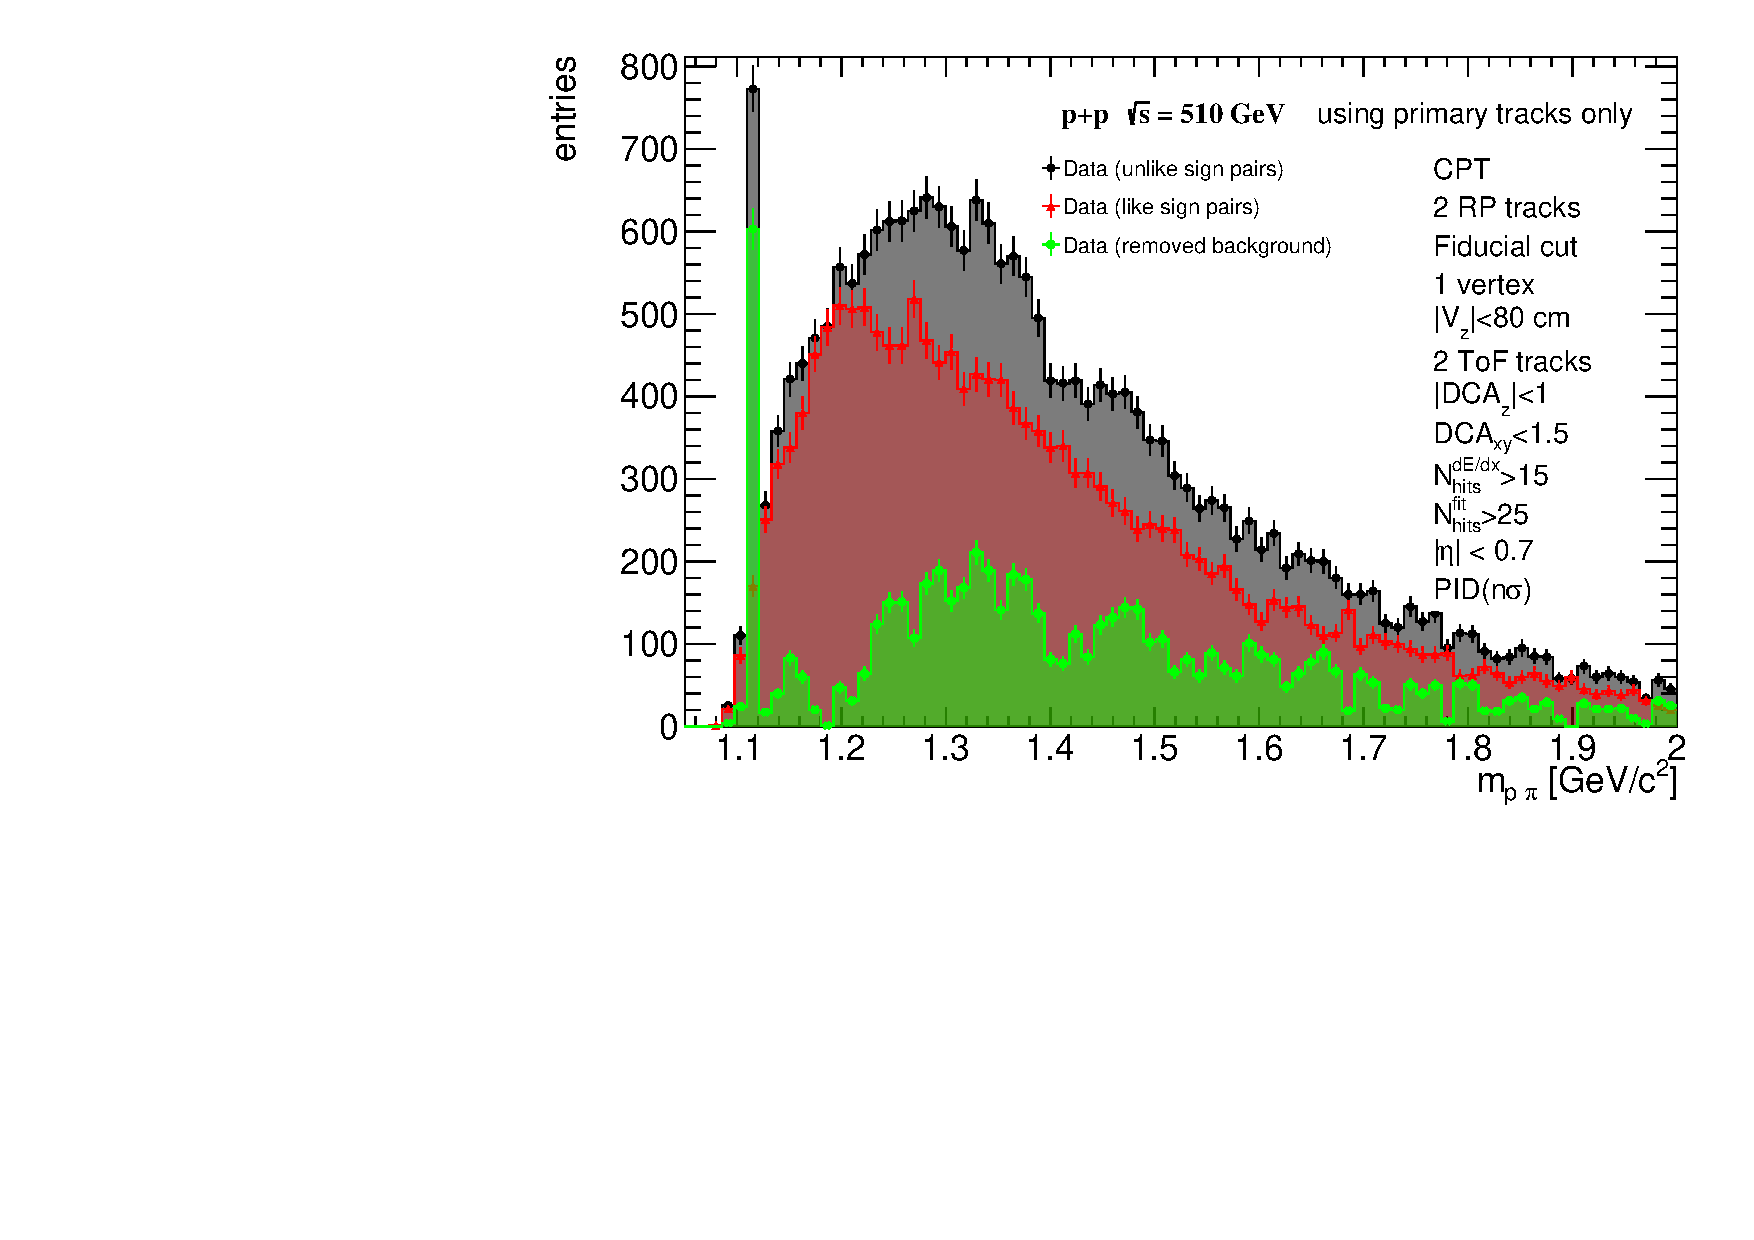
\includegraphics[width=1\textwidth]{figures/invMassLikeUnlikeLambda.pdf}
    \caption[Results for fit 1 of invariant mass of $p \pi$ pairs]{The distribution of invariant mass for identified $p \pi$ pairs.  Black represent the unlike-sign pairs, red the like-sign pairs and green the difference.}
    \label{af14}
\end{figure}
\FloatBarrier
Invariant mass distributions of $p \pi$ pairs are shown in \autoref{af14}. Black represents unlike-sign pairs, red like-sign pairs and green is the difference. Peak at around $1.1$ GeV is the $\Lambda^0$ or $\overline{\Lambda}^0$. The statistics for this distribution is much smaller than for $K^0_S$ and the background is of similar scale to unlike-sign pairs. Therefore, the green signal, aside from $\Lambda$ peak, is quite small. Only possible structure is a slight dip at around $1.4$ GeV. Otherwise, like- and unlike-sign pair distributions have very similar shapes. 
\FloatBarrier
\begin{figure}[ht]
    \centering
    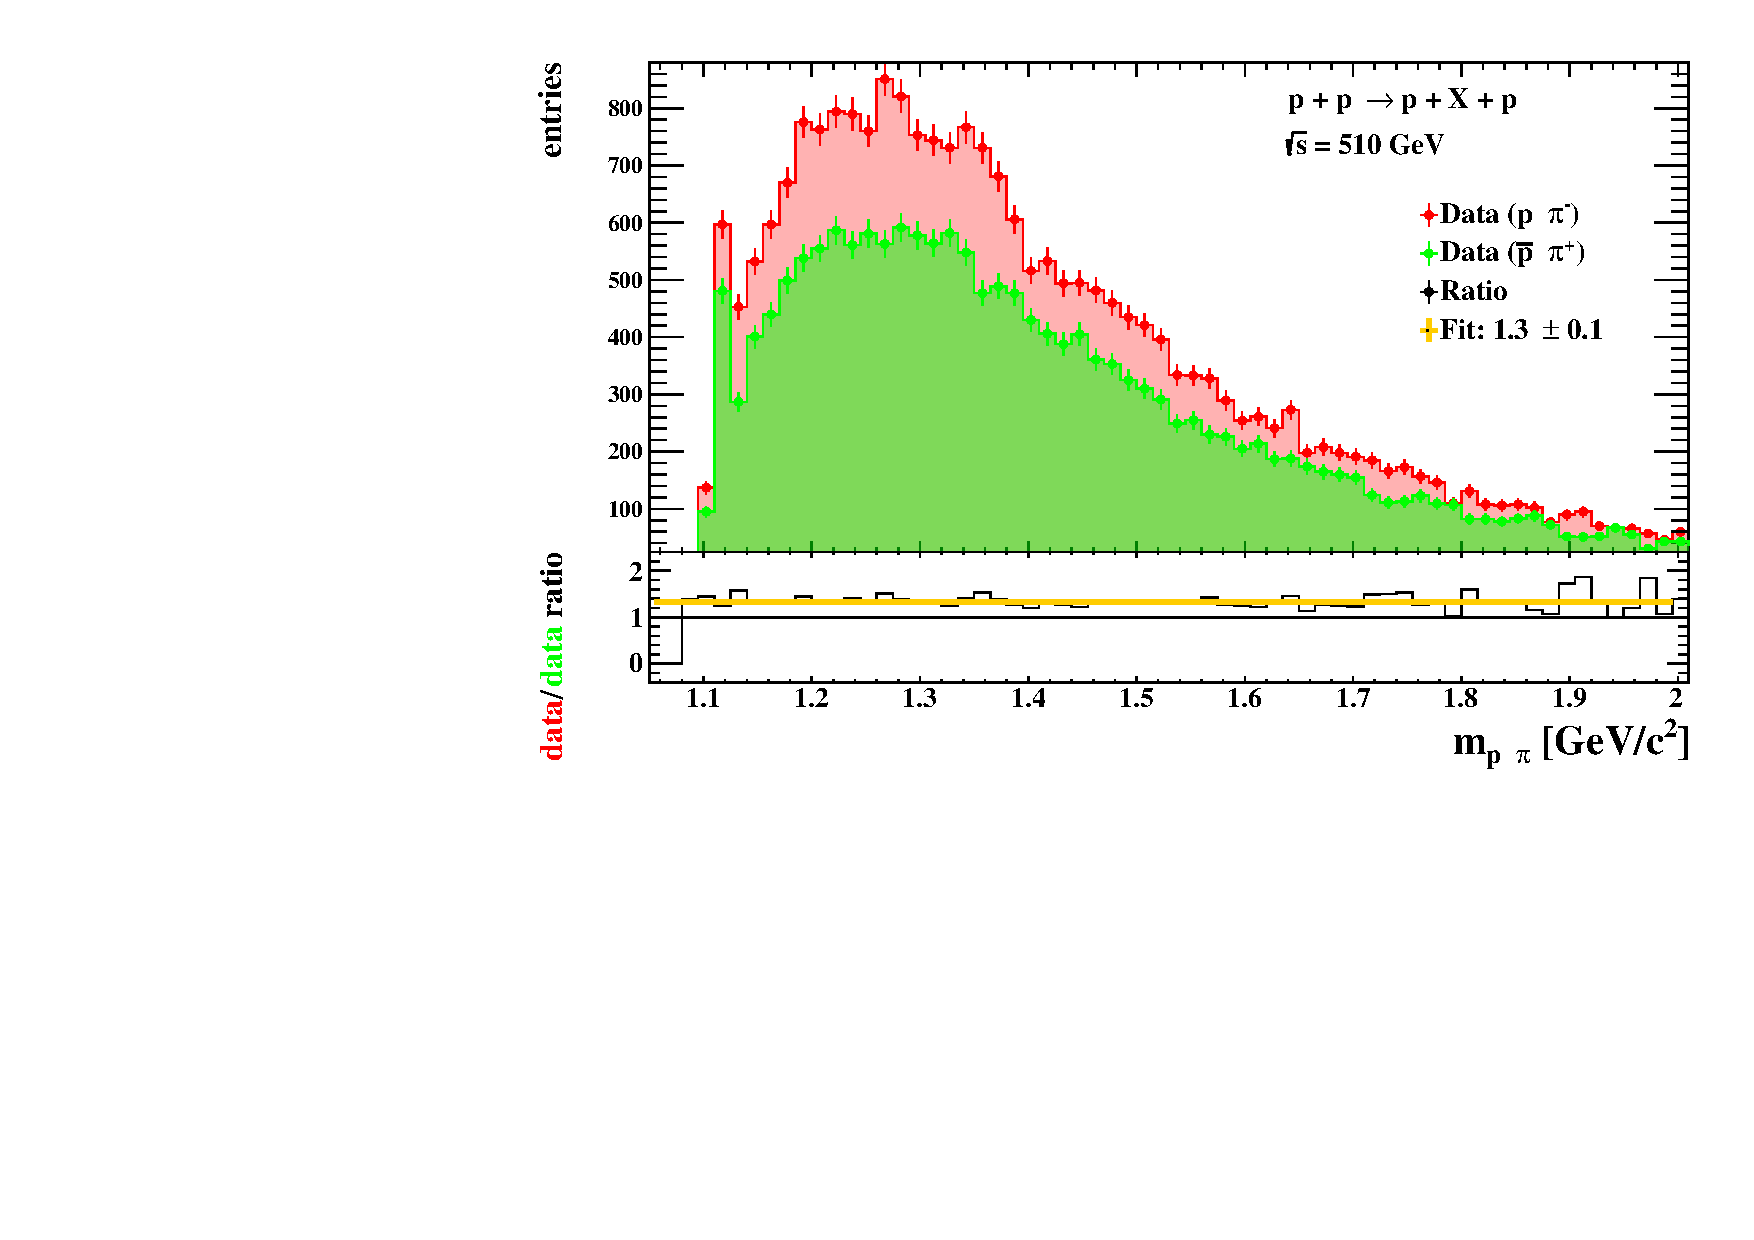
\includegraphics[width=1\textwidth]{figures/LambdaAntiLambda.pdf}
    \caption[Distributions of invariant mass for $p \pi^-$ and $\overline{p} \pi^+$ pairs]{Distributions of invariant mass for $p \pi^-$ (green) and $\overline{p} \pi^+$ (red) pairs. Underneath is a ratio plot which is fitted with a constant function.}
    \label{af19}
\end{figure}
\FloatBarrier

\FloatBarrier
\begin{figure}[ht]
    \centering
    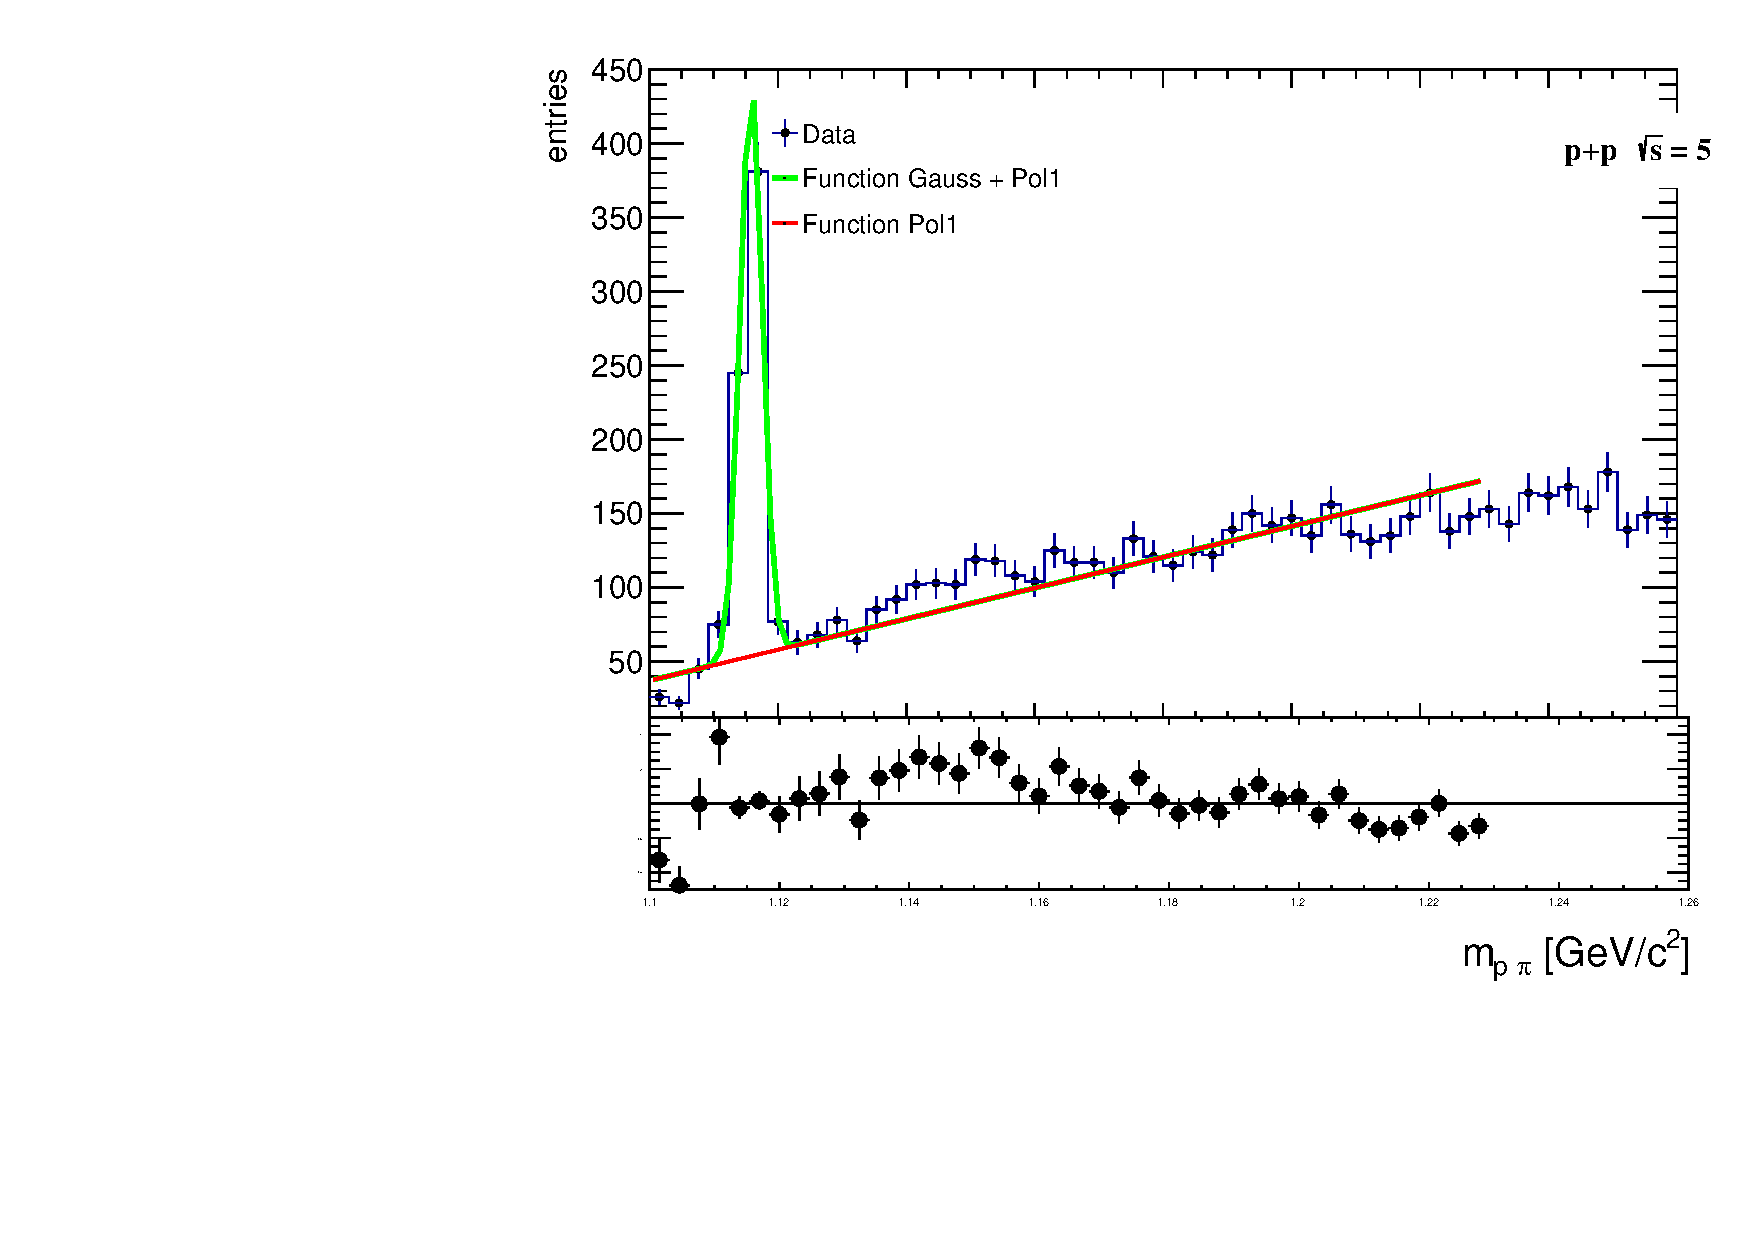
\includegraphics[width=1\textwidth]{figures/LambdaFitLinear.pdf}
    \caption[Distribution of invariant pion proton pairs fitted with Gauss distribution and 1. degree polynomial]{The distribution of invariant mass for identified $p$ $\pi$ pairs fitted with Gauss distribution function and first degree polynomial. Results of fit can be found in \autoref{at3}.}
    \label{af15}
\end{figure}
\FloatBarrier
\autoref{af19} shows the difference between $p \pi^-$ and $\overline{p} \pi^+$ distributions. Shapes of the distributions are very similar- both follow the distributions shown in \autoref{af14} which is the expected shape. The only noticeable difference is the scaling of both structures. Ratio of measured data is underneath and is fitted with a constant function. The result of fit: $1.3 \pm 0.1$. This could possibly be because of lower efficiency in measuring antimatter.
\newline
Peaks from unlike-sign distributions of invariant mass for $p \pi$ pairs were fitted similarly to fits for $K^0_S$. First fit was Gauss distribution and 1. degree polynomial shown in \autoref{er1}. Second fit was again, Gauss distribution and 2. degree polynomial and can be found in \autoref{af16}. Results of both fits can be found in \autoref{at3}. The qualities of fits were calculated the same way as for $K^0_S$. 
\FloatBarrier
\begin{table}[ht]
        \centering
        \begin{tabular}{c|c|c}
             & Fit 1 & Fit 2 \\ \hline
           $p_0$ & $-1.02 \pm 0.04$(stat) $10^{3}$ & $-1.105$ $ \pm$ $ 0.0002$(stat) $10^{4}$ \\ \hline
           $p_1$ & $9.6 \pm 0.04$(stat) $10^2$ &  $1.829$ $ \pm$ $ 0.0002$(stat) $10^4$  \\ \hline
           $p_2$ & $-7.48$ $ \pm$ $ 0.01$(stat) $10^3$ \\ \hline
           $A$ & $3.6 \pm 0.2$(stat) $10^2$ & $3.6$ $ \pm$ $ 0.2$(stat) $10^3$ \\ \hline
           $\mu$ & $1.11569$ $ \pm$ $ 0.00009$(stat) & $1.11567$ $\pm$ $ 0.00007$(stat)  \\ \hline
           $\sigma$ & $1.70$ $ \pm$ $ 0.07$(stat) $10^{-3}$ &  $1.71$ $ \pm$ $ 0.07$(stat) $10^{-3}$\\ \hline
           $a$ & $1.1106$ & $1.1105$\\ \hline
           $b$ & $1.1208$ &$1.1208$ \\ \hline
           $\chi^2$ & $94$ & $41$\\ \hline
           $ndf$ & $41$  &  $37$\\ \hline
           $\frac{\chi^2}{ndf}$ & $2.3$ & $1.1$ \\ \hline
           $y$ & $540 \pm 50$(stat) & $540 \pm 50$(stat)
        \end{tabular}
    \caption[Results for fit 1 and 2 of invariant mass of $p \pi$ pairs.]{Results of fits for peak of $p ~\pi^- $ and $\overline{p}~\pi^+$ invariant mass distribution, quality of fit and yield. Description of variables is in text. }
    \label{at3}
\end{table}
\FloatBarrier
Gauss distribution follows the peak in both fits very well. The quality test $\frac{\chi^2}{ndf}$ of both fits is better compared to $K^0_S$ fits. Especially the second fit for $\Lambda$. When it comes to modeling the shape of the background, 2. degree polynomial is superior to 1. degree polynomial. The expected values for both fits, $\mu$, correspond to PDG value for invariant mass of particle $\Lambda^0$: $1115.683$ $\pm$ $0.006$ MeV \cite{zyla}.
\newline
Missing transverse momentum for $p \pi$ pairs is drawn in \autoref{af77}. The shape of the distribution is as expected. Exclusive production for $\Lambda$ is forbidden because it does not satisfy the law of conservation of strangeness.
\FloatBarrier
\begin{figure}[ht]
    \centering
    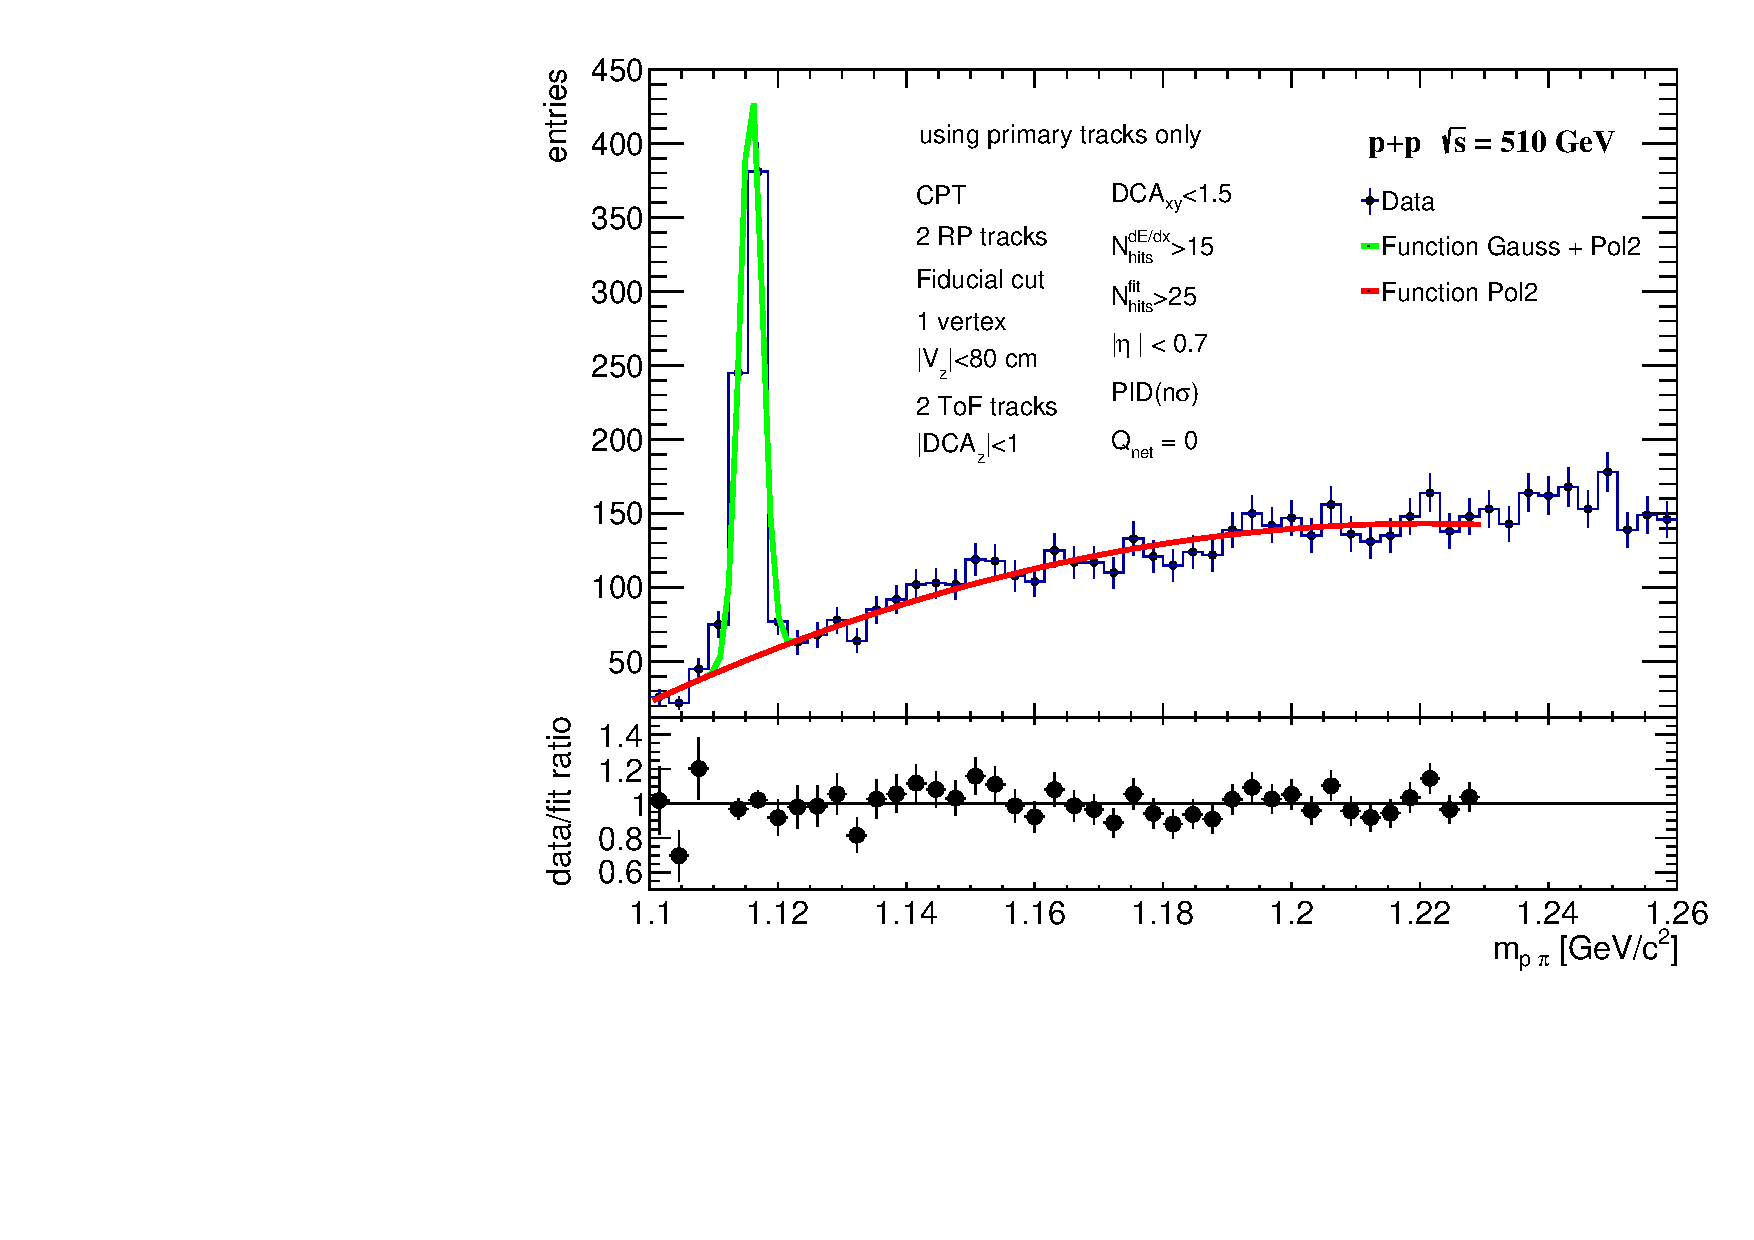
\includegraphics[width=1\textwidth]{figures/LambdaFitQuad.pdf}
    \caption[Distribution of invariant pion proton pairs fitted with Gauss distribution and 2. degree polynomial.]{The distribution of invariant mass of identified $p$ $\pi$ pairs fitted with Gauss distribution function and second degree polynomial.}
    \label{af16}
\end{figure}
\FloatBarrier

%\FloatBarrier
%\begin{table}[ht]
   %    \centering
%        \begin{tabular}{c|c}
%           $p_0$ & $-1.105$ $ \pm$ $ 0.0002$(stat) $10^{4}$\\ \hline
%           $p_1$ & $1.829$ $ \pm$ $ 0.0002$(stat) $10^4$ \\ \hline
%           $p_2$ & $-7.48$ $ \pm$ $ 0.01$(stat) $10^3$ \\ \hline
%           $A$ & $3.6$ $ \pm$ $ 0.2$(stat) $10^3$ \\ \hline
%           $\mu$ & $1.11567$ $\pm$ $ 0.00007$(stat) \\ \hline
%           $\sigma$ & $1.71$ $ \pm$ $ 0.07$(stat) $10^{-3}$ \\ \hline
%           $a$ & $1.1105$ \\ \hline
%           $b$ & $1.1208$ \\ \hline
%           $\chi^2$ & $41$ \\ \hline
%           $ndf$ & $37$  \\ \hline
%           $\frac{\chi^2}{ndf}$ & $1.1$ \\ \hline
%           $y$ & $540 \pm 50$(stat)
%        \end{tabular}
%    \caption[Results for fit 2 of invariant mass of $p \pi$ pairs]{Results of fitted peak for $p$ $\pi^- $ and $\overline{p}$ $\pi^+$ invariant mass distribution, quality of fit and yield. Fitted with Gauss distribution and 2. degree polynomial.}
%    \label{at4}
%\end{table}
%\FloatBarrier

\FloatBarrier
\begin{figure}[ht]
    \centering
    \includegraphics[width=1\textwidth]{figures/hPtMissingLambda.pdf}
    \caption[Distribution of transverse momenta for $p \pi$ pairs]{Distribution of transverse momenta for $p \pi$ pairs.}
    \label{af77}
\end{figure}
\FloatBarrier

\newpage
\chapter*{Summary}
Despite its important role in high-energy physics, the Pomeron remains a mysterious object. In this thesis, the Double \Pom omeron exchange is studied and compared to experimental data from diffractive processes measured at experiment STAR, CMS and ISR.
\newline
Chapter 1 begins with introduction to particle physics and to the area of physics which studies diffractive events on top of establishing certain kinematic variables and categorization of scatterings. This chapter ends with discussing relevant recent results in particle diffraction. Chapter 2 continues with a description of the experiment all the way from establishing what Brookhaven National Laboratory and the Relativistic Heavy Ion Collider are to depicting the different detectors installed at the experiment STAR. Crucial role plays the Roman Pot system which registers forward scattered protons and measures their momentum. That enables the STAR collaboration, as the only physics collaboration to do so, to measure diffractive events and differ between exclusive and inclusive events. Chapter 3 characterizes the data sample used for analysis and explains all the various conditions imposed on analyzed events to select those with the most potential. Part of this chapter is particle identification, which is done based on energy loss from the Time Projection Chamber. 
\newline
Finally, chapter 4 discusses the results from the analyzed proton-proton collisions at $\sqrt{s}=510$ GeV data. The focus was on reconstructing particles $K^0_S$ and $\Lambda^0$, which are created through the Double \Pom omeron Exchange mechanism. The reconstructions were done using the major decay channels: $\pi^+ \pi^-$ for $K^0_S$ and $p \pi^-$ for $\Lambda^0$. Peaks for both particles were significant enough to be fitted with Gauss distribution and polynomials to model background. All fitted values for invariant mass of particles $K^0_S$ and $\Lambda^0$ corresponded with results from PDG. Part of the peak for $\Lambda^0$ was it's antiparticle $\overline{\Lambda^0}$ which decays to $\overline{p} \pi^+$. Distributions of invariant mass for $p \pi^-$ and $\overline{p} \pi^+$ were of similar shape but differently scaled. Invariant mass distribution signal for pairs of $p \pi^-$ was $1.3 \pm 0.1(stat)$ larger than for $\overline{p} \pi^+$ pairs. The exclusivity of measured processes was also discussed. For exclusive production, condition on transverse momentum of $\pi^+ \pi^-$ pairs was imposed. The invariant mass distribution showed structures similar to other measurements in this field. Resonances $f_0$(980) and $f_2$(1270) show the presence of something which could possibly be the lightest scalar glueball, but this area of physics needs further study. All the errors included in \autoref{resultS} are statistical. Systematic errors were not calculated but most probably would cause significantly larger uncertainty in the results. 
\newline
Overall, this thesis provides an establishment of the concept of a \Pom omeron, description of the experiment STAR and the analysis of the Double \Pom omeron Exchange in proton-proton collisions at $\sqrt{s}=510$ GeV. The insights gained from this study may broaden knowledge and help in future studies in the area of diffractive events. Aside from that, the work done on this thesis certainly helped in the development of the author. % Summary


%In particle physics, the Pomeron is a hypothetical exchange particle that is thought to play a role in the strong force interactions between hadrons, such as protons and neutrons. The Pomeron is characterized by its quantum numbers, such as spin and parity, and its exchange is described by a trajectory in the complex angular momentum plane, known as the Pomeron trajectory. The concept of Pomeron exchange was first introduced in the 1960s to explain the high-energy behavior of hadron-hadron scattering, and it continues to be an active area of research today.


%%%%%%%%%%%% SEZNAM POUŽITÝCH ZDROJŮ (LITERATURA) %%%%%%%%%%%%
\clearpage 
%\chapter*{Bibliography}
\bibliography{bibliography}{}
%\bibliographystyle{aip}
\bibliographystyle{IEEEtran}
\addcontentsline{toc}{chapter}{Bibliography} 
    
%\bibliographystyle{abbrv}

%%%%%%%%%%%% PŘÍLOHY PRÁCE %%%%%%%%%%%%
\newpage 

\appendix 
\cleardoublepage\makeatletter\@openrightfalse\makeatother
\newpage
\chapter{Energy loss momentum graphs divided based on the charge of particles}
\label{appendixA}

\FloatBarrier
\begin{figure}[ht]
    \centering
    \includegraphics[width=1\textwidth]{figures/dEdxPlus.pdf}
    \caption[Graph of momentum of positively charged hadrons against energy loss from TPC]{Graph of momentum of positively charged hadrons against energy loss measured in TPC. All scales are logarithmic.}
    \label{af18}
\end{figure}
\FloatBarrier

\FloatBarrier
\begin{figure}[ht]
    \centering
    \includegraphics[width=1\textwidth]{figures/dEdxMinus.pdf}
    \caption[Graph of momentum of negatively charged hadrons against energy loss from TPC]{Graph of momentum of negatively charged hadrons against energy loss measured in TPC. All scales are logarithmic.}
    \label{af32}
\end{figure}
\FloatBarrier

\newpage
\chapter{Correlation plots of n$\sigma$ for different particle pairs}
\label{appendixB}
\FloatBarrier
\begin{figure}[ht]
    \centering
    \includegraphics[width=1\textwidth]{figures/hNSigmaPiKcorr.pdf}
    \caption[Correlation graph of $n\sigma_{\pi}$ and $n\sigma_{K}$ of measured particles]{Correlation graph of $n_{\sigma}$ of pions on the $x$ axis and $n_{\sigma}$ for kaons on the $y$ axis. Black lines represent the conditions for identification and the red box in the middle the overlay.}
    \label{a1}
\end{figure}
\FloatBarrier

\FloatBarrier
\begin{figure}[ht]
    \centering
    \includegraphics[width=1\textwidth]{figures/hNSigmaPiecorr.pdf}
    \caption[Correlation graph of $n\sigma_{\pi}$ and $n\sigma_{e}$ of measured particles]{Correlation graph of $n_{\sigma}$ for pions on the $x$ axis and $n_{\sigma}$ for electrons on the $y$ axis. Black lines represent the conditions for identification and the red box in the middle the overlay.}
    \label{a2}
\end{figure}
\FloatBarrier

\FloatBarrier
\begin{figure}[ht]
    \centering
    \includegraphics[width=1\textwidth]{figures/hNSigmaPecorr.pdf}
    \caption[Correlation graph of $n\sigma_{p}$ and $n\sigma_{e}$ of measured particles]{Correlation graph of $n_{\sigma}$ for protons on the $x$ axis and $n_{\sigma}$ for electrons on the $y$ axis. Black lines represent the conditions for identification and the red box in the middle the overlay.}
    \label{a3}
\end{figure}
\FloatBarrier

\FloatBarrier
\begin{figure}[ht]
    \centering
    \includegraphics[width=1\textwidth]{figures/hNSigmaKecorr.pdf}
    \caption[Correlation graph of $n\sigma_{K}$ and $n\sigma_{e}$ of measured particles]{Correlation graph of $n_{\sigma}$ for kaons on the $x$ axis and $n_{\sigma}$ for electrons on the $y$ axis. Black lines represent the conditions for identification and the red box in the middle the overlay.}
    \label{a4}
\end{figure}
\FloatBarrier

\FloatBarrier
\begin{figure}[ht]
    \centering
    \includegraphics[width=1\textwidth]{figures/hNSigmaKPcorr.pdf}
    \caption[Correlation graph of $n\sigma_{K}$ and $n\sigma_{p}$ of measured particles]{Correlation graph of $n_{\sigma}$ for kaons on the $x$ axis and $n_{\sigma}$ for protons on the $y$ axis. Black lines represent the conditions for identification and the red box in the middle the overlay.}
    \label{a4}
\end{figure}
\FloatBarrier

\FloatBarrier
\begin{figure}[ht]
    \centering
    \includegraphics[width=1\textwidth]{figures/hNSigmaKPicorr.pdf}
    \caption[Correlation graph of $n\sigma_{K}$ and $n\sigma_{\pi}$ of measured particles]{Correlation graph of $n_{\sigma}$ for kaons on the $x$ axis and $n_{\sigma}$ for pions on the $y$ axis. Black lines represent the conditions for identification and the red box in the middle the overlay.}
    \label{a4}
\end{figure}
\FloatBarrier

\FloatBarrier
\begin{figure}[ht]
    \centering
    \includegraphics[width=1\textwidth]{figures/hNSigmaPKcorr.pdf}
    \caption[Correlation graph of $n\sigma_{p}$ and $n\sigma_{K}$ of measured particles]{Correlation graph of $n_{\sigma}$ for protons on the $x$ axis and $n_{\sigma}$ for kaons on the $y$ axis. Black lines represent the conditions for identification and the red box in the middle the overlay.}
    \label{a4}
\end{figure}
\FloatBarrier

\FloatBarrier
\begin{figure}[ht]
    \centering
    \includegraphics[width=1\textwidth]{figures/hNSigmaPPicorr.pdf}
    \caption[Correlation graph of $n\sigma_{p}$ and $n\sigma_{\pi}$ of measured particles]{Correlation graph of $n_{\sigma}$ for protons on the $x$ axis and $n_{\sigma}$ for pions on the $y$ axis. Black lines represent the conditions for identification and the red box in the middle the overlay.}
    \label{a4}
\end{figure}
\FloatBarrier

%\chapter{Variable distributions for two hadrons events}
%\label{rapAndPhi}

\end{document} 